% Generated by build_corner_treatment_figure_report.py -- do not edit by hand; rerun the script.
\documentclass[11pt]{article}
\usepackage[a4paper,margin=0.8in]{geometry}
\usepackage[T1]{fontenc}
\usepackage[utf8]{inputenc}
\usepackage[french]{babel}
\usepackage{amsmath,amssymb}
\usepackage{booktabs}
\usepackage{graphicx}
\usepackage{adjustbox}
\usepackage{float}
\usepackage{xcolor}
\usepackage{pdflscape}
\usepackage{url}
\urlstyle{tt}
\usepackage[colorlinks=true,allcolors=blue!55!black]{hyperref}
\title{Down-and-out put --- traitements du coin sur le domaine complet : figures}
\author{}
\date{2026-09-24}
\begin{document}
\maketitle
\tableofcontents
\clearpage
Recueil des figures et tables produites par les scripts d'agrégation, sans aucun recalcul : chaque légende indique ce qui est tracé ; les chemins des artefacts sources sont donnés en tête de section. Notation : $\Delta=K-B$, $V_{DOD}$ le prix du digital down-and-out, $\xi=\ln(s/B)/(\sigma\sqrt{2(T-t)})$, $\chi$ le cutoff de l'enrichissement, $N_{0.1}=\{|s-B|+(T-t)\le0.1\}$ la fenêtre de coin des métriques.

\section{Comparaison entre configurations (médianes sur les graines)}
Métriques, toutes calculées sur la grille d'évaluation $300\times100$ de $\Omega=(B,s_\infty)\times(0,T)$ (pas $0.008$ en $s$, $0.01$ en $t$), avec $N_w=\{(s,t):|s-B|+(T-t)\le w\}$ la fenêtre de coin, $w=0.1$ :
\[ \mathrm{rel}_{L^2}(A)=\frac{\|\Phi_\theta-V_{DO}\|_{L^2(A)}}{\|V_{DO}\|_{L^2(A)}}, \qquad A\in\{\Omega\setminus N_{0.1}\ (\text{hors coin}),\ \Omega\ (\text{global}),\ N_{0.1}\ (\text{coin})\}, \]\[ \text{best loss}=\min_k\ \frac{1}{n_f}\sum_{(s,t)\in\text{batch}_k}\big(\mathcal L^{BS}\Phi_\theta(s,t)\big)^2, \qquad \text{max\_abs}=\max_{A}|\Phi_\theta-V_{DO}|. \]
Ces normes portent sur la \emph{valeur} $\Phi_\theta-V_{DO}$, champ continu à dérivée bornée : un raffinement de la grille à $2400\times800$ change chaque chiffre de moins de $1{,}3\,\%$ (vérifié sur trois runs, section 15.5 du document de méthodologie). Chaque point est une graine maîtresse, le losange plein la médiane sur les graines. \textbf{Collocation} : les runs de lissage (section 11.1 de la méthodologie) excluent $N_{0.1}$ de la collocation ; les runs de soustraction et d'enrichissement incluent le coin, il n'y a rien à exclure --- l'étiquette de l'axe le rappelle. Source : \path{data/aggregate_terminal_function_comparison/20260923_wholedomain_corner_treatments_iters50000}.
\begin{figure}[H]
\centering

\includegraphics[width=\linewidth]{figures/terminal_function_comparison.png}
\caption{De gauche à droite, de haut en bas : $\mathrm{rel}_{L^2}(\Omega\setminus N_{0.1})$ (métrique de comparaison), $\mathrm{rel}_{L^2}(\Omega)$, $\mathrm{rel}_{L^2}(N_{0.1})$ et la meilleure perte intérieure ; 50000 itérations, $\varepsilon=0.1$ pour les runs de lissage, 5 graines par configuration.}
\label{fig:comparison}
\end{figure}

\begin{table}[H]
\centering
\scriptsize
\begin{adjustbox}{max width=\textwidth}
\begin{tabular}{lccccccc}
\toprule
\textbf{Configuration} & \textbf{n} & \textbf{`rel\_l2\_outside\_corner`} & \textbf{`rel\_l2\_global`} & \textbf{`rel\_l2\_corner`} & \textbf{`max\_abs\_error\_outside\_corner`} & \textbf{`best\_loss`} & \textbf{`best\_iter`} \\
\midrule
Raw payoff $(K-s)^+$ [whole domain: corner in collocation] & 5 & 5.205e-01 [4.942e-01, 6.137e-01] & 5.237e-01 [4.993e-01, 6.130e-01] & 5.782e-01 [5.688e-01, 6.018e-01] & 1.226e-01 [1.201e-01, 1.260e-01] & 1.740e-04 [9.422e-05, 2.376e-04] & 37526 [22919, 49801] \\
Black-Scholes put price (ordinary autograd route) [whole domain: corner in collocation] & 5 & 2.773e-01 [1.515e-01, 4.873e-01] & 3.023e-01 [2.043e-01, 4.934e-01] & 5.858e-01 [5.769e-01, 6.012e-01] & 1.108e-01 [1.022e-01, 2.083e-01] & 1.767e-04 [1.589e-04, 3.675e-04] & 45192 [30027, 48663] \\
Black-Scholes put price (two-term analytic-residual route) [whole domain: corner in collocation] & 5 & 1.419e-01 [1.393e-01, 2.632e-01] & 1.960e-01 [1.952e-01, 2.919e-01] & 5.912e-01 [5.826e-01, 5.919e-01] & 1.085e-01 [1.032e-01, 1.097e-01] & 2.602e-04 [2.410e-04, 3.153e-04] & 47665 [35805, 49823] \\
Split-semigroup profile [whole domain: corner in collocation] & 5 & 2.825e-01 [1.226e-01, 4.399e-01] & 3.067e-01 [1.846e-01, 4.493e-01] & 5.844e-01 [5.758e-01, 5.931e-01] & 1.080e-01 [9.391e-02, 1.710e-01] & 2.108e-04 [9.873e-05, 1.621e-03] & 48573 [45371, 49508] \\
Exact subtraction, raw payoff profile & 5 & 4.549e-01 [4.537e-01, 4.559e-01] & 4.418e-01 [4.407e-01, 4.428e-01] & 5.381e-05 [1.812e-05, 1.093e-04] & 1.176e-01 [1.174e-01, 1.177e-01] & 2.581e-07 [6.530e-08, 3.878e-07] & 47907 [46834, 48332] \\
Exact subtraction, Black-Scholes profile & 5 & 4.687e-03 [2.116e-03, 1.422e-02] & 4.552e-03 [2.055e-03, 1.381e-02] & 4.335e-05 [2.693e-05, 6.171e-05] & 2.224e-03 [7.103e-04, 5.538e-03] & 1.711e-08 [1.044e-08, 2.687e-08] & 49751 [33591, 49974] \\
Exact subtraction, split-semigroup profile & 5 & 3.968e-03 [9.426e-04, 5.193e-03] & 3.854e-03 [9.156e-04, 5.044e-03] & 4.054e-05 [3.062e-05, 4.418e-05] & 1.226e-03 [2.327e-04, 1.928e-03] & 1.057e-08 [8.780e-09, 2.868e-08] & 49470 [48857, 49859] \\
Corner enrichment, raw payoff profile & 5 & 4.557e-01 [4.543e-01, 4.580e-01] & 4.426e-01 [4.412e-01, 4.449e-01] & 6.418e-04 [5.626e-04, 1.501e-03] & 1.177e-01 [1.174e-01, 1.184e-01] & 6.160e-07 [4.150e-07, 2.090e-06] & 45156 [30595, 49049] \\
Corner enrichment, Black-Scholes profile & 5 & 7.316e-03 [2.216e-03, 1.764e-02] & 7.108e-03 [2.160e-03, 1.713e-02] & 7.854e-04 [5.115e-04, 1.058e-03] & 2.979e-03 [3.960e-04, 7.044e-03] & 2.849e-07 [1.490e-07, 5.603e-07] & 49124 [20057, 49920] \\
Corner enrichment, split-semigroup profile & 5 & 6.854e-03 [2.889e-03, 1.473e-02] & 6.658e-03 [2.813e-03, 1.431e-02] & 8.729e-04 [4.331e-04, 1.359e-03] & 2.900e-03 [4.084e-04, 5.850e-03] & 4.405e-07 [1.869e-07, 9.281e-07] & 45456 [26131, 49224] \\
\bottomrule
\end{tabular}
\end{adjustbox}
\caption{$\mathrm{rel}_{L^2}(\Omega\setminus N_{0.1})$, $\mathrm{rel}_{L^2}(\Omega)$, $\mathrm{rel}_{L^2}(N_{0.1})$, $\max_{\Omega\setminus N_{0.1}}|\Phi_\theta-V_{DO}|$, meilleure perte et itération correspondante ; médiane [min, max] sur les graines (\texttt{table.md}).}
\label{tab:metrics}
\end{table}

\section{Diagnostics à partir des modèles sauvegardés}
Mêmes modèles, même grille ; aucun réentraînement. Bandes en $s$ : $\mathcal B=[s_1,s_2]\times(0,T)\setminus N_{0.1}$, $\mathrm{rel}_{L^2}(\mathcal B)=\|\Phi_\theta-V_{DO}\|_{L^2(\mathcal B)}/\|V_{DO}\|_{L^2(\mathcal B)}$ et $\mathrm{abs}_{L^2}(\mathcal B)=\|\Phi_\theta-V_{DO}\|_{L^2(\mathcal B)}$ avec $\|f\|_{L^2(\mathcal B)}=(\sum_{\mathcal B}f^2\,\Delta s\,\Delta t)^{1/2}$. La bande $[2,s_\infty]$ est à lire en absolu : $\|V_{DO}\|_{L^2}$ y vaut $1.1\times10^{-4}$, une erreur relative de $3$ y correspond à une erreur absolue de $3\times10^{-4}$.
\begin{figure}[H]
\centering

\includegraphics[width=\linewidth]{figures/rel_l2_vs_excluded_area_by_window_shape.png}
\caption{$\mathrm{rel}_{L^2}(\Omega\setminus N)$ pour trois familles de fenêtre $N$ autour du coin (losange $N_w=\{|s-B|+\tau\le w\}$, parabole $N_c=\{|s-B|\le cB\sigma\sqrt\tau\}$, hyperbole $N_d=\{\tau(s-B)\le d\}$, $\tau=T-t$), en fonction de la fraction d'aire exclue $|N\cap\Omega|/|\Omega|$ ; un panneau par configuration.}
\label{fig:window-shapes}
\end{figure}

\begin{figure}[H]
\centering

\includegraphics[width=\linewidth]{figures/band_network_contribution.png}
\caption{Bande $\mathcal B=\{0.1<|s-B|<0.3\}$ (tout $t$) : $\|\Phi_\theta-V_{DO}\|_{L^2(\mathcal B)}$ (losanges, solution entraînée) contre $\|g_2-V_{DO}\|_{L^2(\mathcal B)}$ (tirets rouges, extension seule, sans réseau) et $\|V_{DO}\|_{L^2(\mathcal B)}$ (pointillés, échelle). Un rapport proche de 1 signifie que le réseau n'apporte rien dans la bande.}
\label{fig:band}
\end{figure}

\begin{table}[H]
\centering
\scriptsize
\begin{adjustbox}{max width=\textwidth}
\begin{tabular}{lcccc}
\toprule
\textbf{Configuration} & \textbf{[0.6, 0.7]} & \textbf{[0.7, 1]} & \textbf{[1, 2]} & \textbf{[2, 3]} \\
\midrule
Raw payoff $(K-s)^+$ [whole domain: corner in collocation] & 2.285e-01 [2.131e-01, 2.535e-01] & 3.925e-01 [3.727e-01, 4.010e-01] & 1.334e+00 [1.301e+00, 1.391e+00] & 1.197e+02 [2.239e+01, 2.211e+02] \\
Black-Scholes put price (ordinary autograd route) [whole domain: corner in collocation] & 2.210e-01 [2.181e-01, 2.260e-01] & 9.116e-02 [7.458e-02, 1.110e-01] & 9.847e-02 [9.027e-02, 1.151e-01] & 1.638e+02 [6.351e+01, 3.214e+02] \\
Black-Scholes put price (two-term analytic-residual route) [whole domain: corner in collocation] & 2.223e-01 [2.034e-01, 2.368e-01] & 8.772e-02 [7.692e-02, 1.050e-01] & 6.234e-02 [4.616e-02, 1.557e-01] & 5.325e+01 [2.418e+01, 1.621e+02] \\
Split-semigroup profile [whole domain: corner in collocation] & 2.209e-01 [1.831e-01, 2.236e-01] & 8.696e-02 [6.761e-02, 9.072e-02] & 8.656e-02 [4.545e-02, 1.103e-01] & 1.742e+02 [2.743e+01, 2.862e+02] \\
Exact subtraction, raw payoff profile & 3.962e-02 [3.929e-02, 4.073e-02] & 3.397e-01 [3.389e-01, 3.409e-01] & 1.294e+00 [1.291e+00, 1.294e+00] & 6.964e+00 [2.612e+00, 9.760e+00] \\
Exact subtraction, Black-Scholes profile & 1.406e-04 [4.359e-05, 1.708e-04] & 1.831e-04 [4.396e-05, 2.910e-04] & 1.115e-03 [6.156e-04, 1.806e-03] & 3.162e+00 [1.429e+00, 9.626e+00] \\
Exact subtraction, split-semigroup profile & 1.002e-04 [8.625e-05, 3.701e-04] & 1.190e-04 [8.630e-05, 4.891e-04] & 5.204e-04 [3.707e-04, 1.733e-03] & 2.686e+00 [4.651e-01, 3.513e+00] \\
Corner enrichment, raw payoff profile & 3.947e-02 [3.912e-02, 4.072e-02] & 3.404e-01 [3.391e-01, 3.427e-01] & 1.296e+00 [1.292e+00, 1.300e+00] & 2.429e+00 [1.426e+00, 8.814e+00] \\
Corner enrichment, Black-Scholes profile & 4.394e-04 [2.012e-04, 1.088e-03] & 5.836e-04 [2.333e-04, 1.345e-03] & 1.652e-03 [1.563e-03, 2.709e-03] & 4.945e+00 [1.372e+00, 1.193e+01] \\
Corner enrichment, split-semigroup profile & 5.251e-04 [2.606e-04, 1.195e-03] & 8.443e-04 [2.944e-04, 1.164e-03] & 2.998e-03 [1.120e-03, 8.337e-03] & 4.636e+00 [1.044e+00, 9.939e+00] \\
\bottomrule
\end{tabular}
\end{adjustbox}
\caption{$\mathrm{rel}_{L^2}(\mathcal B)$ par bande $\mathcal B$ de $s$ (tout $t$, $N_{0.1}$ retirée), médiane [min, max] sur les graines.}
\label{tab:bands-rel}
\end{table}

\begin{table}[H]
\centering
\scriptsize
\begin{adjustbox}{max width=\textwidth}
\begin{tabular}{lcccc}
\toprule
\textbf{Configuration} & \textbf{[0.6, 0.7]} & \textbf{[0.7, 1]} & \textbf{[1, 2]} & \textbf{[2, 3]} \\
\midrule
Raw payoff $(K-s)^+$ [whole domain: corner in collocation] & 6.880e-03 [6.418e-03, 7.635e-03] & 2.615e-02 [2.483e-02, 2.671e-02] & 2.680e-02 [2.614e-02, 2.794e-02] & 1.339e-02 [2.506e-03, 2.474e-02] \\
Black-Scholes put price (ordinary autograd route) [whole domain: corner in collocation] & 6.655e-03 [6.567e-03, 6.806e-03] & 6.073e-03 [4.968e-03, 7.398e-03] & 1.978e-03 [1.813e-03, 2.312e-03] & 1.833e-02 [7.106e-03, 3.596e-02] \\
Black-Scholes put price (two-term analytic-residual route) [whole domain: corner in collocation] & 6.695e-03 [6.125e-03, 7.131e-03] & 5.844e-03 [5.124e-03, 6.997e-03] & 1.252e-03 [9.273e-04, 3.128e-03] & 5.958e-03 [2.706e-03, 1.813e-02] \\
Split-semigroup profile [whole domain: corner in collocation] & 6.652e-03 [5.514e-03, 6.733e-03] & 5.793e-03 [4.504e-03, 6.043e-03] & 1.739e-03 [9.131e-04, 2.215e-03] & 1.950e-02 [3.069e-03, 3.203e-02] \\
Exact subtraction, raw payoff profile & 1.193e-03 [1.183e-03, 1.227e-03] & 2.263e-02 [2.258e-02, 2.271e-02] & 2.599e-02 [2.593e-02, 2.601e-02] & 7.793e-04 [2.923e-04, 1.092e-03] \\
Exact subtraction, Black-Scholes profile & 4.234e-06 [1.313e-06, 5.143e-06] & 1.219e-05 [2.929e-06, 1.938e-05] & 2.240e-05 [1.237e-05, 3.629e-05] & 3.539e-04 [1.599e-04, 1.077e-03] \\
Exact subtraction, split-semigroup profile & 3.019e-06 [2.597e-06, 1.115e-05] & 7.929e-06 [5.749e-06, 3.258e-05] & 1.045e-05 [7.447e-06, 3.482e-05] & 3.006e-04 [5.205e-05, 3.931e-04] \\
Corner enrichment, raw payoff profile & 1.189e-03 [1.178e-03, 1.226e-03] & 2.268e-02 [2.259e-02, 2.283e-02] & 2.604e-02 [2.596e-02, 2.612e-02] & 2.718e-04 [1.596e-04, 9.863e-04] \\
Corner enrichment, Black-Scholes profile & 1.323e-05 [6.058e-06, 3.275e-05] & 3.888e-05 [1.554e-05, 8.960e-05] & 3.319e-05 [3.140e-05, 5.443e-05] & 5.533e-04 [1.535e-04, 1.335e-03] \\
Corner enrichment, split-semigroup profile & 1.581e-05 [7.846e-06, 3.597e-05] & 5.624e-05 [1.961e-05, 7.755e-05] & 6.022e-05 [2.249e-05, 1.675e-04] & 5.187e-04 [1.168e-04, 1.112e-03] \\
\bottomrule
\end{tabular}
\end{adjustbox}
\caption{$\mathrm{abs}_{L^2}(\mathcal B)=\|\Phi_\theta-V_{DO}\|_{L^2(\mathcal B)}$ par bande de $s$ (norme discrète pondérée par l'aire des cellules), médiane [min, max] sur les graines.}
\label{tab:bands-abs}
\end{table}

\section{Grecques au strike}
Erreur relative \emph{ponctuelle} en $s=K$, à cinq dates $t\in\{0,0.25,0.5,0.75,0.9\}$ :\[ \mathrm{err}_{\mathrm{rel}}\,\Delta(t)=\frac{|\partial_s\Phi_\theta(K,t)-\partial_sV_{DO}(K,t)|}{|\partial_sV_{DO}(K,t)|},\qquad \mathrm{err}_{\mathrm{rel}}\,\Gamma(t)=\frac{|\partial_{ss}\Phi_\theta(K,t)-\partial_{ss}V_{DO}(K,t)|}{|\partial_{ss}V_{DO}(K,t)|}. \]Côté entraîné : $\partial_s$, $\partial_{ss}$ de $g_1u_\theta$ par deux passes autograd imbriquées au point $(K,t)$, dérivées de $g_2$ en forme fermée (split, soustraction, enrichissement) ou par autograd (lissage Black--Scholes) ; côté référence : dérivée symbolique (sympy, évaluation mpmath) de la forme fermée de Reiner--Rubinstein. Aucune grille n'intervient : ce sont des valeurs ponctuelles, pas des quadratures, donc la largeur du pic de $\partial_{ss}$ au strike n'est pas un problème de résolution. La fragilité est celle d'un point : $\partial_{ss}V_{DO}(K,t)$ change de signe vers $t\approx0.27$, et l'erreur relative est mal conditionnée près de ce zéro (lignes $t=0.25$). Médiane [min, max] sur 5 graines. Source : \path{data/evaluate_greeks_no_corner/20260923_wholedomain_corner_treatments_iters50000}.
\begin{figure}[H]
\centering

\includegraphics[width=\linewidth]{figures/greeks_no_corner.png}
\caption{$\mathrm{err}_{\mathrm{rel}}\,\Gamma(t)$ en fonction de $\tau=T-t$ (log-log), une courbe par configuration (médiane sur les graines ; points pâles : graines). Les tirets verticaux marquent les $\tau$ où $|\partial_{ss}V_{DO}(K,t)|$ est inférieur à $10\,\%$ de son maximum (erreur relative mal conditionnée).}
\label{fig:greeks}
\end{figure}

\begin{table}[H]
\centering
\scriptsize
\begin{adjustbox}{max width=\textwidth}
\begin{tabular}{lccccc}
\toprule
\textbf{Configuration} & \textbf{$t=0$} & \textbf{$t=0.25$} & \textbf{$t=0.5$} & \textbf{$t=0.75$} & \textbf{$t=0.9$} \\
\midrule
Raw payoff $(K-s)^+$ [whole domain: corner in collocation] & 3.404e+00 [3.395e+00, 3.457e+00] & 2.144e+00 [2.110e+00, 2.183e+00] & 1.431e+00 [1.403e+00, 1.476e+00] & 1.124e+00 [1.123e+00, 1.139e+00] & 1.099e+00 [1.093e+00, 1.108e+00] \\
Black-Scholes put price (ordinary autograd route) [whole domain: corner in collocation] & 1.061e-01 [8.447e-02, 2.104e-01] & 1.174e-01 [7.294e-02, 1.301e-01] & 7.653e-02 [6.540e-02, 1.163e-01] & 2.310e-02 [1.987e-02, 6.254e-02] & 6.365e-03 [1.183e-03, 1.017e-02] \\
Black-Scholes put price (two-term analytic-residual route) [whole domain: corner in collocation] & 1.136e-01 [9.276e-02, 3.432e-01] & 9.962e-02 [4.529e-02, 1.573e-01] & 9.880e-02 [6.668e-02, 1.217e-01] & 4.057e-02 [3.292e-02, 6.552e-02] & 1.005e-02 [3.173e-03, 1.794e-02] \\
Split-semigroup profile [whole domain: corner in collocation] & 1.403e-01 [2.910e-02, 1.670e-01] & 1.043e-01 [7.346e-02, 1.312e-01] & 9.082e-02 [3.604e-02, 1.326e-01] & 3.355e-02 [1.747e-02, 6.744e-02] & 1.203e-02 [4.824e-03, 1.908e-02] \\
Exact subtraction, raw payoff profile & 3.228e+00 [3.225e+00, 3.240e+00] & 2.088e+00 [2.085e+00, 2.095e+00] & 1.416e+00 [1.413e+00, 1.418e+00] & 1.103e+00 [1.101e+00, 1.105e+00] & 1.052e+00 [1.050e+00, 1.053e+00] \\
Exact subtraction, Black-Scholes profile & 1.549e-04 [8.349e-05, 6.463e-04] & 1.472e-04 [1.853e-06, 6.461e-04] & 2.426e-04 [5.164e-06, 3.615e-04] & 7.842e-05 [2.869e-05, 3.811e-04] & 7.921e-05 [2.017e-05, 1.380e-04] \\
Exact subtraction, split-semigroup profile & 3.002e-04 [1.269e-04, 7.926e-04] & 1.656e-04 [3.019e-05, 4.315e-04] & 2.074e-04 [1.060e-04, 5.968e-04] & 1.640e-04 [4.401e-05, 3.802e-04] & 1.923e-04 [9.877e-05, 5.444e-04] \\
Corner enrichment, raw payoff profile & 3.232e+00 [3.215e+00, 3.246e+00] & 2.092e+00 [2.080e+00, 2.101e+00] & 1.418e+00 [1.411e+00, 1.420e+00] & 1.105e+00 [1.104e+00, 1.106e+00] & 1.052e+00 [1.041e+00, 1.054e+00] \\
Corner enrichment, Black-Scholes profile & 1.388e-03 [6.775e-04, 1.661e-03] & 7.944e-04 [1.927e-05, 1.635e-03] & 1.193e-03 [5.798e-05, 1.880e-03] & 7.177e-04 [2.937e-04, 1.987e-03] & 6.028e-04 [3.209e-05, 7.496e-04] \\
Corner enrichment, split-semigroup profile & 3.539e-03 [1.628e-03, 6.720e-03] & 8.760e-04 [9.496e-05, 3.735e-03] & 8.006e-04 [2.709e-04, 2.185e-03] & 6.953e-04 [2.344e-04, 2.595e-03] & 1.589e-03 [1.576e-04, 1.871e-03] \\
\bottomrule
\end{tabular}
\end{adjustbox}
\caption{$\mathrm{err}_{\mathrm{rel}}\,\Delta(t)$ au strike, une ligne par configuration, une colonne par $t$ ; médiane [min, max] sur 5 graines.}
\label{tab:greeks-delta}
\end{table}

\begin{table}[H]
\centering
\scriptsize
\begin{adjustbox}{max width=\textwidth}
\begin{tabular}{lccccc}
\toprule
\textbf{Configuration} & \textbf{$t=0$} & \textbf{$t=0.25$} & \textbf{$t=0.5$} & \textbf{$t=0.75$} & \textbf{$t=0.9$} \\
\midrule
Raw payoff $(K-s)^+$ [whole domain: corner in collocation] & 3.839e+00 [3.469e+00, 4.387e+00] & 4.996e+01 [4.764e+01, 5.388e+01] & 2.648e+00 [2.450e+00, 2.704e+00] & 1.191e+00 [1.161e+00, 1.226e+00] & 1.014e+00 [1.007e+00, 1.038e+00] \\
Black-Scholes put price (ordinary autograd route) [whole domain: corner in collocation] & 7.572e-02 [2.776e-03, 1.162e+00] & 4.528e+00 [9.308e-01, 6.155e+00] & 2.925e-01 [1.239e-01, 3.328e-01] & 1.048e-01 [5.227e-02, 1.325e-01] & 6.512e-03 [9.841e-04, 1.276e-02] \\
Black-Scholes put price (two-term analytic-residual route) [whole domain: corner in collocation] & 3.288e-01 [1.566e-02, 7.573e-01] & 2.948e+00 [2.658e-01, 8.400e+00] & 2.913e-01 [3.741e-02, 3.664e-01] & 1.029e-01 [3.643e-03, 1.682e-01] & 1.694e-02 [6.333e-03, 4.024e-02] \\
Split-semigroup profile [whole domain: corner in collocation] & 5.156e-01 [1.257e-01, 1.237e+00] & 2.483e+00 [2.875e-01, 1.475e+01] & 2.460e-01 [1.209e-02, 3.900e-01] & 1.223e-01 [7.815e-02, 2.112e-01] & 1.438e-02 [6.411e-03, 4.540e-02] \\
Exact subtraction, raw payoff profile & 4.017e+00 [3.574e+00, 4.073e+00] & 4.681e+01 [4.250e+01, 4.806e+01] & 2.411e+00 [2.150e+00, 2.451e+00] & 1.083e+00 [9.903e-01, 1.099e+00] & 1.008e+00 [9.435e-01, 1.019e+00] \\
Exact subtraction, Black-Scholes profile & 1.490e-03 [2.459e-04, 6.698e-03] & 6.462e-03 [6.078e-03, 2.409e-02] & 1.076e-03 [5.006e-04, 1.351e-03] & 3.171e-04 [3.742e-05, 4.418e-04] & 8.269e-05 [1.223e-05, 2.208e-04] \\
Exact subtraction, split-semigroup profile & 2.990e-03 [9.200e-04, 1.035e-02] & 5.542e-03 [2.196e-03, 5.806e-02] & 9.687e-04 [3.884e-04, 2.451e-03] & 5.615e-04 [3.282e-04, 9.357e-04] & 5.914e-04 [1.495e-04, 1.274e-03] \\
Corner enrichment, raw payoff profile & 3.929e+00 [3.583e+00, 4.319e+00] & 4.672e+01 [4.584e+01, 4.743e+01] & 2.396e+00 [2.259e+00, 2.438e+00] & 1.060e+00 [1.032e+00, 1.081e+00] & 9.978e-01 [9.804e-01, 1.018e+00] \\
Corner enrichment, Black-Scholes profile & 4.714e-02 [7.676e-03, 1.132e-01] & 6.375e-02 [1.802e-02, 2.470e-01] & 4.873e-03 [2.039e-04, 1.618e-02] & 2.198e-03 [2.634e-04, 4.902e-03] & 9.626e-04 [7.398e-04, 1.694e-03] \\
Corner enrichment, split-semigroup profile & 4.405e-02 [1.123e-03, 7.510e-02] & 1.740e-01 [4.253e-02, 3.060e-01] & 6.199e-03 [4.043e-04, 2.404e-02] & 3.079e-03 [6.961e-04, 4.406e-03] & 4.114e-03 [2.167e-03, 5.759e-03] \\
\bottomrule
\end{tabular}
\end{adjustbox}
\caption{$\mathrm{err}_{\mathrm{rel}}\,\Gamma(t)$ au strike, idem. La colonne $t=0.25$ est mal conditionnée ($\partial_{ss}V_{DO}(K,0.25)=-3.3\times10^{-2}$, proche de son zéro) et n'est pas à lire comme une performance.}
\label{tab:greeks-gamma}
\end{table}

\section{Profils en $s$ et grecques en fonction de $t$ (graine 0)}
Une seule graine, pas de médiane : ces figures montrent \emph{où} l'erreur de chaque traitement se trouve, ce que les métriques intégrées ne disent pas. Évaluation ponctuelle en float64 ; dérivées comme à la section précédente (autograd imbriqué sur $g_1u_\theta$, forme fermée pour $g_2$). Une sous-section par fonction terminale : à fonction terminale fixée, les trois courbes d'un panneau ne diffèrent que par le traitement du coin. Code couleur commun à toutes ces figures : \textbf{orange} lissage (couche de coin, $\varepsilon=0.1$), \textbf{vert} soustraction exacte (Méthode 1), \textbf{violet} enrichissement de coin (Méthode 2) ; \textbf{tirets noirs} forme fermée.
\subsection{Fonction terminale : payoff brut $(K-s)^+$}
Source : \path{data/compare_corner_treatments_profiles/20260924_wholedomain_raw}.
\begin{landscape}
\begin{figure}[H]
\centering
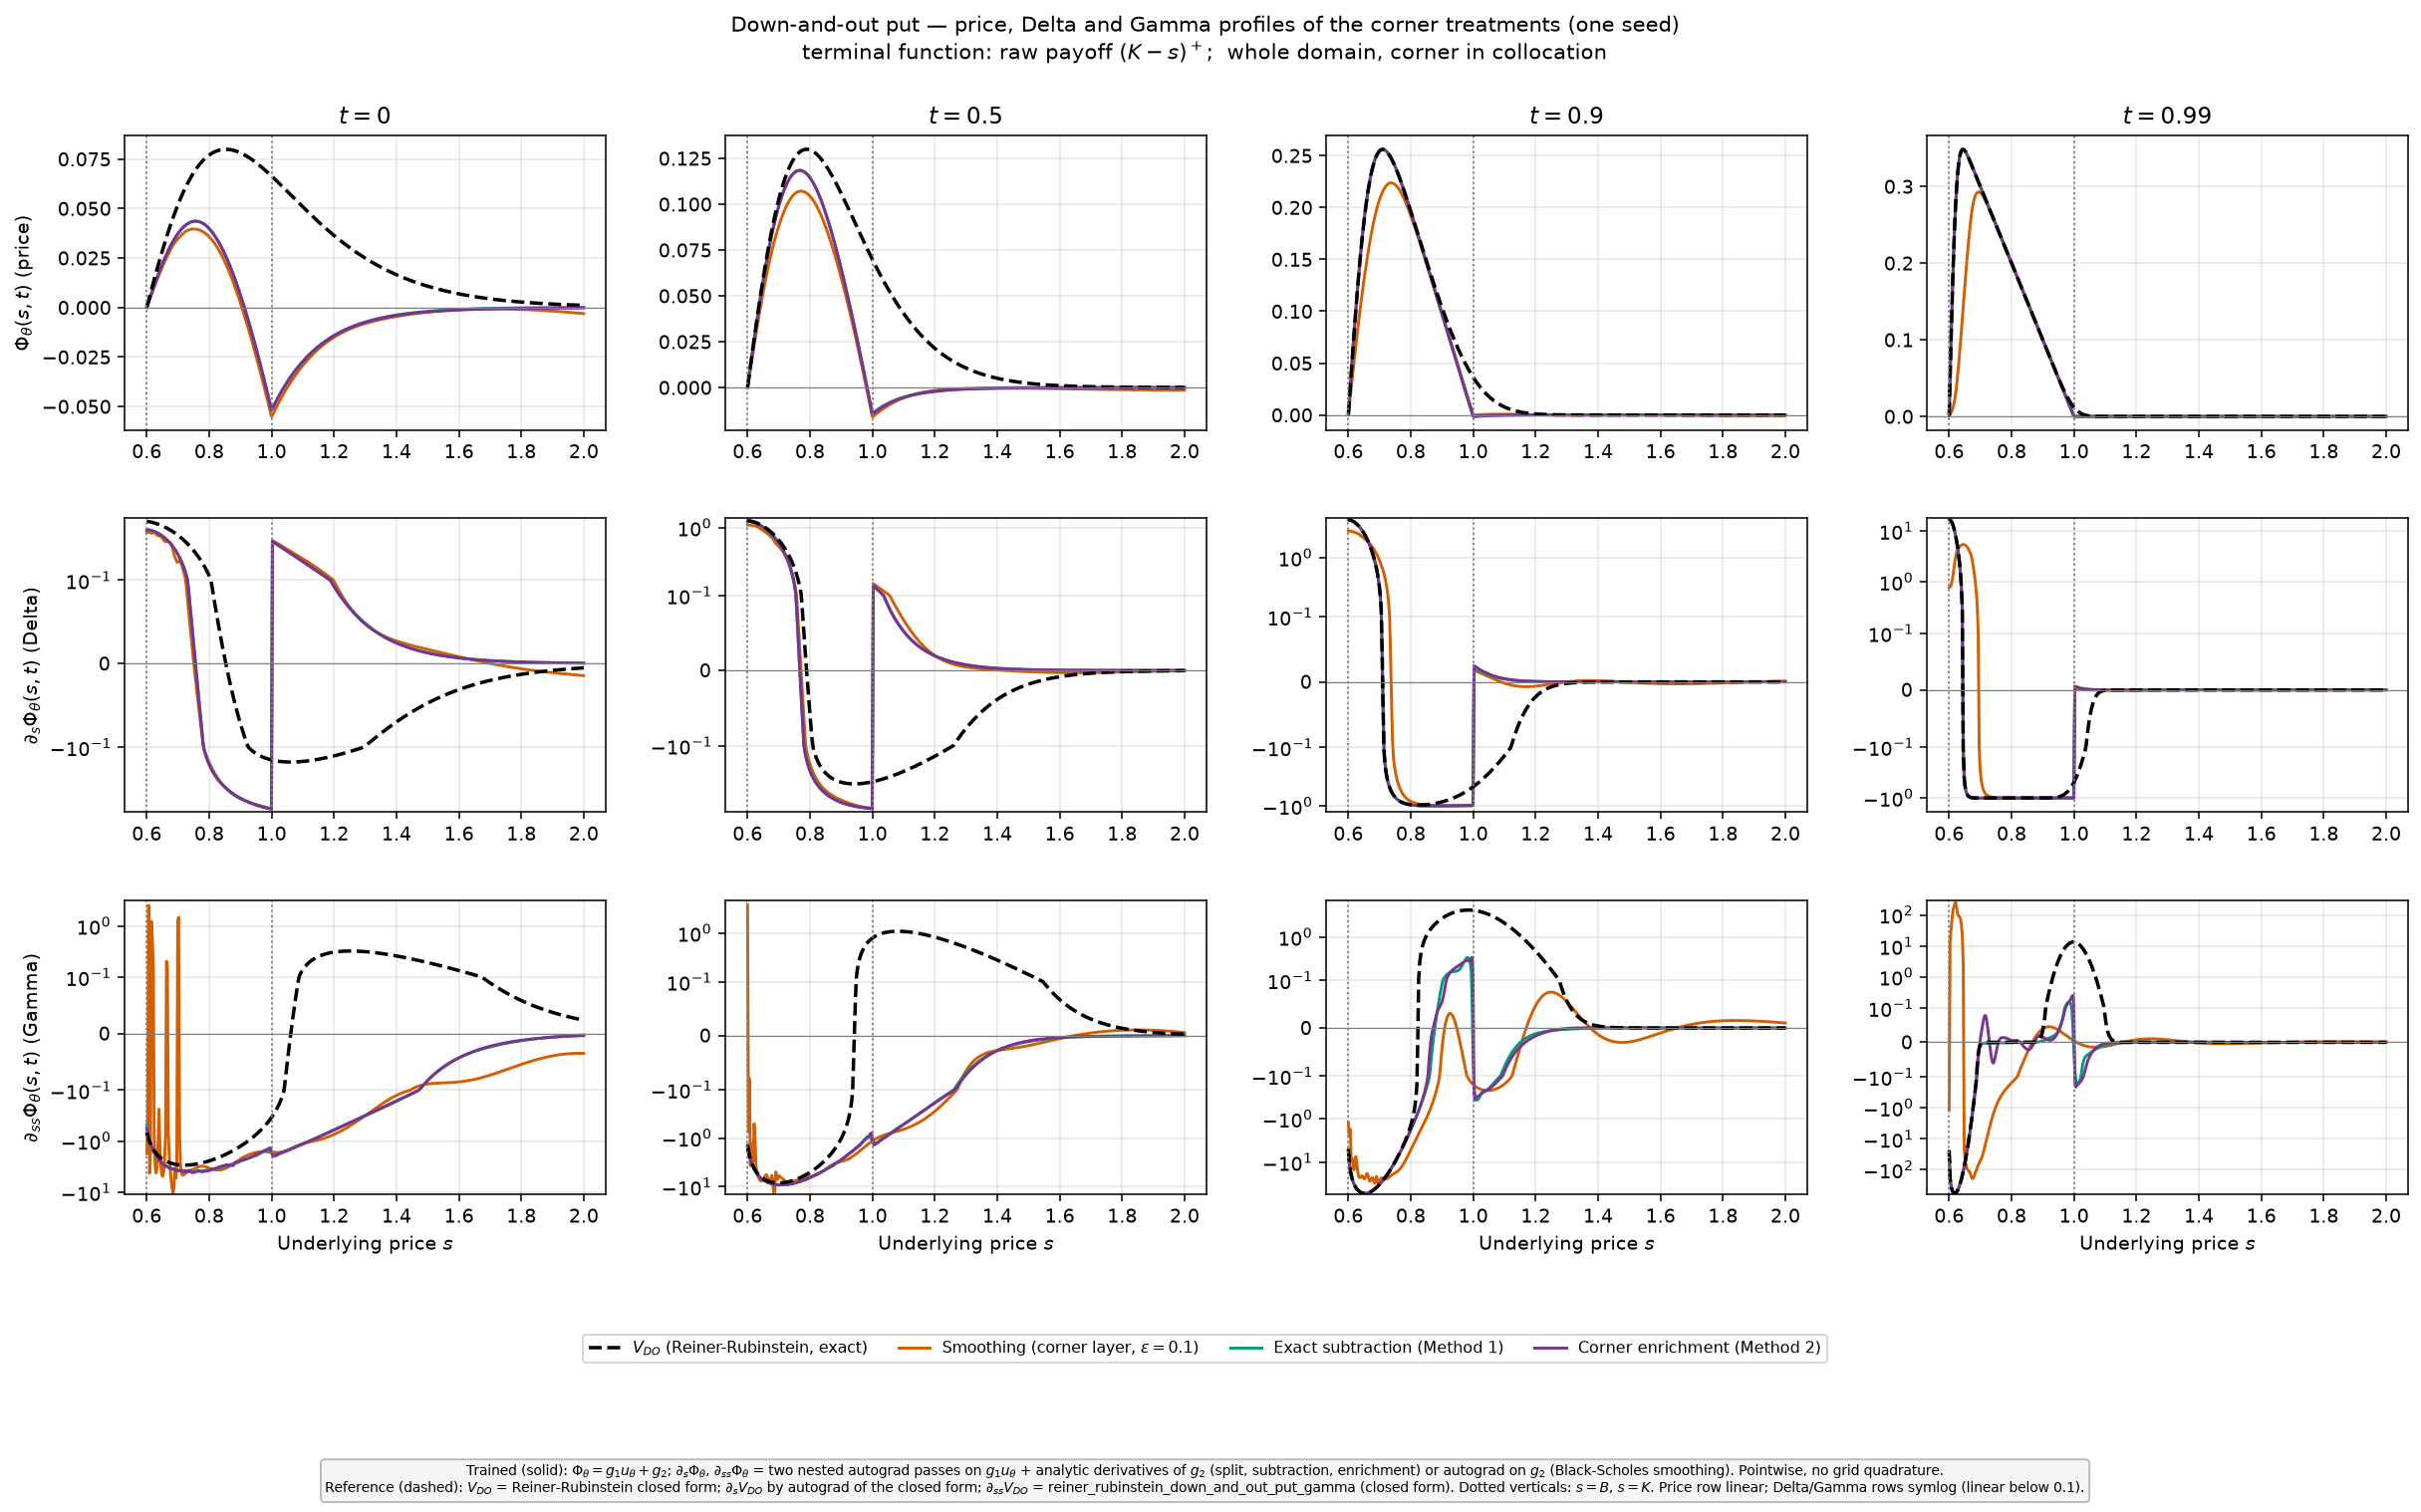
\includegraphics[width=\linewidth,height=0.8\textheight,keepaspectratio]{figures/profiles_price_delta_gamma_raw.png}
\caption{Lignes : $\Phi_\theta(s,t)$, $\partial_s\Phi_\theta(s,t)$, $\partial_{ss}\Phi_\theta(s,t)$ ; colonnes : $t\in\{0,0.5,0.9,0.99\}$ ; forme fermée en tirets noirs. Prix en échelle linéaire ; $\Delta$ et $\Gamma$ en échelle symlog (linéaire sous $0.1$, logarithmique au-delà, des deux côtés de zéro).}
\label{fig:profiles_raw}
\end{figure}

\end{landscape}

\begin{landscape}
\begin{figure}[H]
\centering
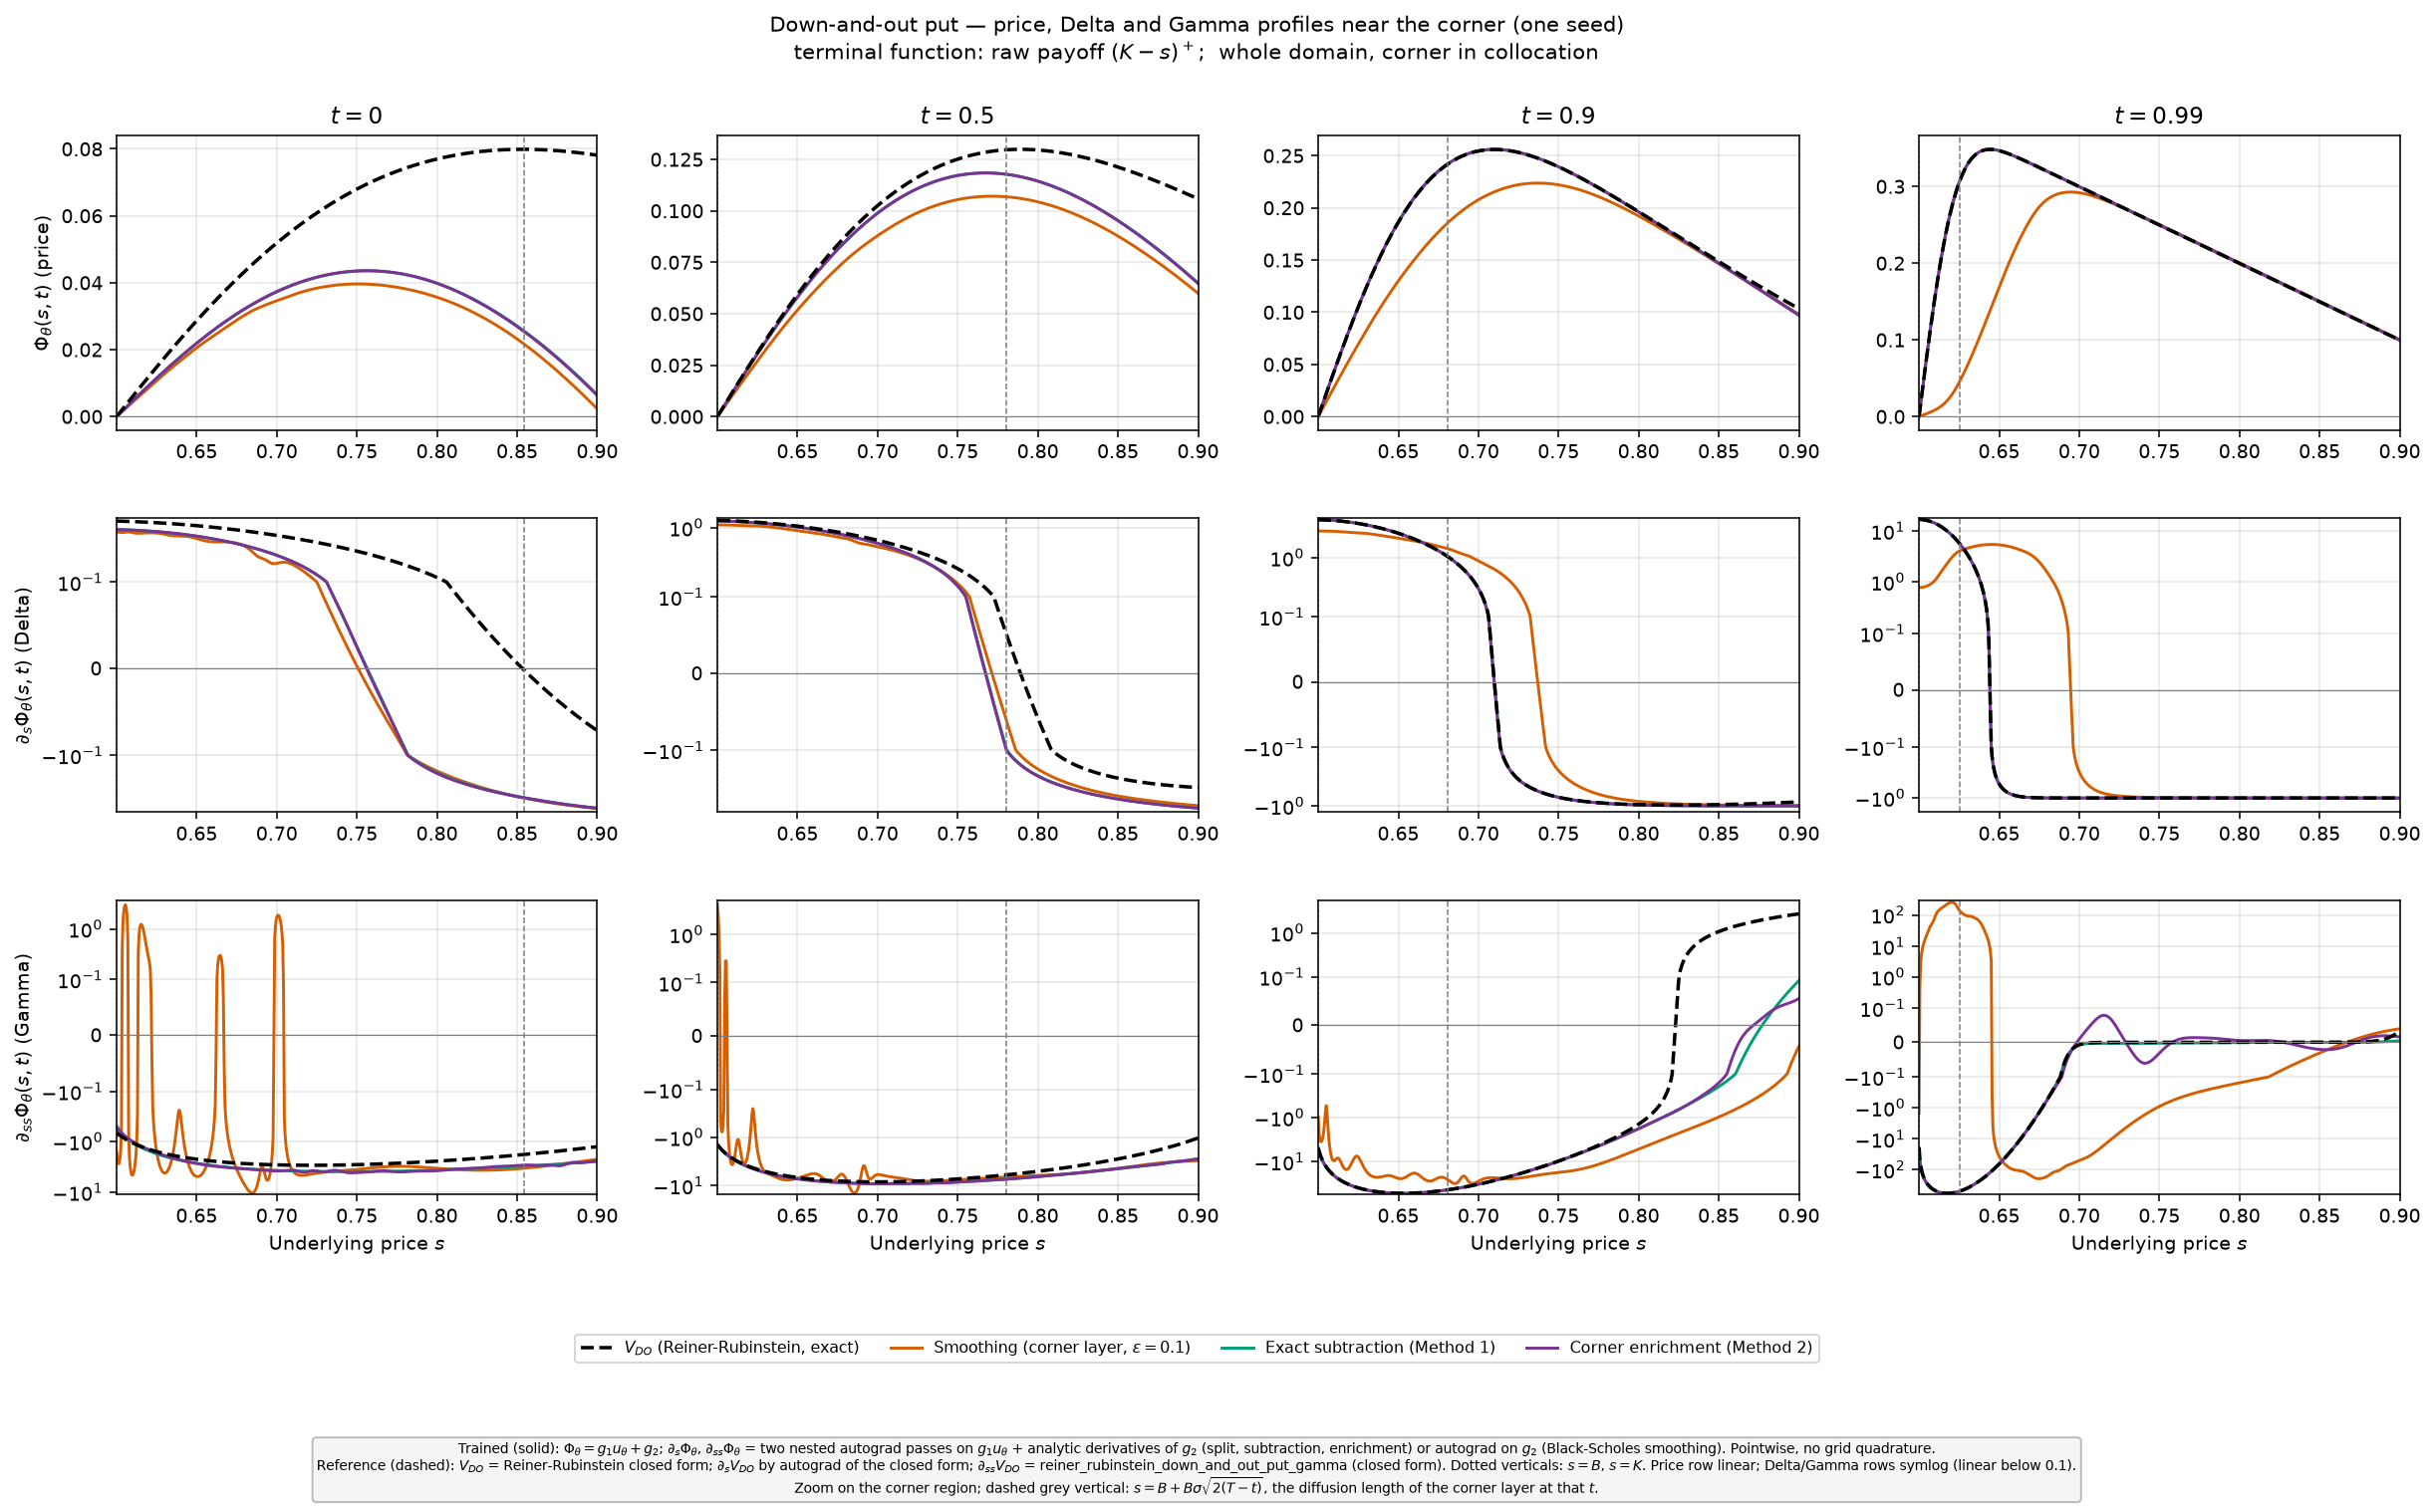
\includegraphics[width=\linewidth,height=0.8\textheight,keepaspectratio]{figures/profiles_price_delta_gamma_corner_zoom_raw.png}
\caption{Même figure, restreinte à la région du coin $s\in(B, B+0.3)$ et évaluée sur sa propre grille dense (600 points, pas $5\times10^{-4}$). Tirets gris verticaux : $s=B+B\sigma\sqrt{2(T-t)}$, la longueur de diffusion de la couche de coin à ce $t$. Les ondulations de $\partial_{ss}\Phi_\theta$ du run de lissage (orange) sont confinées à la bande de transition du cutoff $\zeta((s-B)/\varepsilon)$, $s\in[0.6,0.7]$ : c'est la courbure de $\zeta$ ($\zeta''\sim\varepsilon^{-2}$) que le réseau n'annule pas. La soustraction (vert) est confondue avec la forme fermée sur les trois lignes ; l'enrichissement (violet) l'est aussi hors de la bande de transition de $\chi$, $[0.7,0.9]$.}
\label{fig:profiles-zoom_raw}
\end{figure}

\end{landscape}

\begin{landscape}
\begin{figure}[H]
\centering
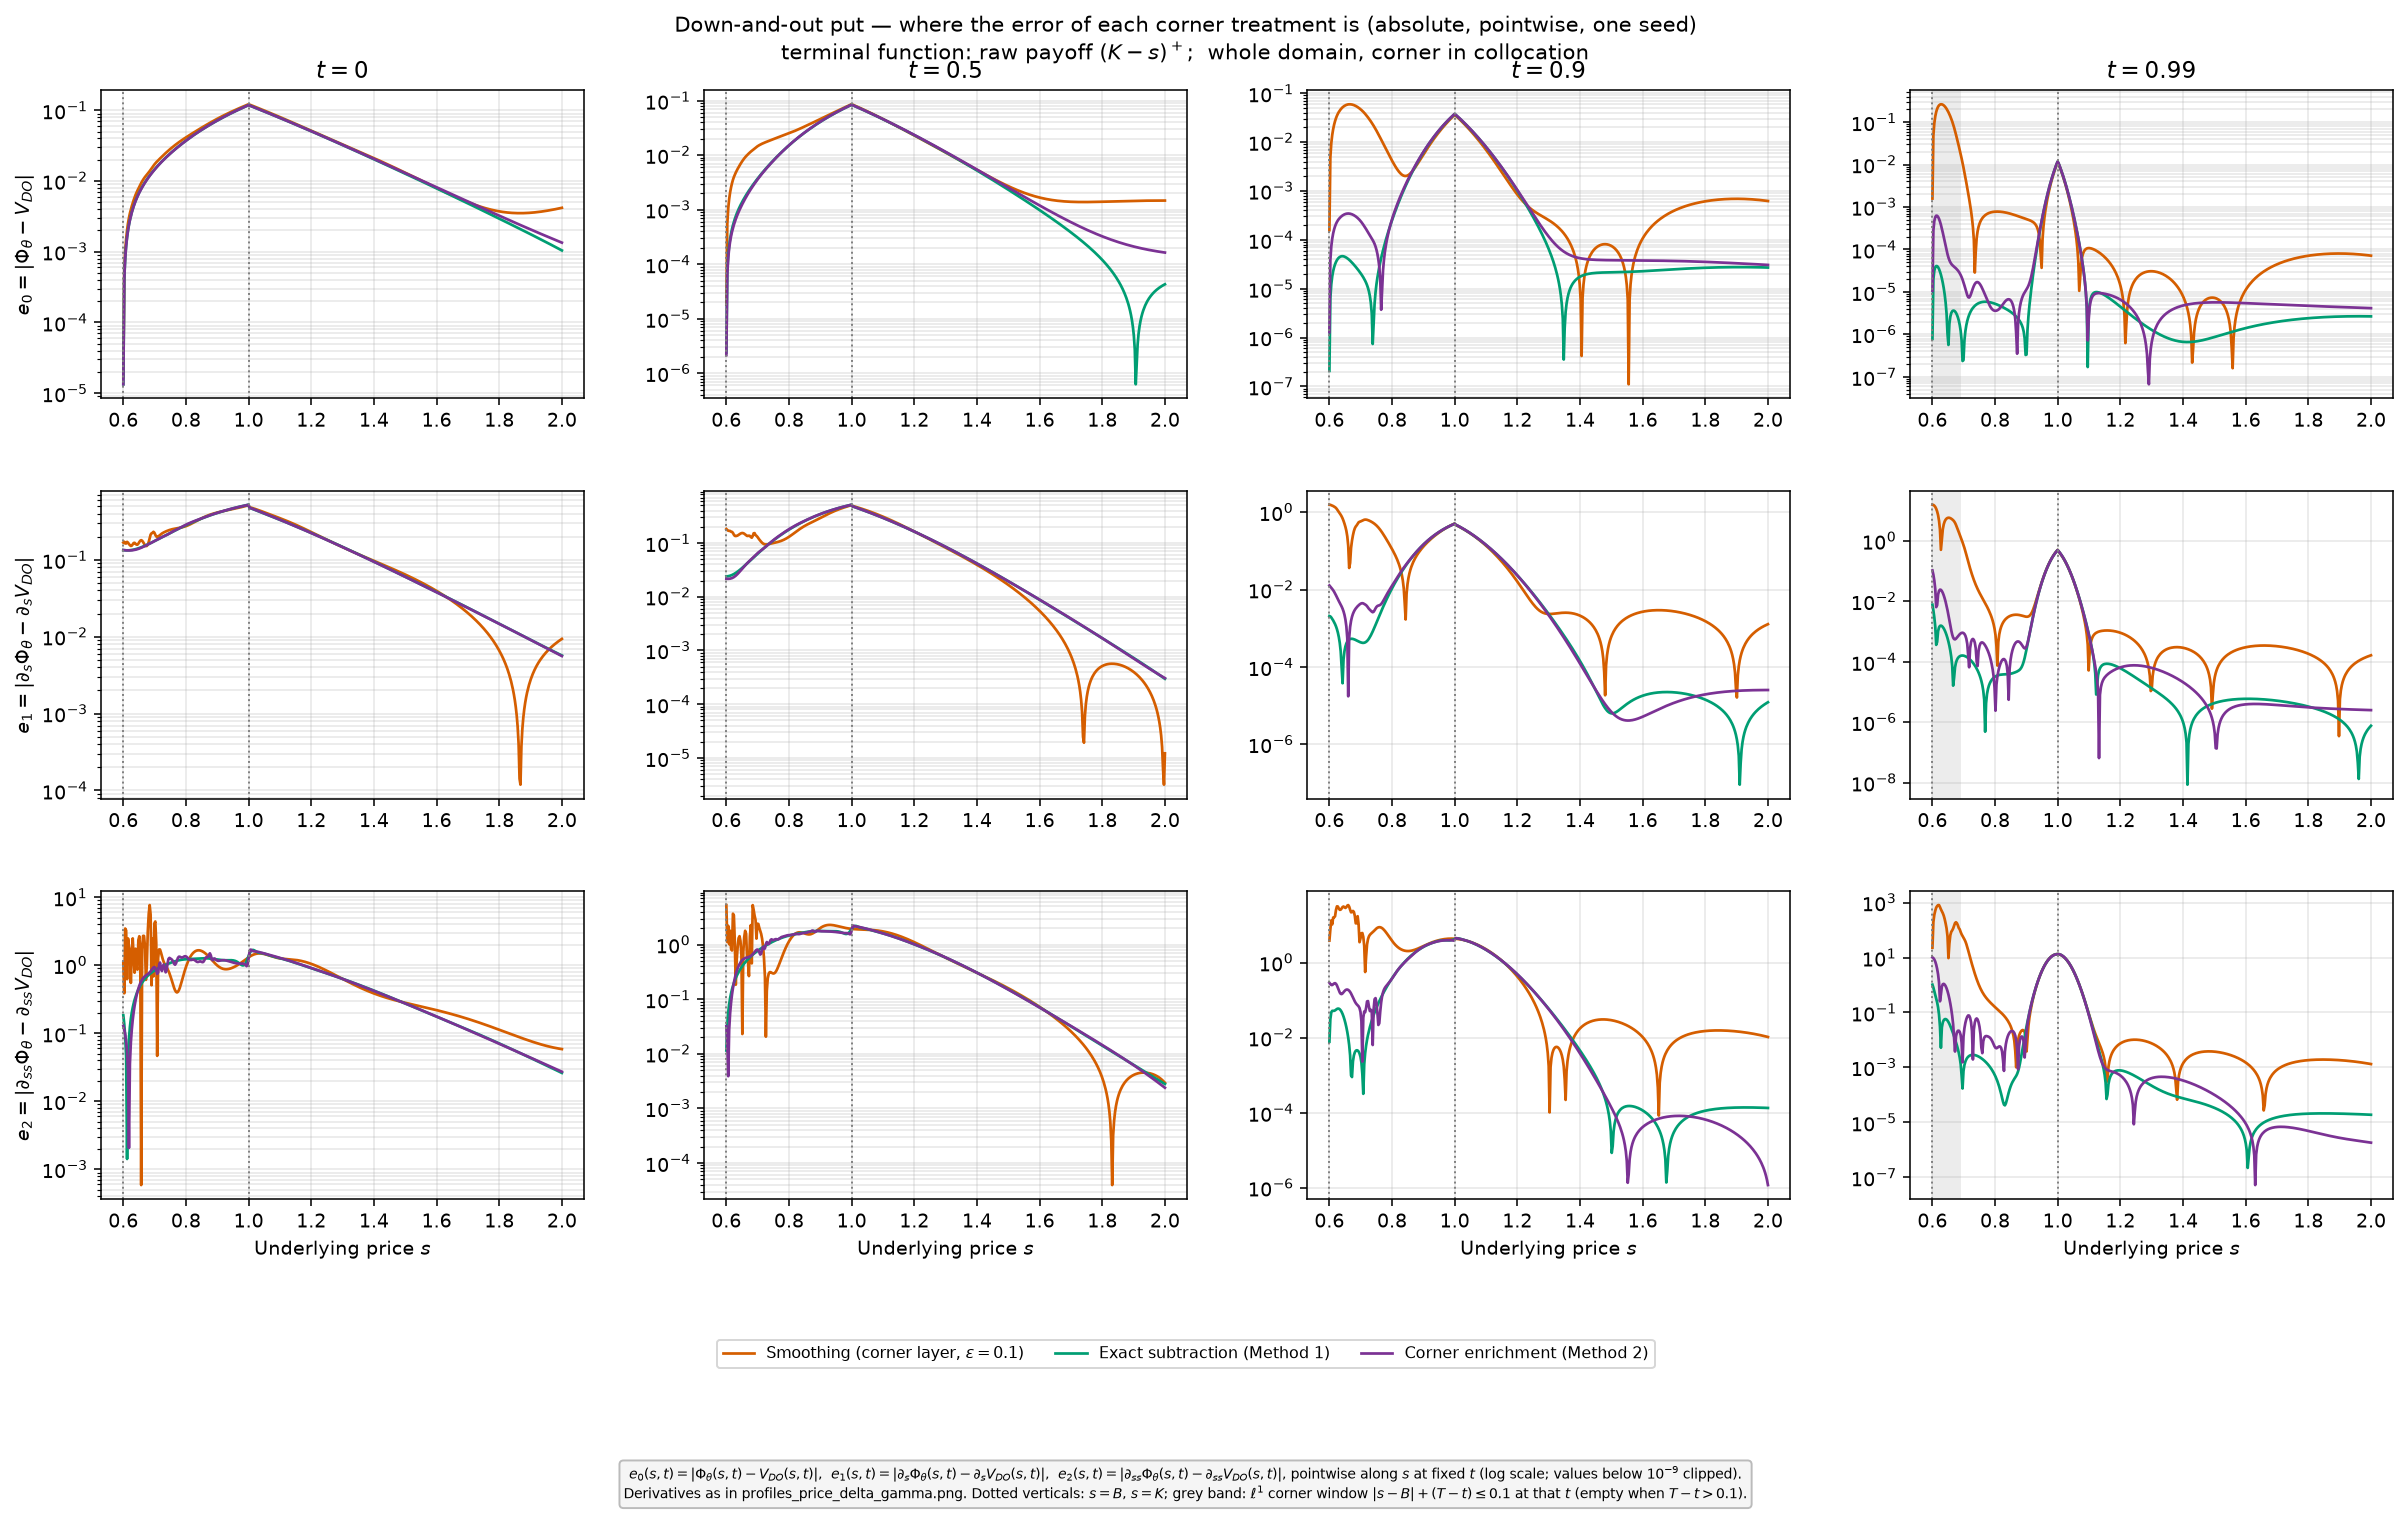
\includegraphics[width=\linewidth,height=0.8\textheight,keepaspectratio]{figures/absolute_errors_along_s_raw.png}
\caption{Erreurs absolues ponctuelles le long de $s$ : $e_0=|\Phi_\theta-V_{DO}|$, $e_1=|\partial_s\Phi_\theta-\partial_sV_{DO}|$, $e_2=|\partial_{ss}\Phi_\theta-\partial_{ss}V_{DO}|$ (échelle log). C'est la figure qui localise la valeur ajoutée des traitements analytiques. Les erreurs relatives par bande grandissent avec $s$ pour toutes les configurations parce que $V_{DO}\to0$, pas parce que l'erreur absolue grandit.}
\label{fig:abs-errors_raw}
\end{figure}

\end{landscape}

\begin{figure}[H]
\centering
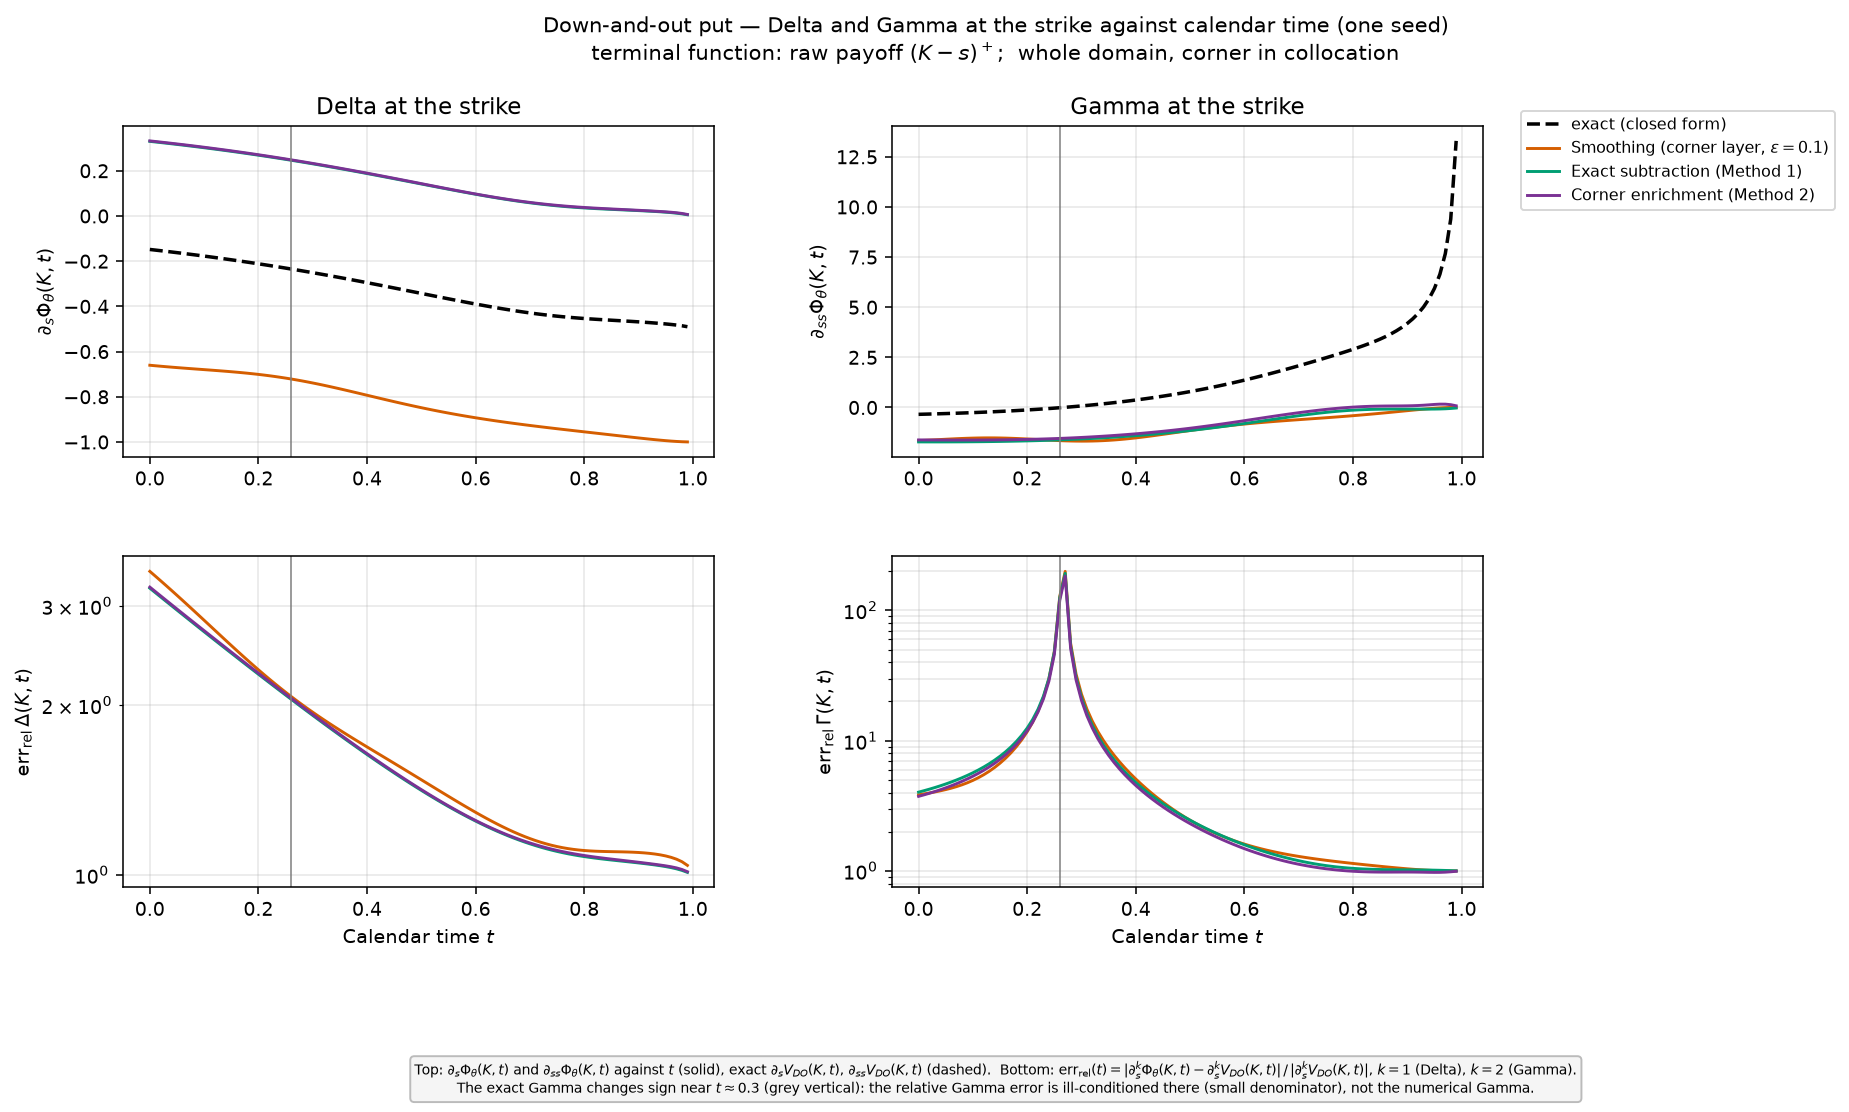
\includegraphics[width=0.95\linewidth]{figures/greeks_at_strike_vs_time_raw.png}
\caption{Haut : $\partial_s\Phi_\theta(K,t)$ et $\partial_{ss}\Phi_\theta(K,t)$ en fonction de $t$ (traits pleins), valeurs exactes en tirets. Bas : $\mathrm{err}_{\mathrm{rel}}\,\Delta(t)$ et $\mathrm{err}_{\mathrm{rel}}\,\Gamma(t)$ (échelle log). La verticale grise marque le zéro de $\partial_{ss}V_{DO}(K,\cdot)$, où l'erreur relative est mal conditionnée.}
\label{fig:greeks-vs-t_raw}
\end{figure}

\subsection{Fonction terminale : prix Black-Scholes du put (route autograd ordinaire)}
Source : \path{data/compare_corner_treatments_profiles/20260924_wholedomain_blackscholes}.
\begin{landscape}
\begin{figure}[H]
\centering
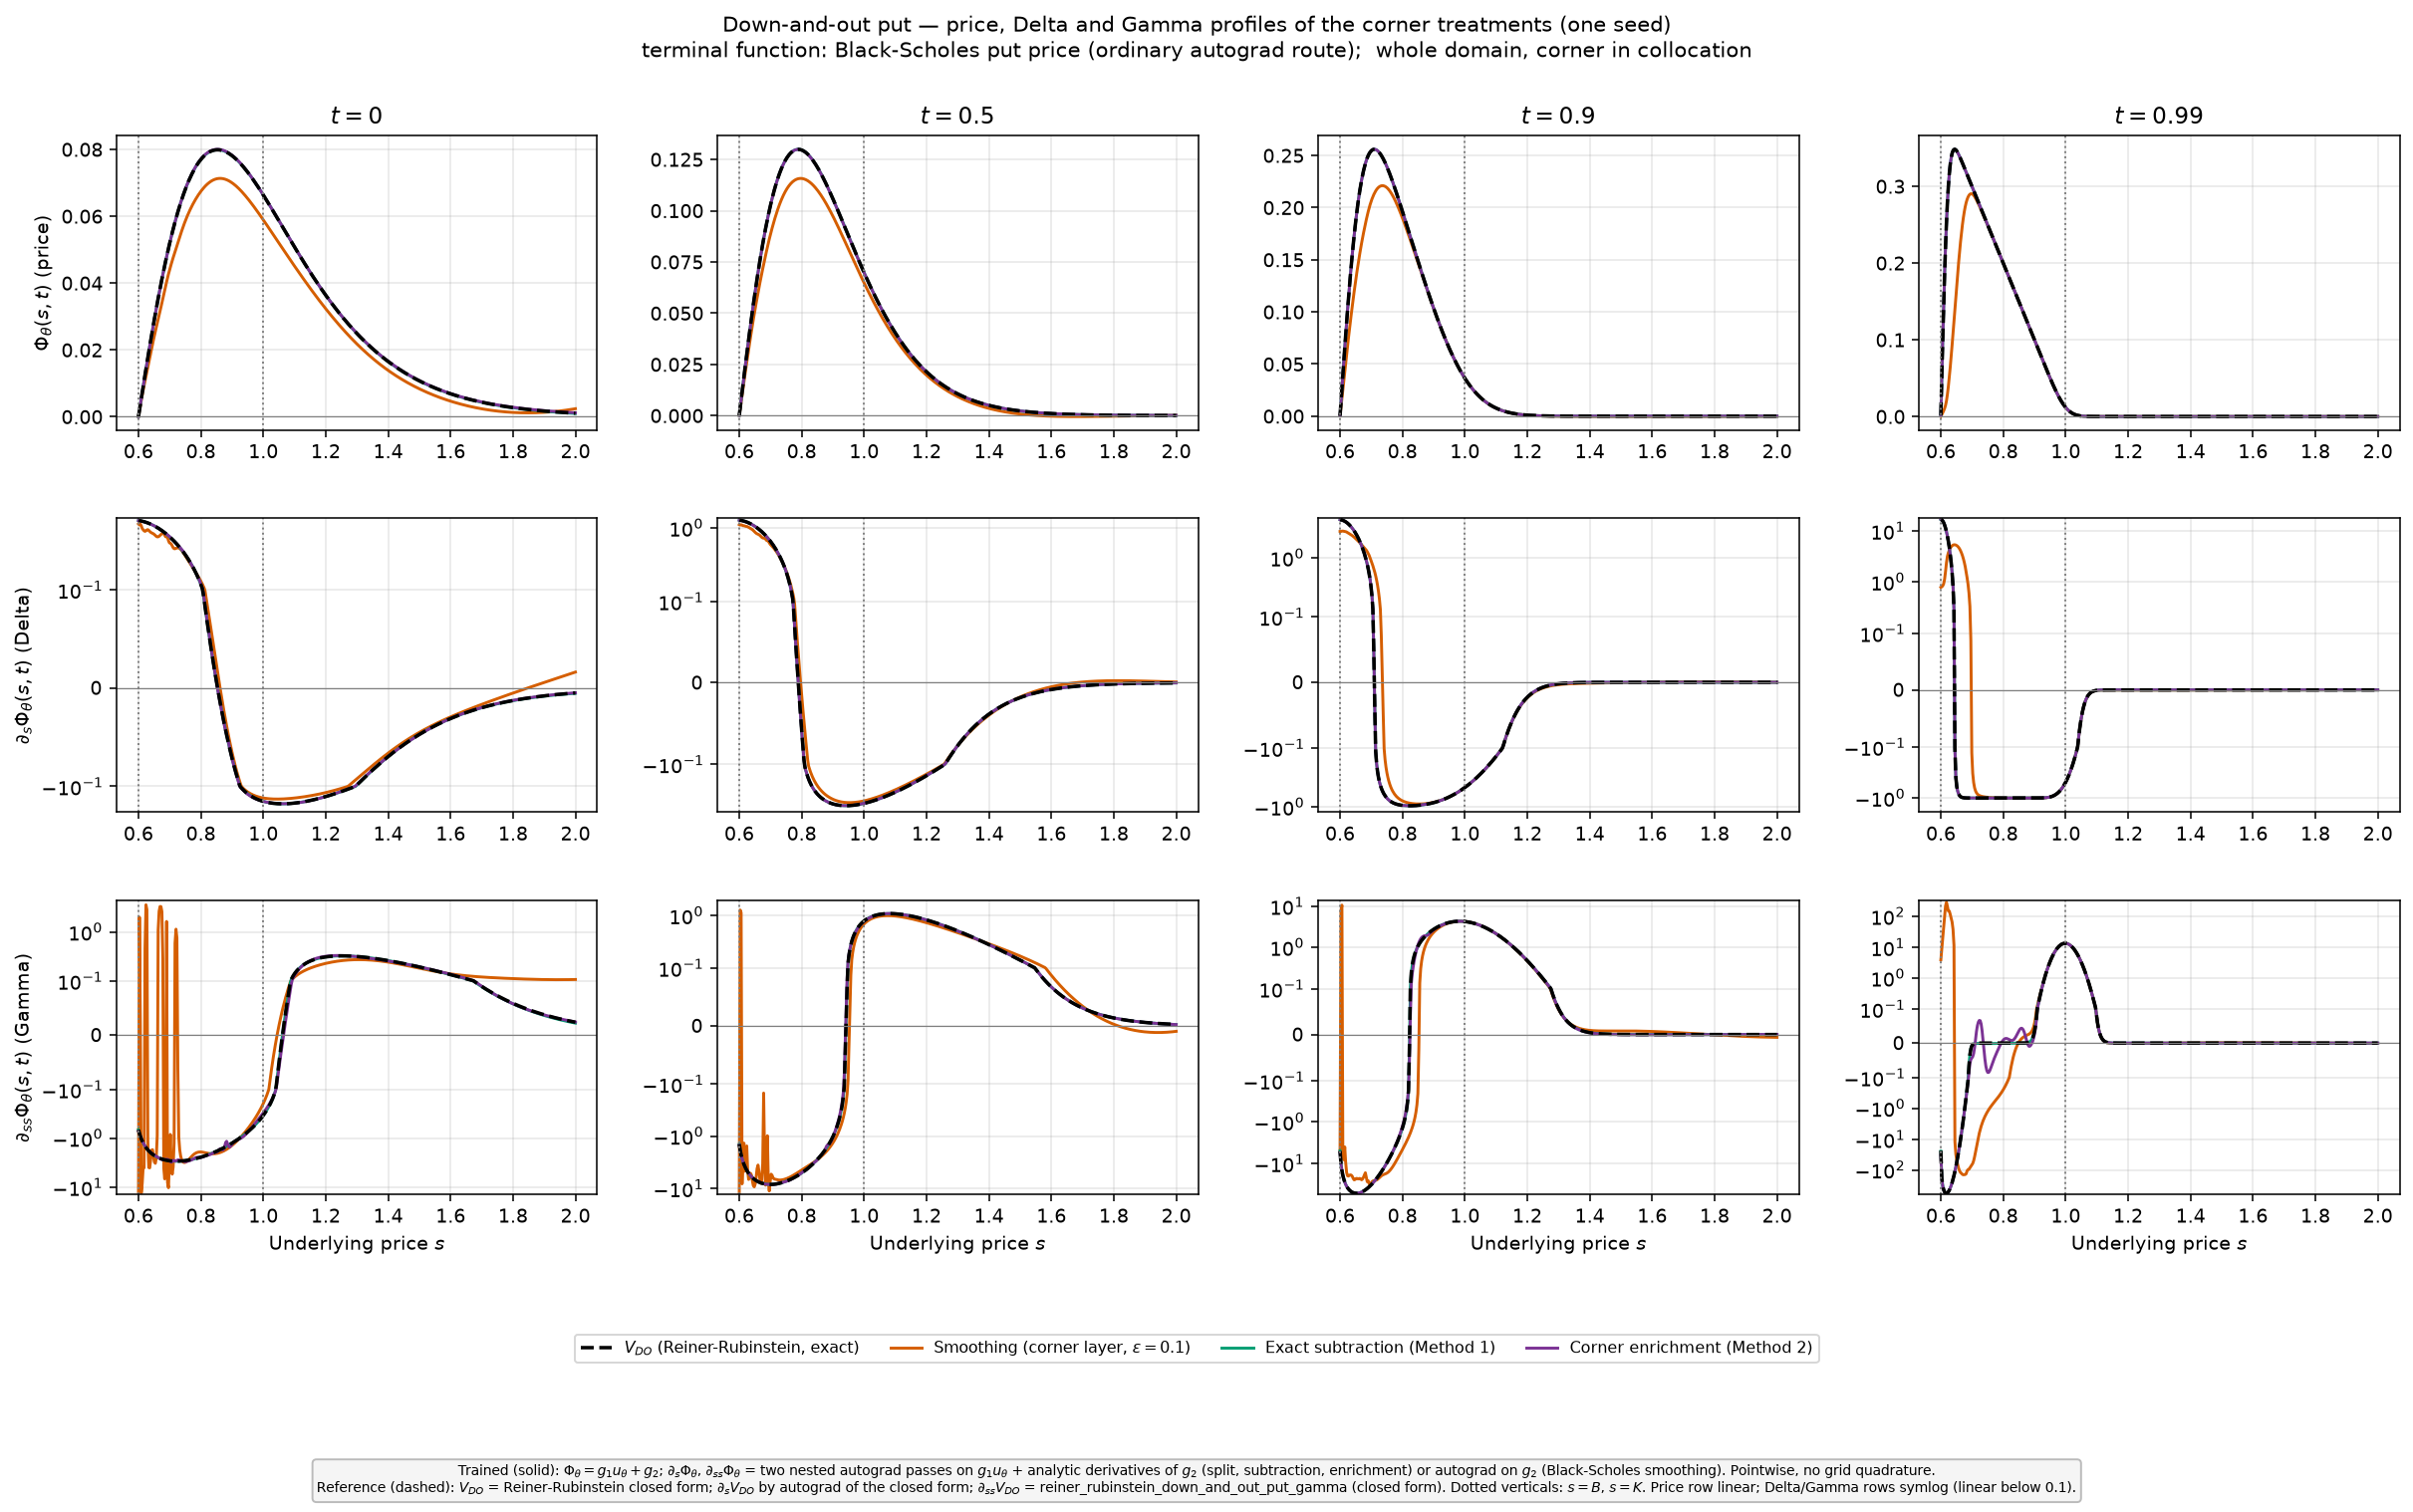
\includegraphics[width=\linewidth,height=0.8\textheight,keepaspectratio]{figures/profiles_price_delta_gamma_blackscholes.png}
\caption{Lignes : $\Phi_\theta(s,t)$, $\partial_s\Phi_\theta(s,t)$, $\partial_{ss}\Phi_\theta(s,t)$ ; colonnes : $t\in\{0,0.5,0.9,0.99\}$ ; forme fermée en tirets noirs. Prix en échelle linéaire ; $\Delta$ et $\Gamma$ en échelle symlog (linéaire sous $0.1$, logarithmique au-delà, des deux côtés de zéro).}
\label{fig:profiles_blackscholes}
\end{figure}

\end{landscape}

\begin{landscape}
\begin{figure}[H]
\centering
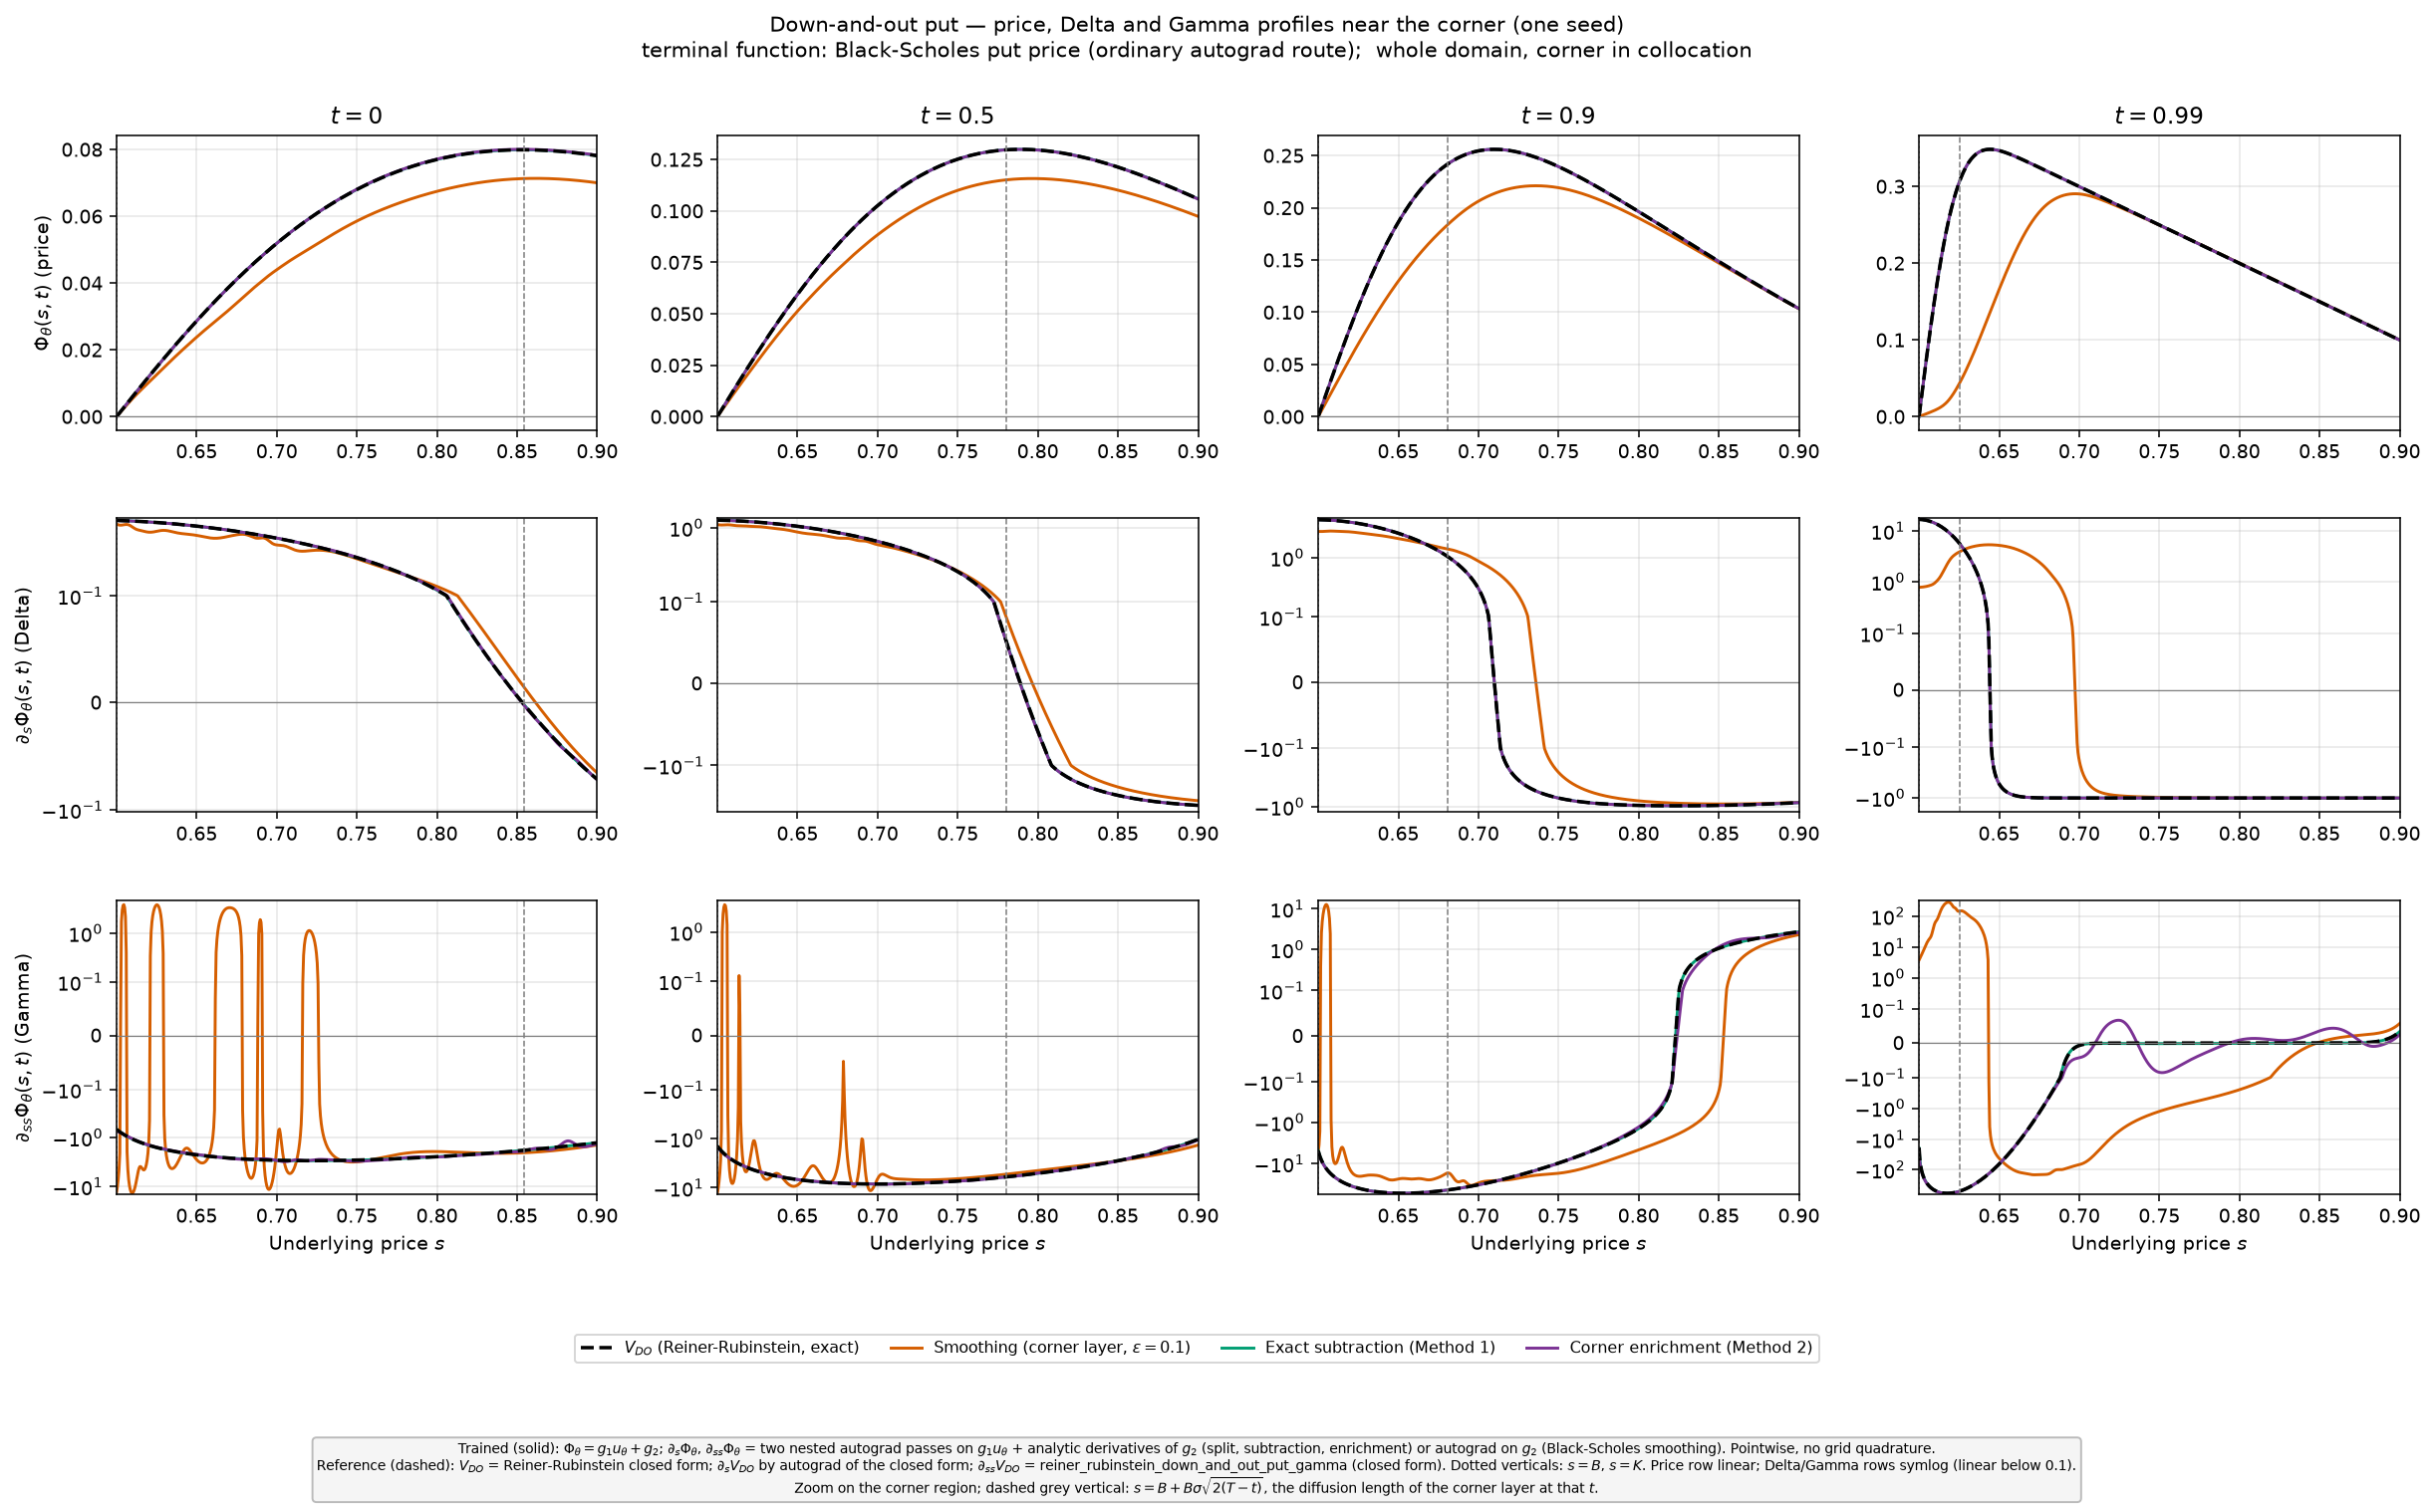
\includegraphics[width=\linewidth,height=0.8\textheight,keepaspectratio]{figures/profiles_price_delta_gamma_corner_zoom_blackscholes.png}
\caption{Même figure, restreinte à la région du coin $s\in(B, B+0.3)$ et évaluée sur sa propre grille dense (600 points, pas $5\times10^{-4}$). Tirets gris verticaux : $s=B+B\sigma\sqrt{2(T-t)}$, la longueur de diffusion de la couche de coin à ce $t$. Les ondulations de $\partial_{ss}\Phi_\theta$ du run de lissage (orange) sont confinées à la bande de transition du cutoff $\zeta((s-B)/\varepsilon)$, $s\in[0.6,0.7]$ : c'est la courbure de $\zeta$ ($\zeta''\sim\varepsilon^{-2}$) que le réseau n'annule pas. La soustraction (vert) est confondue avec la forme fermée sur les trois lignes ; l'enrichissement (violet) l'est aussi hors de la bande de transition de $\chi$, $[0.7,0.9]$.}
\label{fig:profiles-zoom_blackscholes}
\end{figure}

\end{landscape}

\begin{landscape}
\begin{figure}[H]
\centering
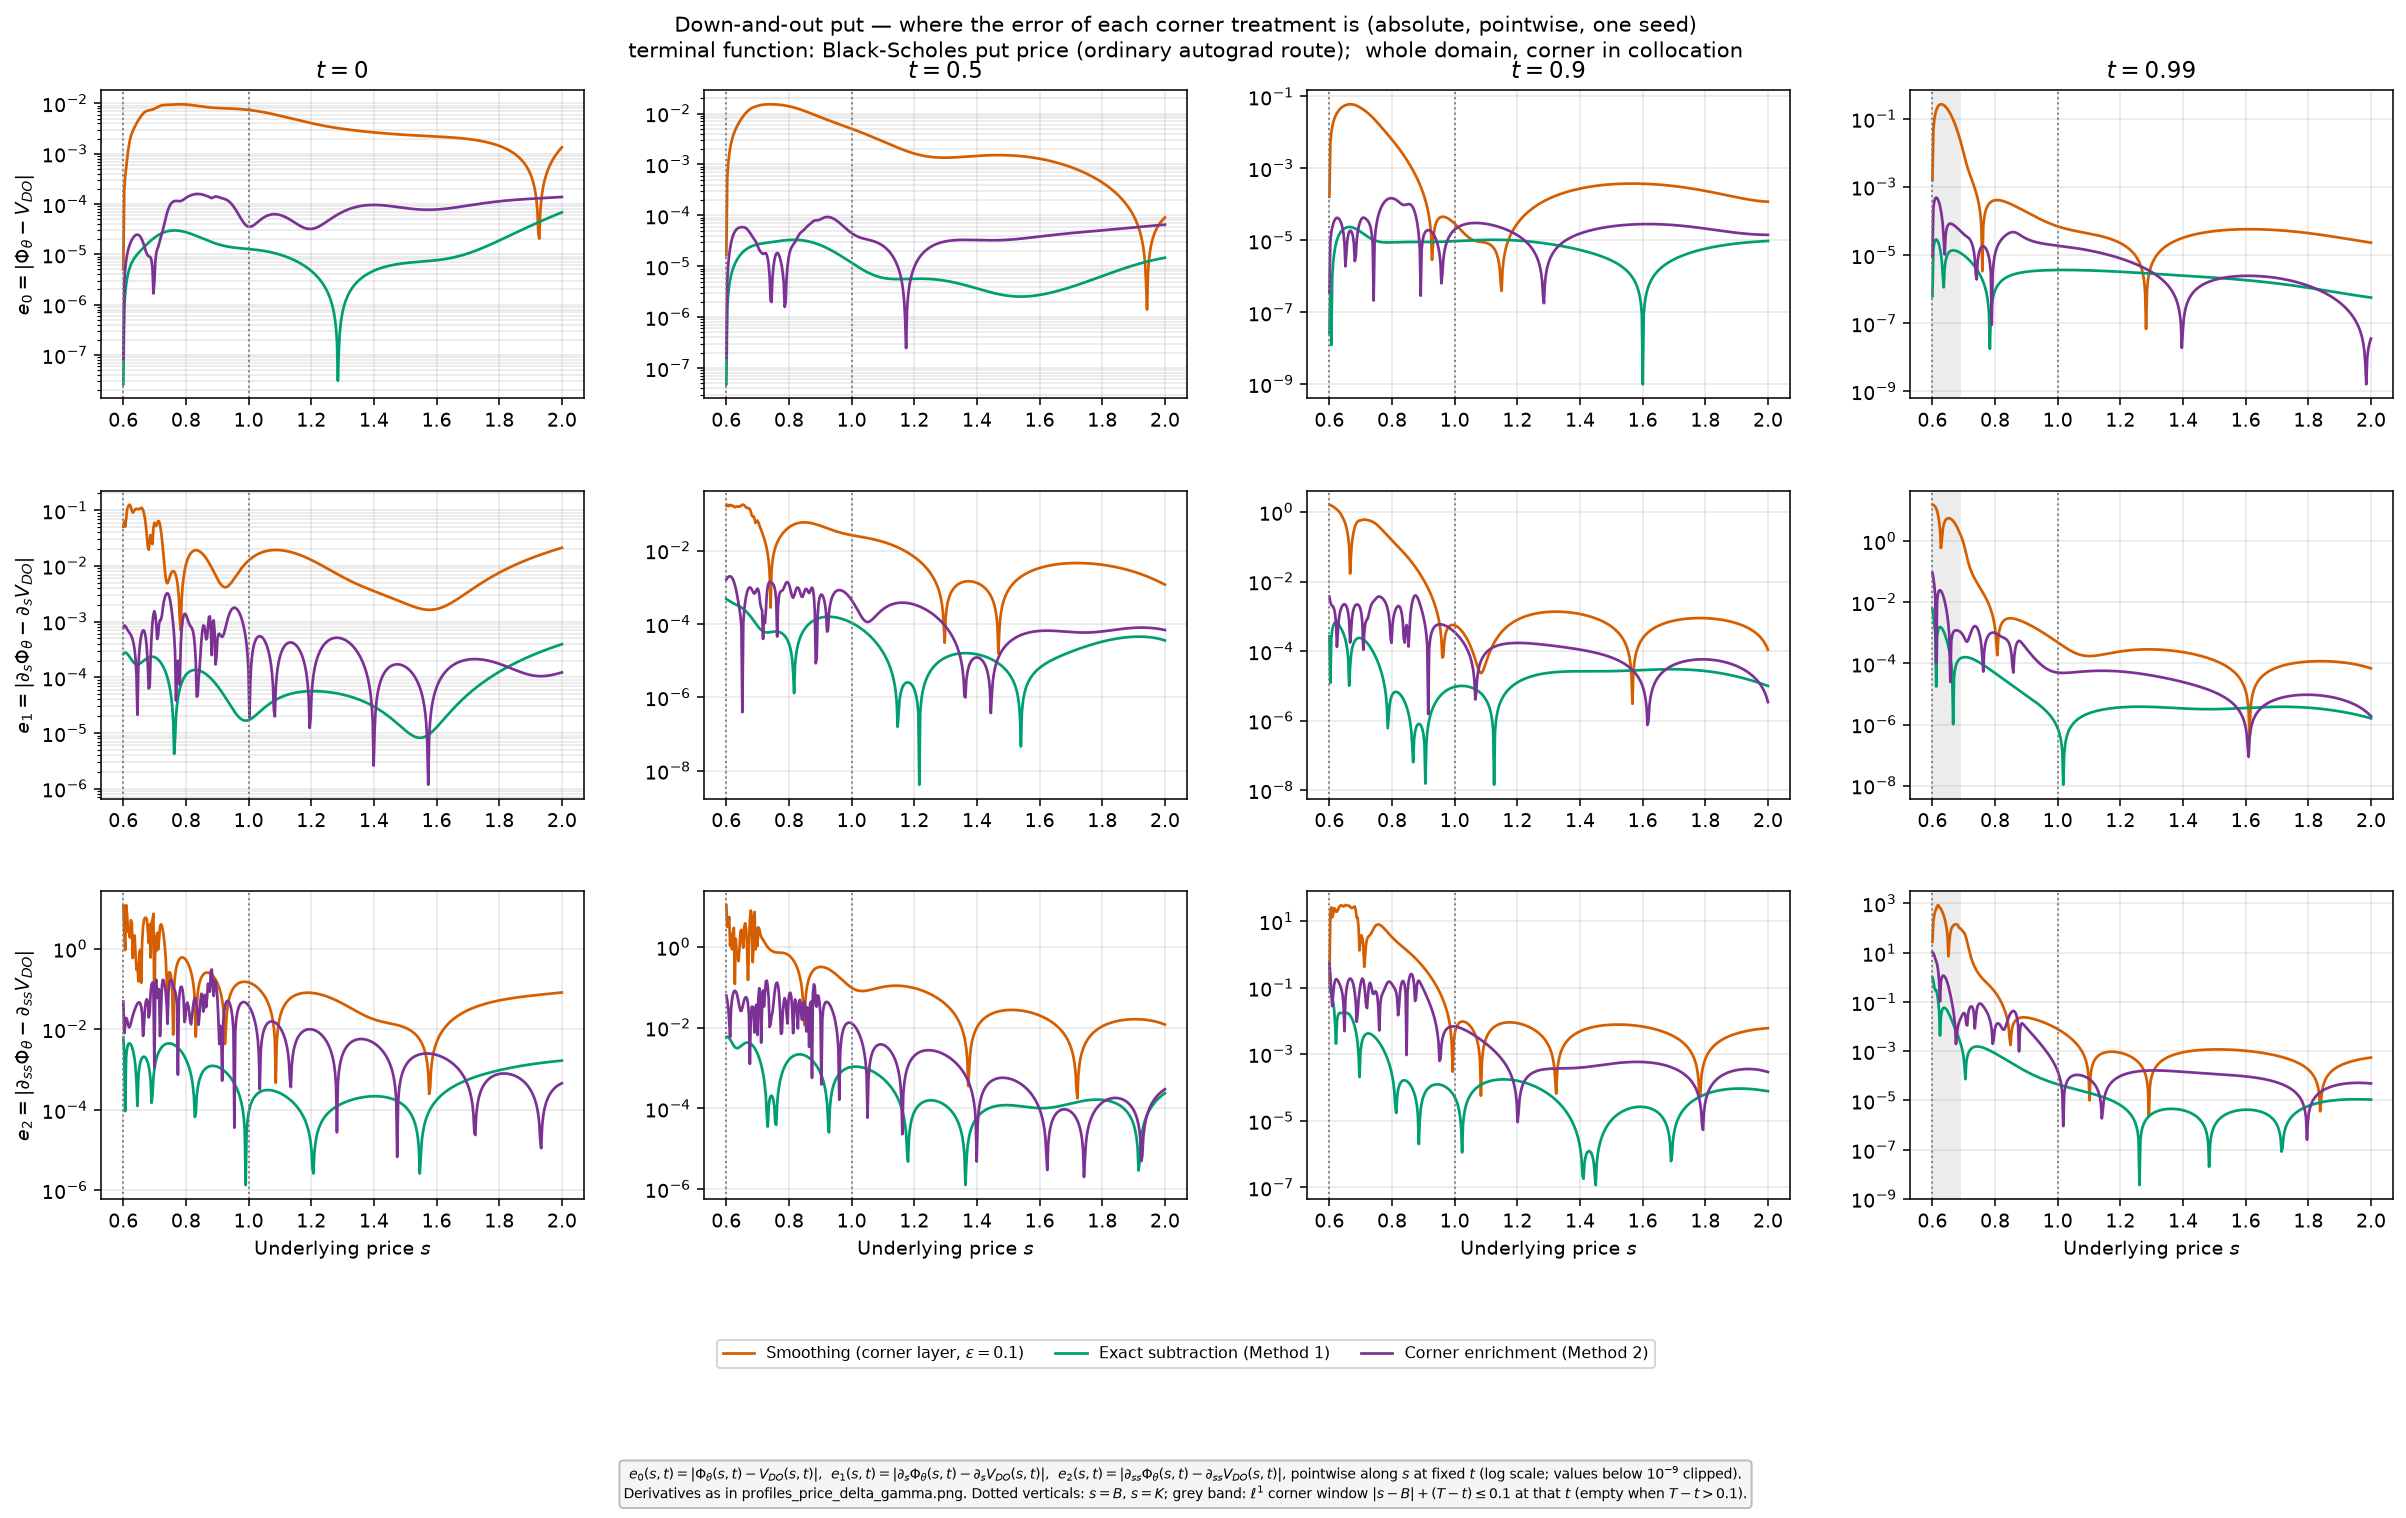
\includegraphics[width=\linewidth,height=0.8\textheight,keepaspectratio]{figures/absolute_errors_along_s_blackscholes.png}
\caption{Erreurs absolues ponctuelles le long de $s$ : $e_0=|\Phi_\theta-V_{DO}|$, $e_1=|\partial_s\Phi_\theta-\partial_sV_{DO}|$, $e_2=|\partial_{ss}\Phi_\theta-\partial_{ss}V_{DO}|$ (échelle log). C'est la figure qui localise la valeur ajoutée des traitements analytiques. Les erreurs relatives par bande grandissent avec $s$ pour toutes les configurations parce que $V_{DO}\to0$, pas parce que l'erreur absolue grandit.}
\label{fig:abs-errors_blackscholes}
\end{figure}

\end{landscape}

\begin{figure}[H]
\centering
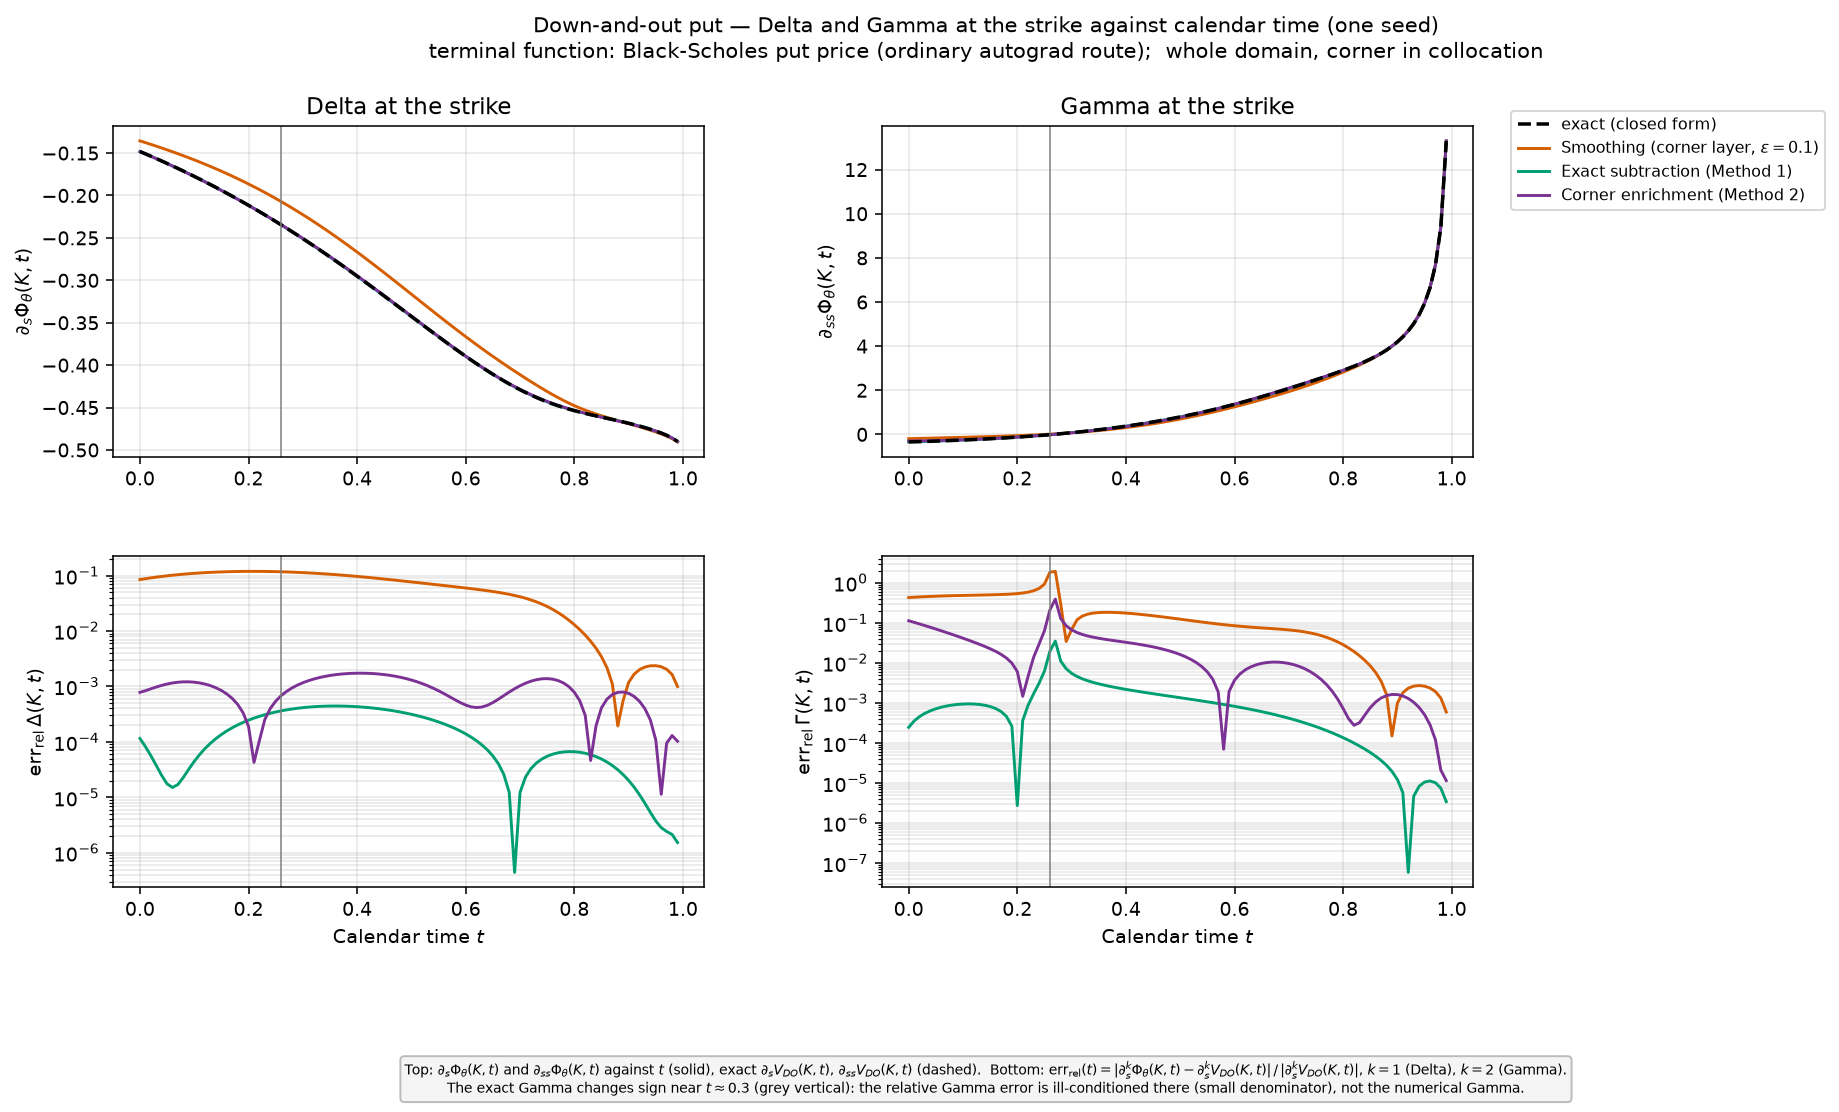
\includegraphics[width=0.95\linewidth]{figures/greeks_at_strike_vs_time_blackscholes.png}
\caption{Haut : $\partial_s\Phi_\theta(K,t)$ et $\partial_{ss}\Phi_\theta(K,t)$ en fonction de $t$ (traits pleins), valeurs exactes en tirets. Bas : $\mathrm{err}_{\mathrm{rel}}\,\Delta(t)$ et $\mathrm{err}_{\mathrm{rel}}\,\Gamma(t)$ (échelle log). La verticale grise marque le zéro de $\partial_{ss}V_{DO}(K,\cdot)$, où l'erreur relative est mal conditionnée.}
\label{fig:greeks-vs-t_blackscholes}
\end{figure}

\subsection{Fonction terminale : profil de semi-groupe scindé}
Source : \path{data/compare_corner_treatments_profiles/20260924_wholedomain_split}.
\begin{landscape}
\begin{figure}[H]
\centering
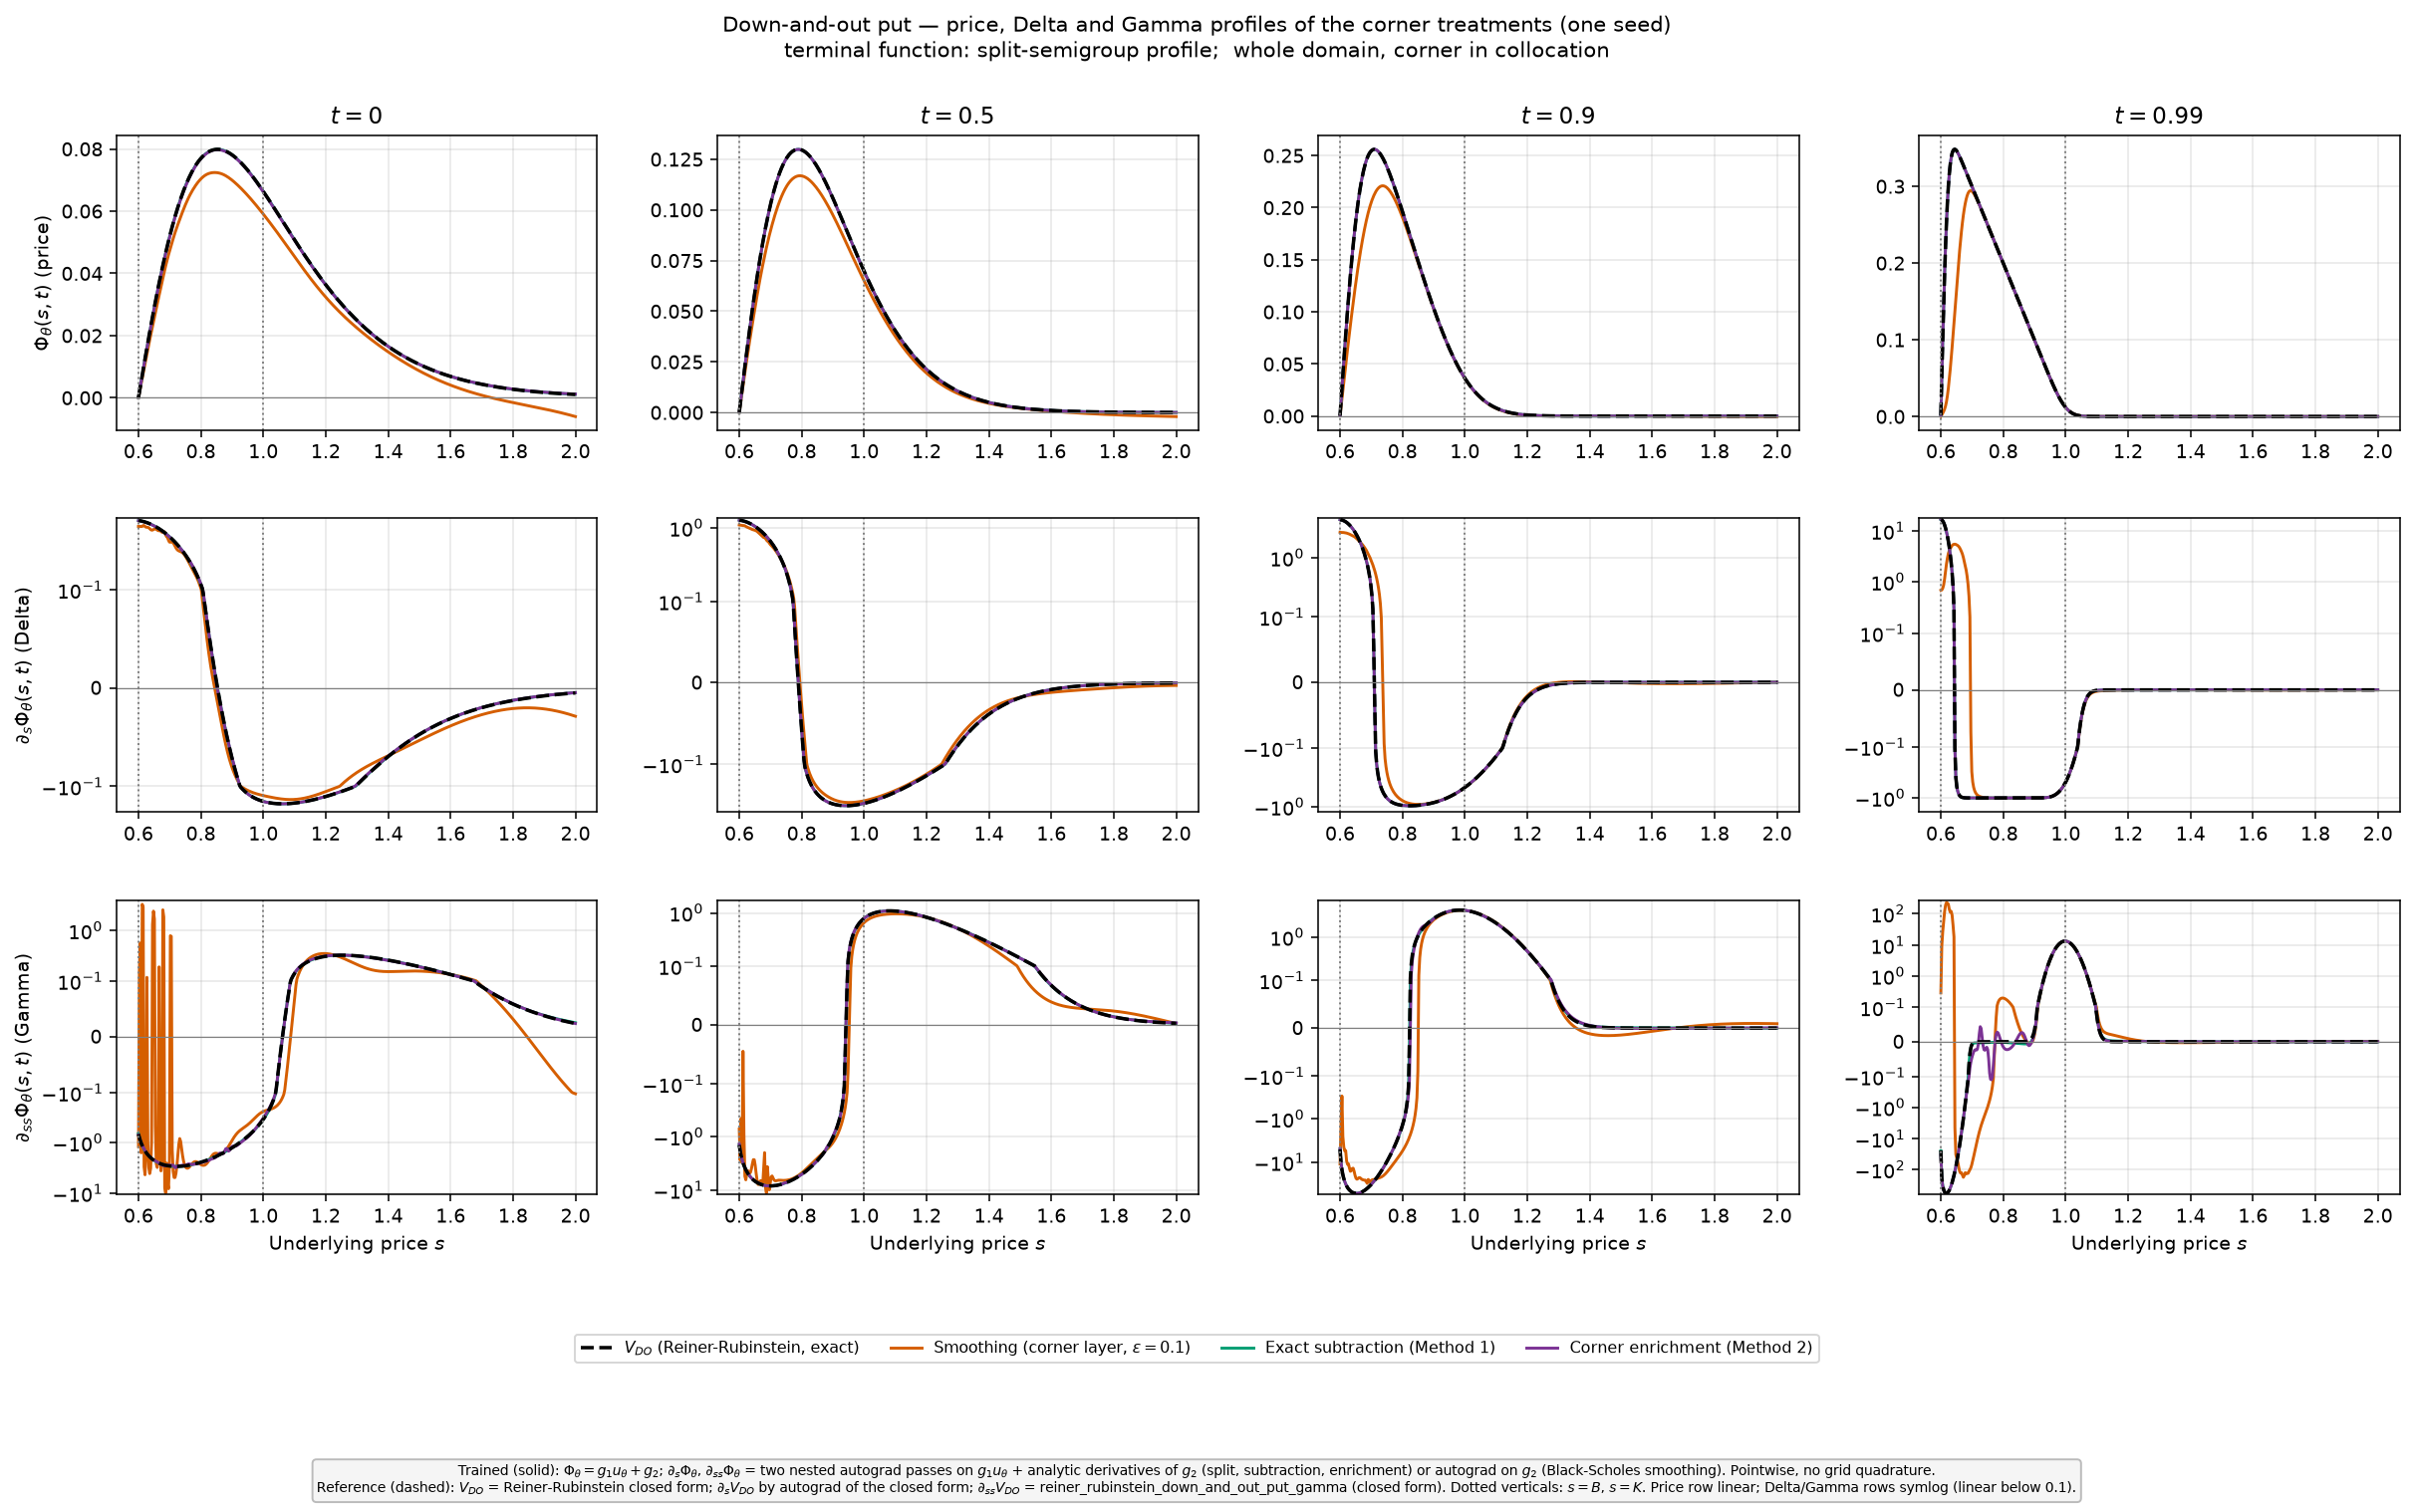
\includegraphics[width=\linewidth,height=0.8\textheight,keepaspectratio]{figures/profiles_price_delta_gamma_split.png}
\caption{Lignes : $\Phi_\theta(s,t)$, $\partial_s\Phi_\theta(s,t)$, $\partial_{ss}\Phi_\theta(s,t)$ ; colonnes : $t\in\{0,0.5,0.9,0.99\}$ ; forme fermée en tirets noirs. Prix en échelle linéaire ; $\Delta$ et $\Gamma$ en échelle symlog (linéaire sous $0.1$, logarithmique au-delà, des deux côtés de zéro).}
\label{fig:profiles_split}
\end{figure}

\end{landscape}

\begin{landscape}
\begin{figure}[H]
\centering
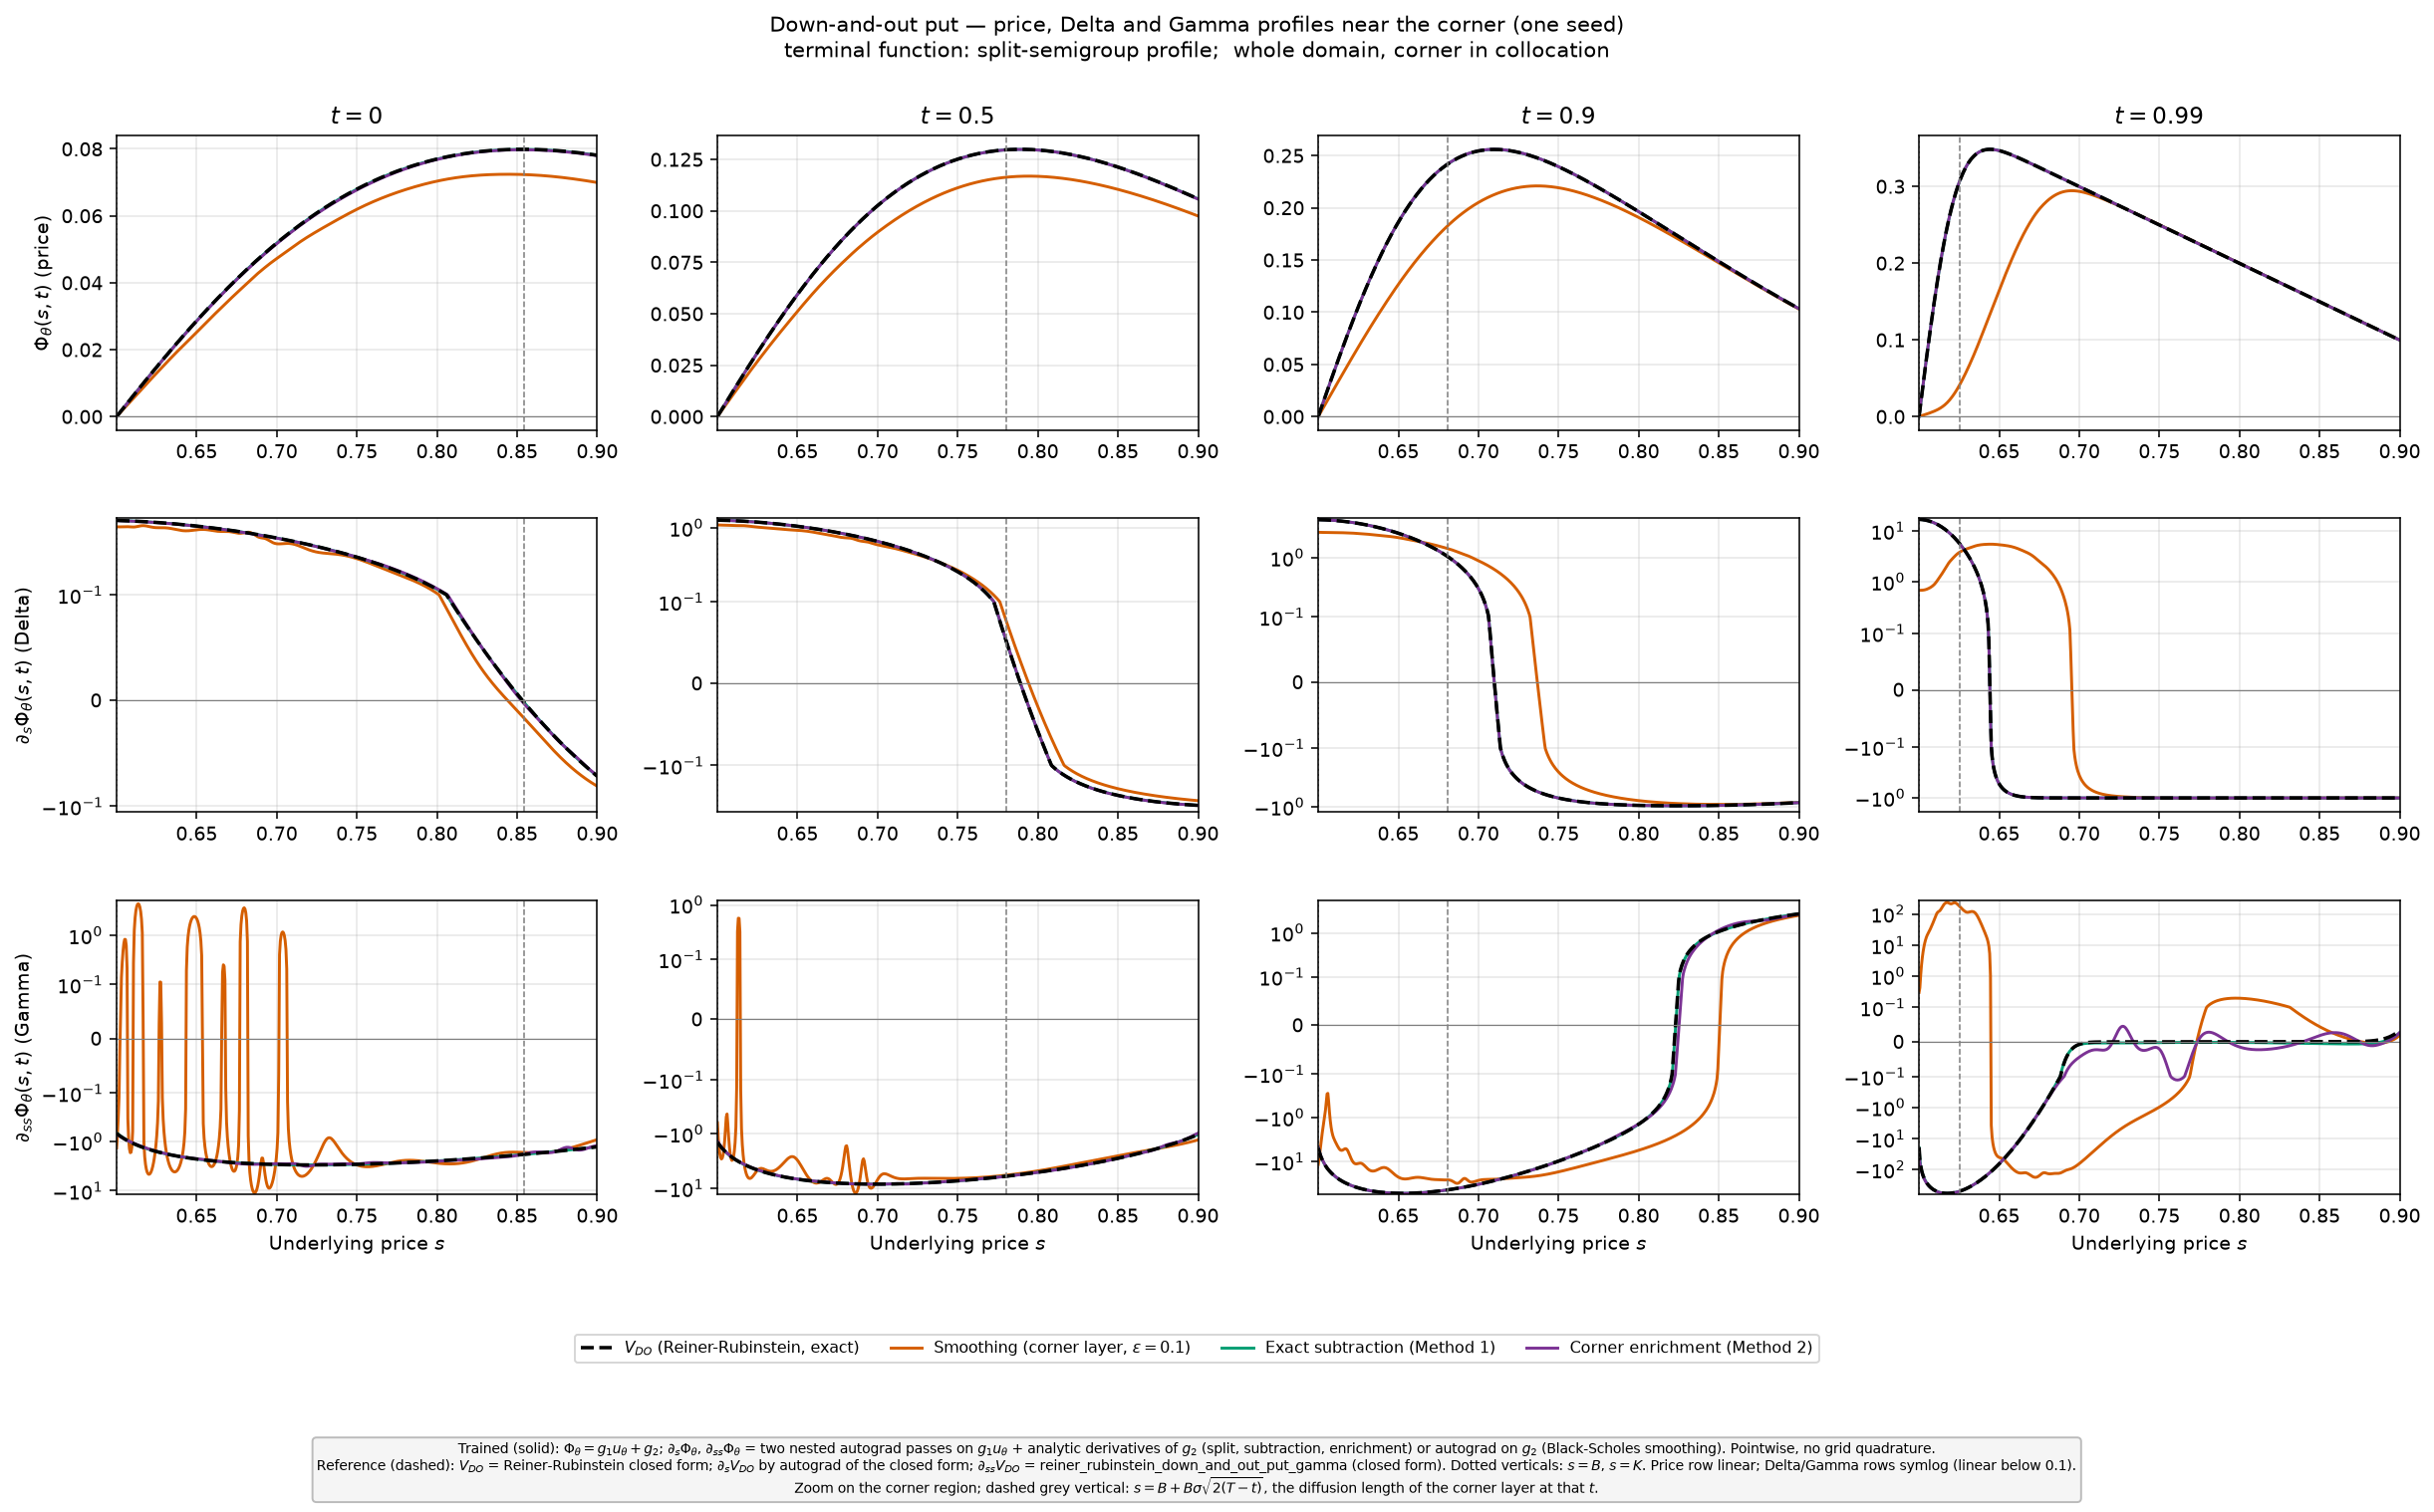
\includegraphics[width=\linewidth,height=0.8\textheight,keepaspectratio]{figures/profiles_price_delta_gamma_corner_zoom_split.png}
\caption{Même figure, restreinte à la région du coin $s\in(B, B+0.3)$ et évaluée sur sa propre grille dense (600 points, pas $5\times10^{-4}$). Tirets gris verticaux : $s=B+B\sigma\sqrt{2(T-t)}$, la longueur de diffusion de la couche de coin à ce $t$. Les ondulations de $\partial_{ss}\Phi_\theta$ du run de lissage (orange) sont confinées à la bande de transition du cutoff $\zeta((s-B)/\varepsilon)$, $s\in[0.6,0.7]$ : c'est la courbure de $\zeta$ ($\zeta''\sim\varepsilon^{-2}$) que le réseau n'annule pas. La soustraction (vert) est confondue avec la forme fermée sur les trois lignes ; l'enrichissement (violet) l'est aussi hors de la bande de transition de $\chi$, $[0.7,0.9]$.}
\label{fig:profiles-zoom_split}
\end{figure}

\end{landscape}

\begin{landscape}
\begin{figure}[H]
\centering
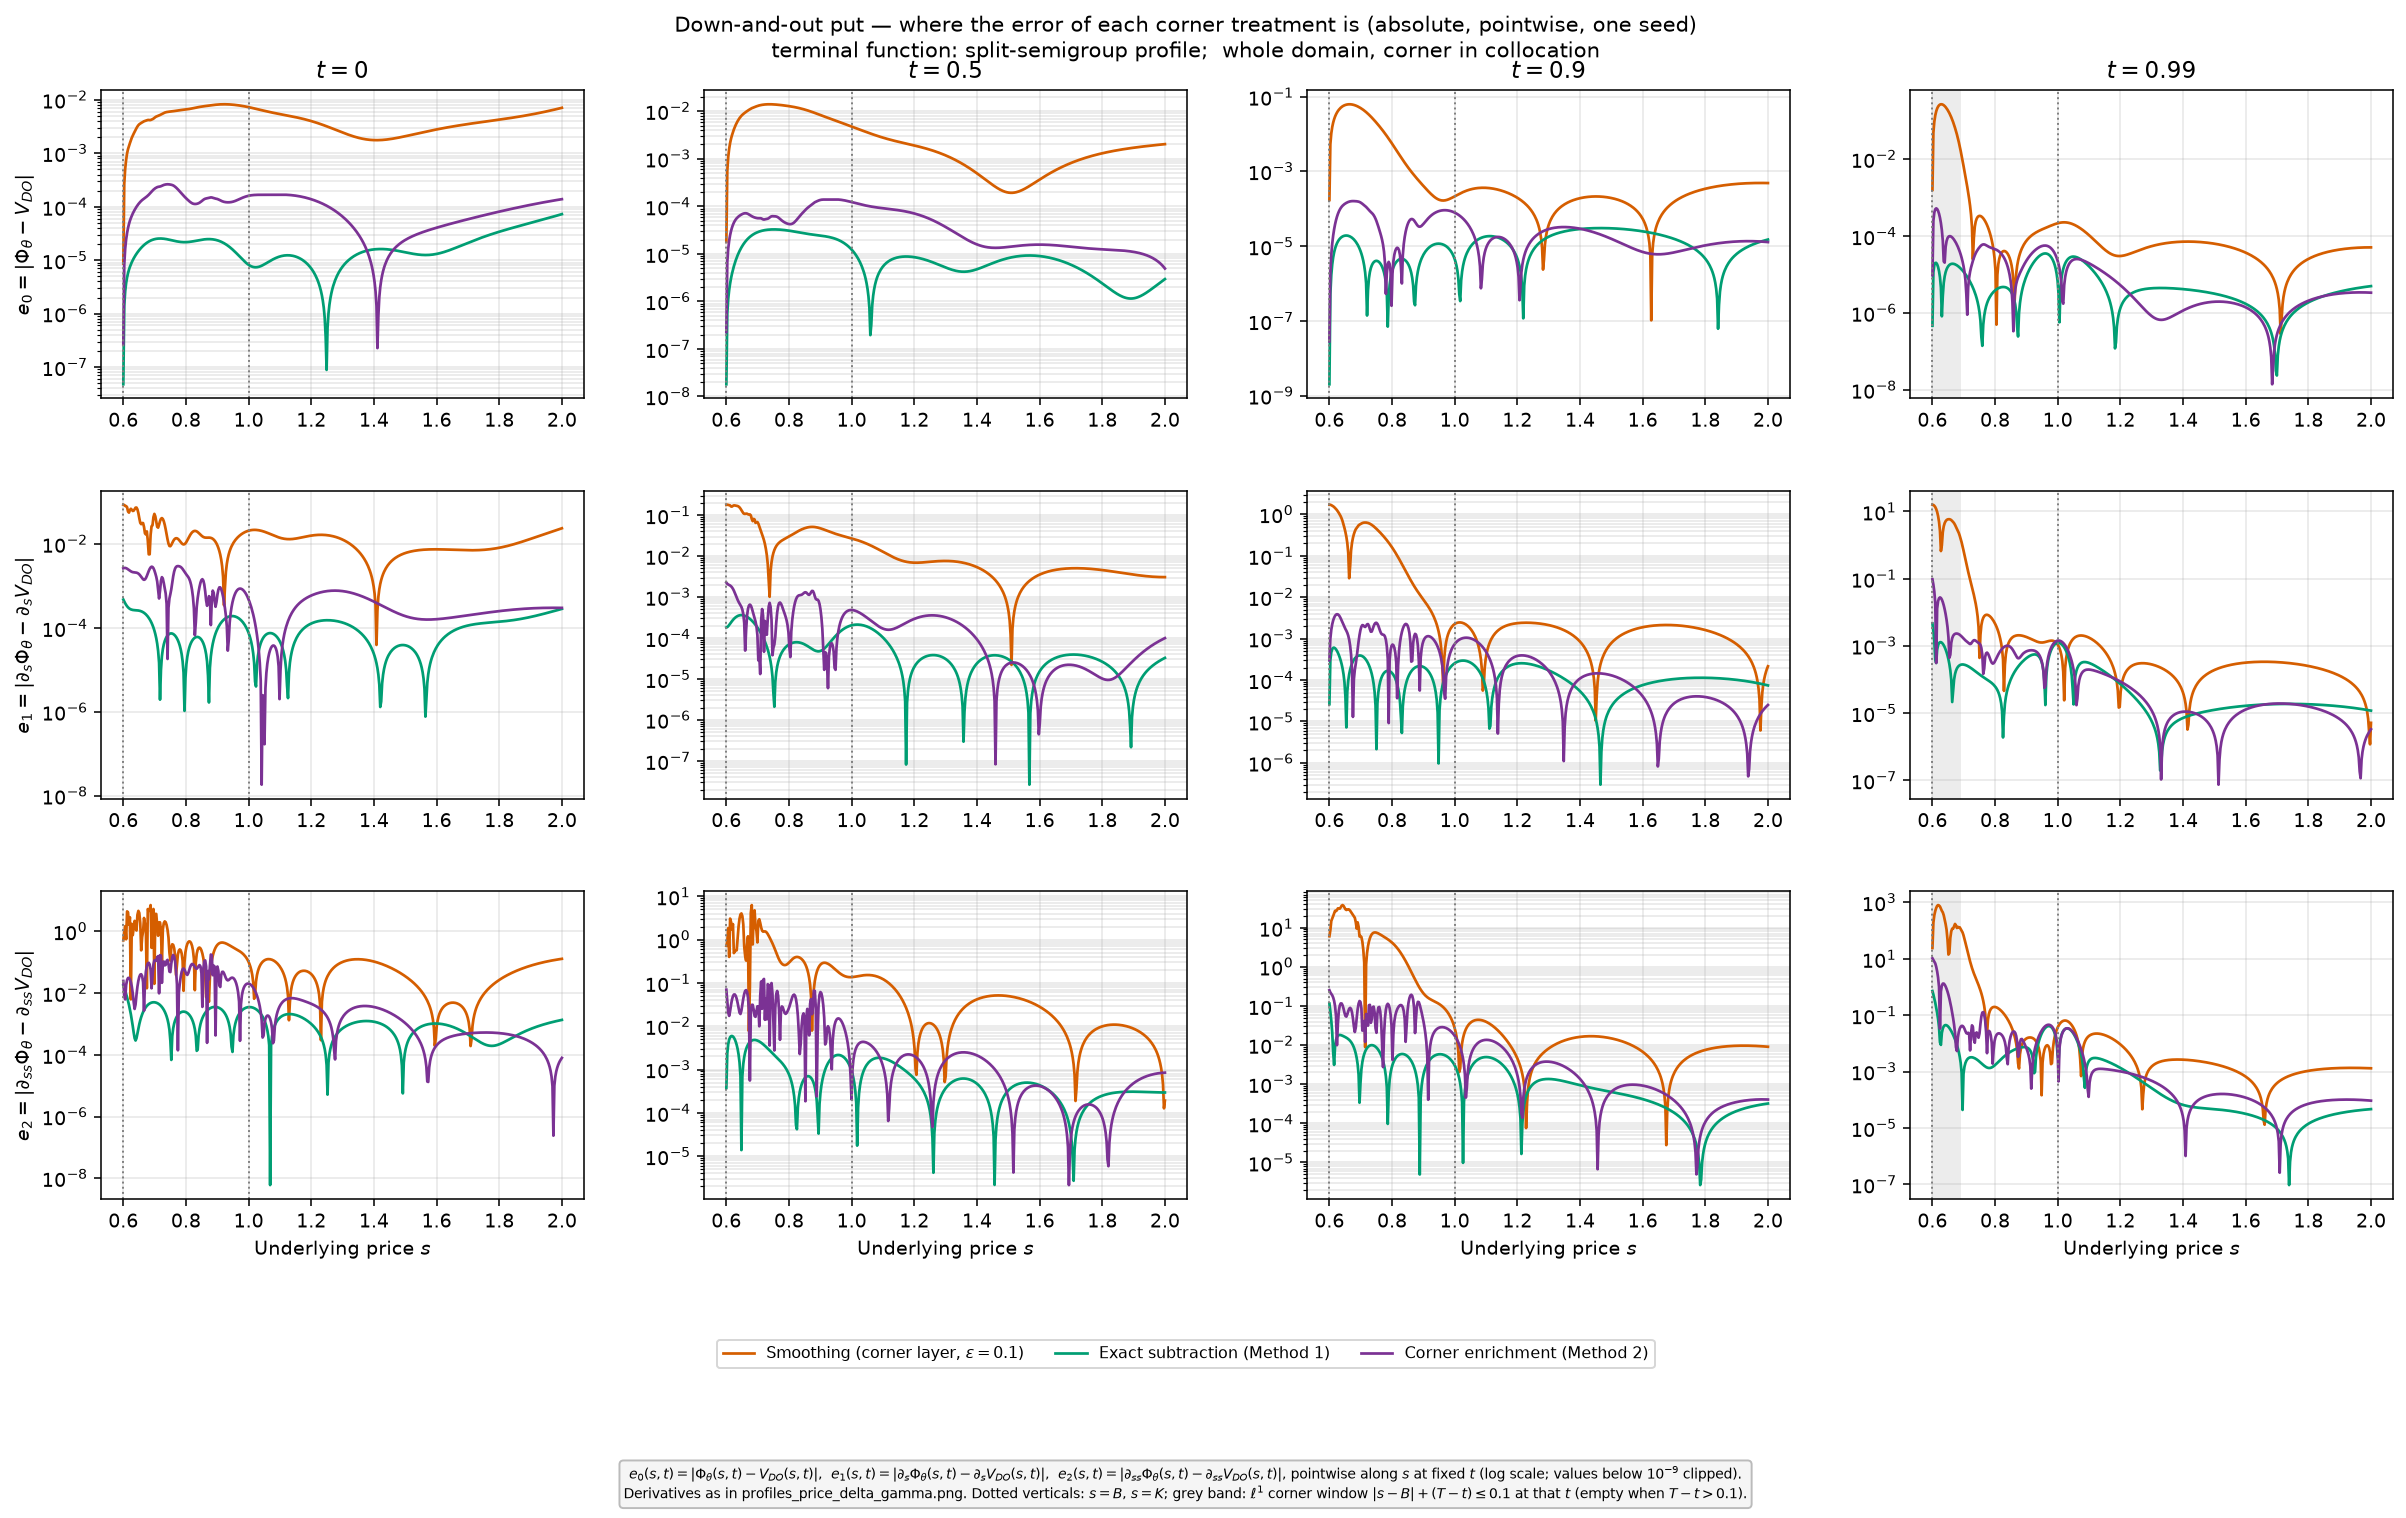
\includegraphics[width=\linewidth,height=0.8\textheight,keepaspectratio]{figures/absolute_errors_along_s_split.png}
\caption{Erreurs absolues ponctuelles le long de $s$ : $e_0=|\Phi_\theta-V_{DO}|$, $e_1=|\partial_s\Phi_\theta-\partial_sV_{DO}|$, $e_2=|\partial_{ss}\Phi_\theta-\partial_{ss}V_{DO}|$ (échelle log). C'est la figure qui localise la valeur ajoutée des traitements analytiques. Les erreurs relatives par bande grandissent avec $s$ pour toutes les configurations parce que $V_{DO}\to0$, pas parce que l'erreur absolue grandit.}
\label{fig:abs-errors_split}
\end{figure}

\end{landscape}

\begin{figure}[H]
\centering
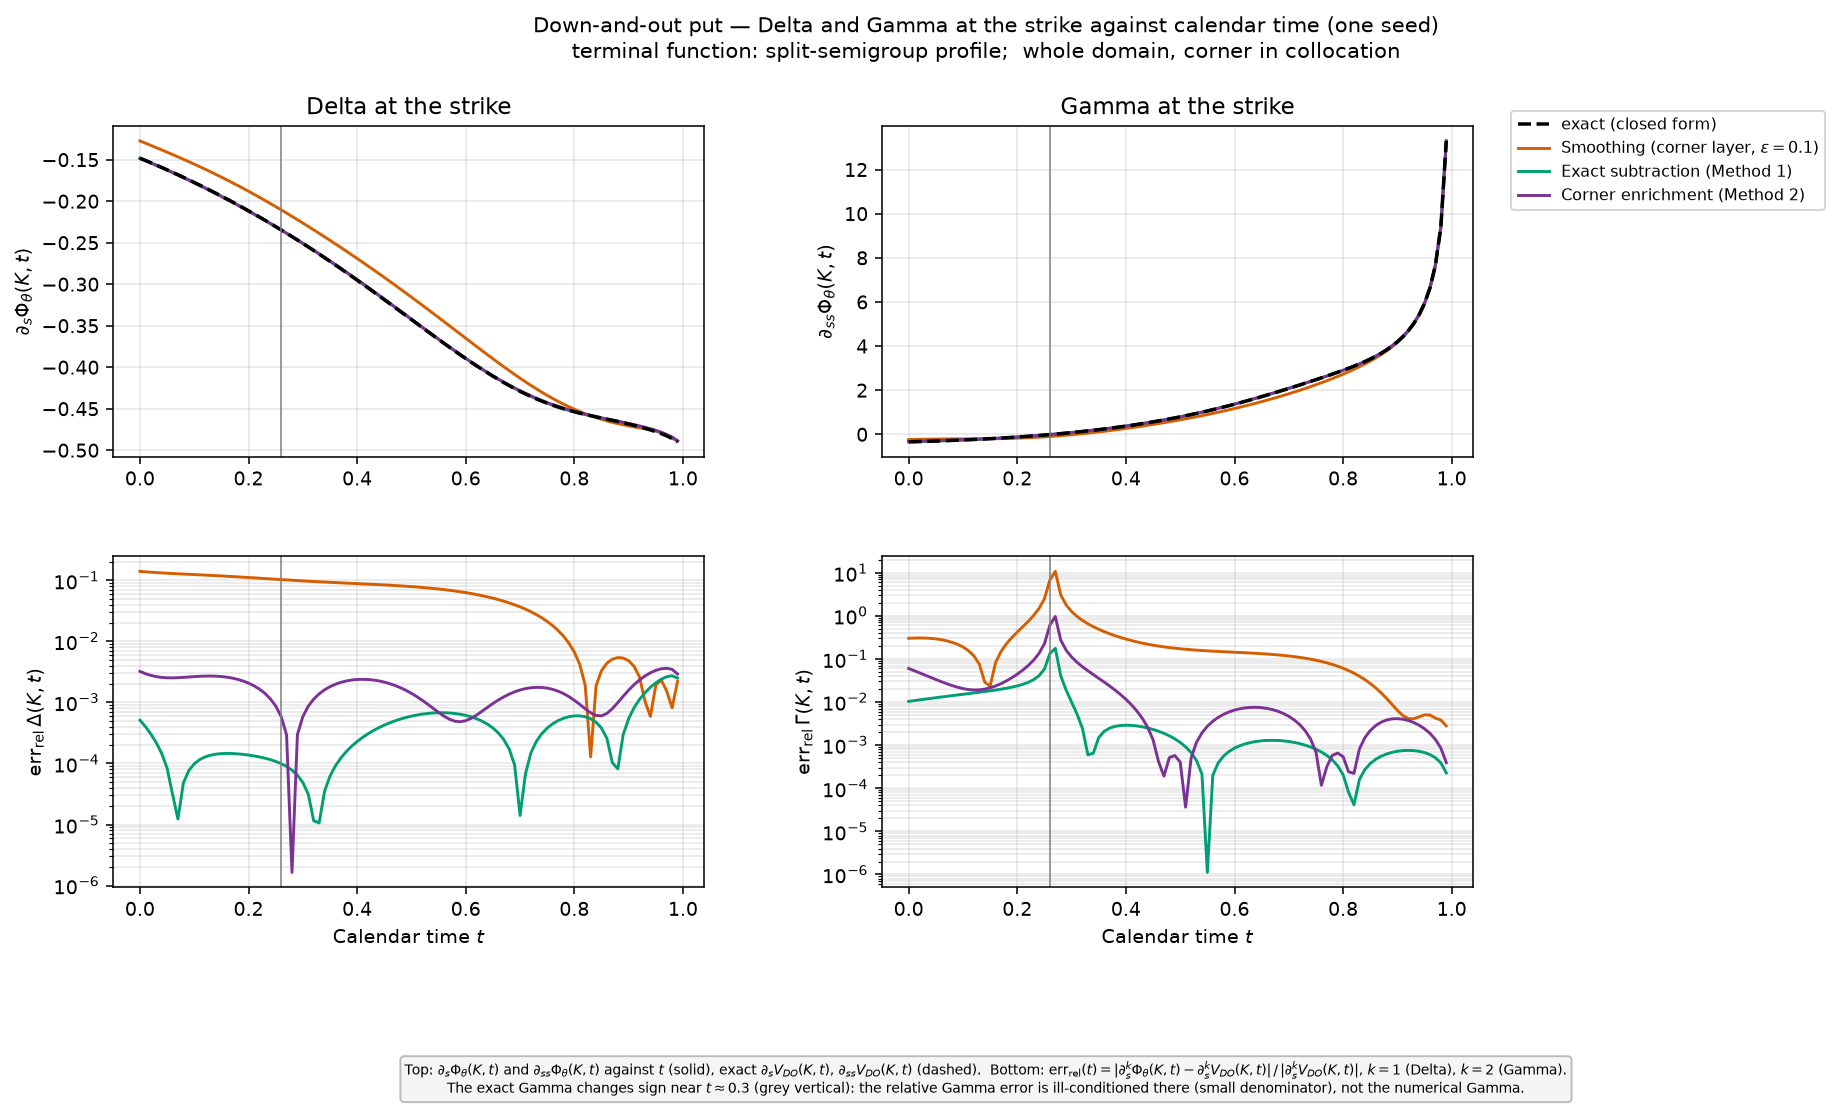
\includegraphics[width=0.95\linewidth]{figures/greeks_at_strike_vs_time_split.png}
\caption{Haut : $\partial_s\Phi_\theta(K,t)$ et $\partial_{ss}\Phi_\theta(K,t)$ en fonction de $t$ (traits pleins), valeurs exactes en tirets. Bas : $\mathrm{err}_{\mathrm{rel}}\,\Delta(t)$ et $\mathrm{err}_{\mathrm{rel}}\,\Gamma(t)$ (échelle log). La verticale grise marque le zéro de $\partial_{ss}V_{DO}(K,\cdot)$, où l'erreur relative est mal conditionnée.}
\label{fig:greeks-vs-t_split}
\end{figure}

\section{Ce qui sépare analytiquement l'enrichissement de la soustraction}
Les deux résolutions analytiques écrivent l'extension comme une partie singulière qui reproduit le saut du coin plus un reste régulier, $g_2 = S + h$ avec $\Delta = K-B$, et ne diffèrent que par le choix de $S$ : $S_{\mathrm{sub}} = \Delta\,V_{DOD}$ (la digitale down-and-out, Définition 7) contre $S_{\mathrm{enr}} = \chi(s)\,\Delta\,\mathrm{erf}(\xi)$ avec $\xi = \ln(s/B)/(\sigma\sqrt{2(T-t)})$ (le profil de similarité de la limite en temps court, Définition 8). Les deux reproduisent exactement les deux traces, donc les prix entraînés ne sont pas séparés par leurs contraintes : ce qui les sépare est le forçage intérieur que le réseau doit absorber. Ces figures sont des évaluations en forme fermée, en float64, sans aucun réseau entraîné. Source : \path{data/compare_singular_parts_subtraction_enrichment/20260924_blackscholes_d00.1_d10.3}.
\textbf{Mesuré sur la grille du domaine complet.} $\max|\mathcal L^{BS}S_{\mathrm{sub}}| = 0$ (exactement zéro en tout point, Proposition 4) contre $\max|\mathcal L^{BS}S_{\mathrm{enr}}| = 3.21$ et une moyenne quadratique de $0.392$ (Proposition 5 : de carré intégrable, non nul). La différence des deux parties singulières atteint $0.4$, soit $\Delta = K - B$ lui-même, tandis que celle des extensions complètes ne dépasse pas $0.0846$ : les parties régulières compensent l'essentiel de l'écart, et c'est bien le résidu, non la valeur de l'extension, qui sépare les deux méthodes.
\begin{landscape}
\begin{figure}[H]
\centering
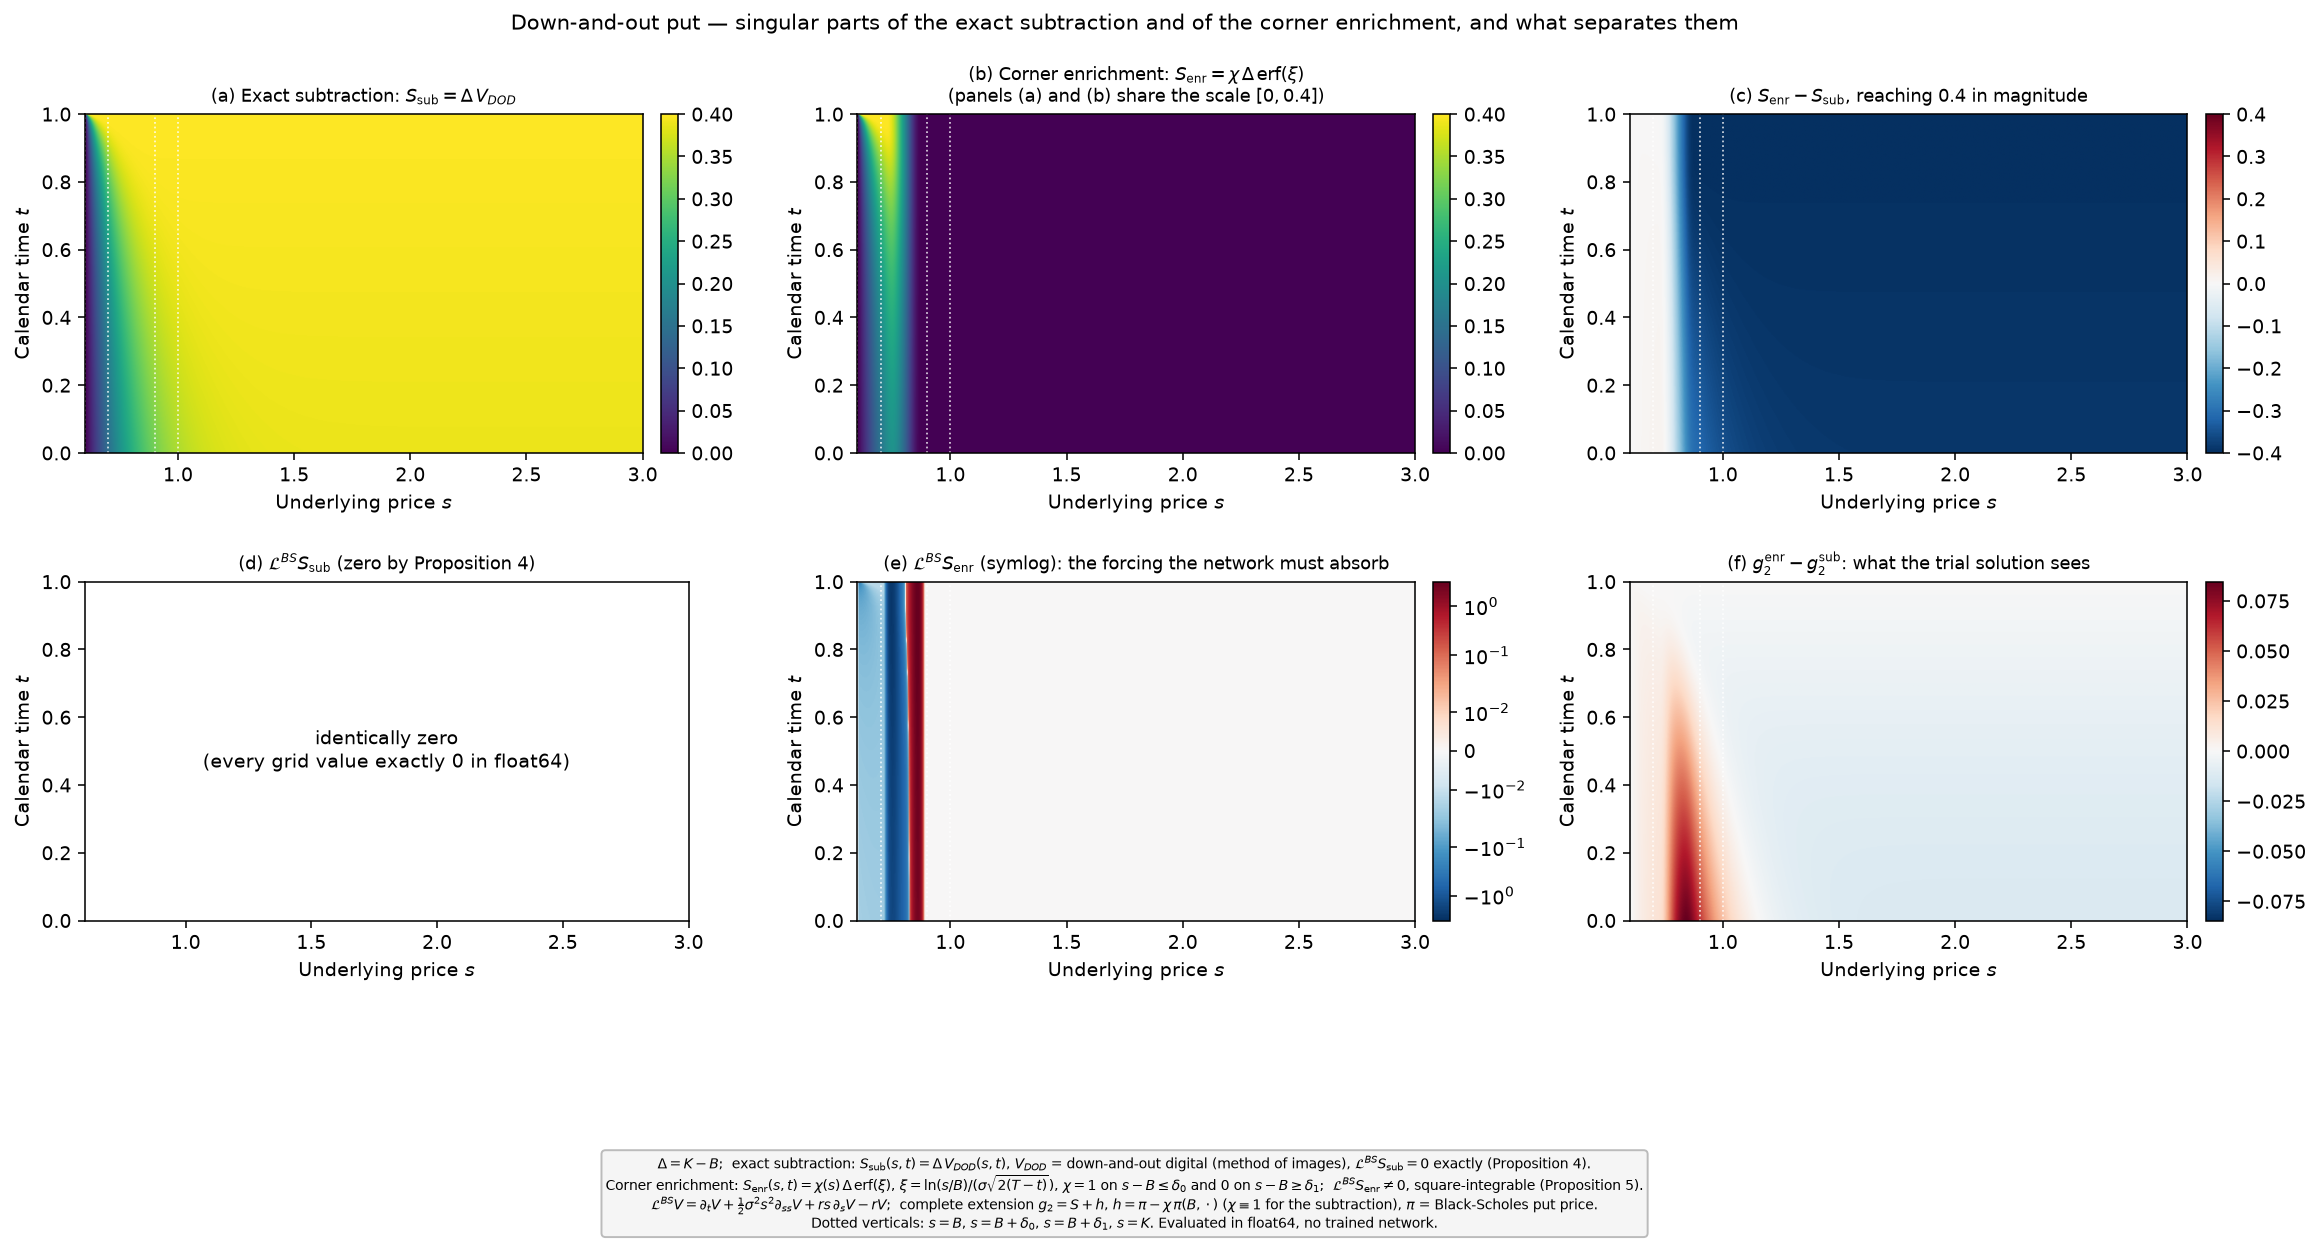
\includegraphics[width=\linewidth,height=0.8\textheight,keepaspectratio]{figures/singular_parts_and_difference.png}
\caption{(a) et (b) : les deux parties singulières sur la même échelle. La digitale $\Delta\,V_{DOD}$ monte de $0$ à la barrière jusqu'à $\Delta=0.4$ et le reste sur tout le domaine ; le profil de similarité, coupé par $\chi$, est nul au-delà de $s = B+\delta_1 = 0.9$. (c) : leur différence, qui vaut donc $-\Delta$ dans tout le champ lointain. (d) : $\mathcal L^{BS}S_{\mathrm{sub}}$, identiquement nul. (e) : $\mathcal L^{BS}S_{\mathrm{enr}}$ en échelle symlog, concentré dans la bande $[B, B+\delta_1]$ et d'amplitude d'ordre $1$ : c'est le forçage que le réseau doit absorber, et la raison pour laquelle la meilleure perte intérieure de l'enrichissement est un à deux ordres de grandeur au-dessus de celle de la soustraction. (f) : la différence des extensions complètes $g_2 = S + h$, plus petite d'un facteur $5$ que celle des parties singulières, les restes réguliers compensant la troncature de $\chi$.}
\label{fig:singular-parts}
\end{figure}

\end{landscape}

\begin{landscape}
\begin{figure}[H]
\centering
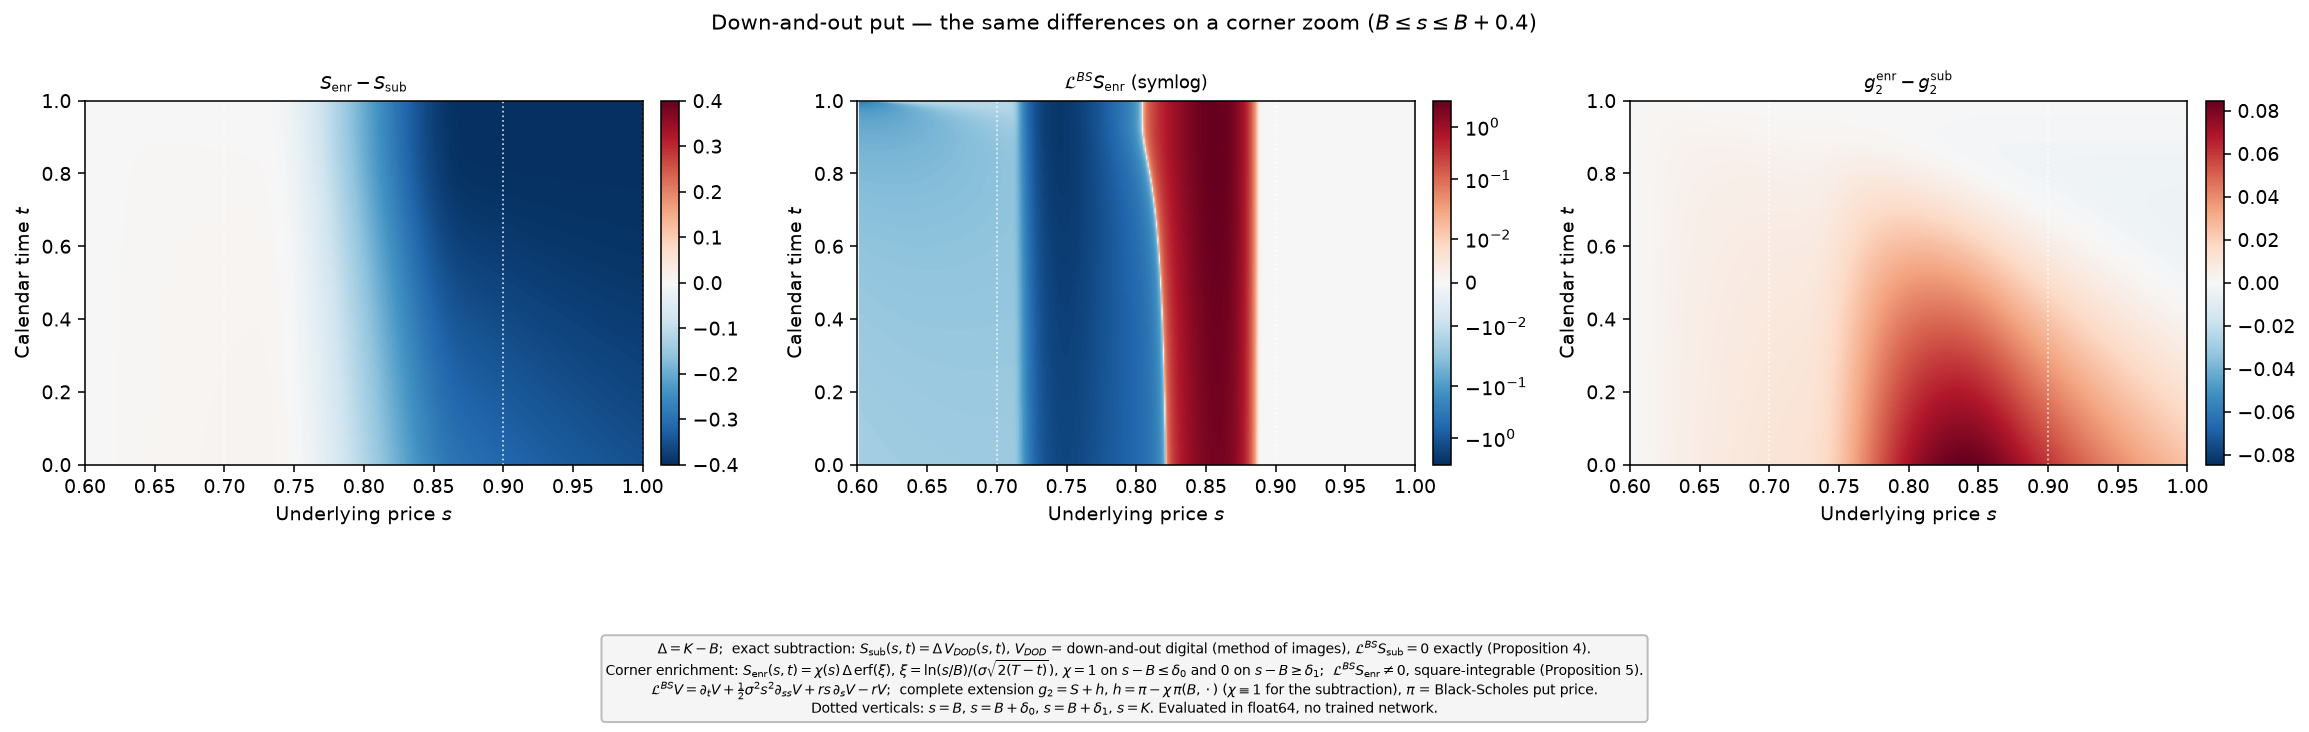
\includegraphics[width=\linewidth,height=0.8\textheight,keepaspectratio]{figures/singular_parts_corner_zoom.png}
\caption{Les mêmes différences sur un zoom du coin. Les verticales pointillées marquent $s=B$, $s=B+\delta_0$, $s=B+\delta_1$ et $s=K$.}
\label{fig:singular-parts-zoom}
\end{figure}

\end{landscape}

\begin{landscape}
\begin{figure}[H]
\centering
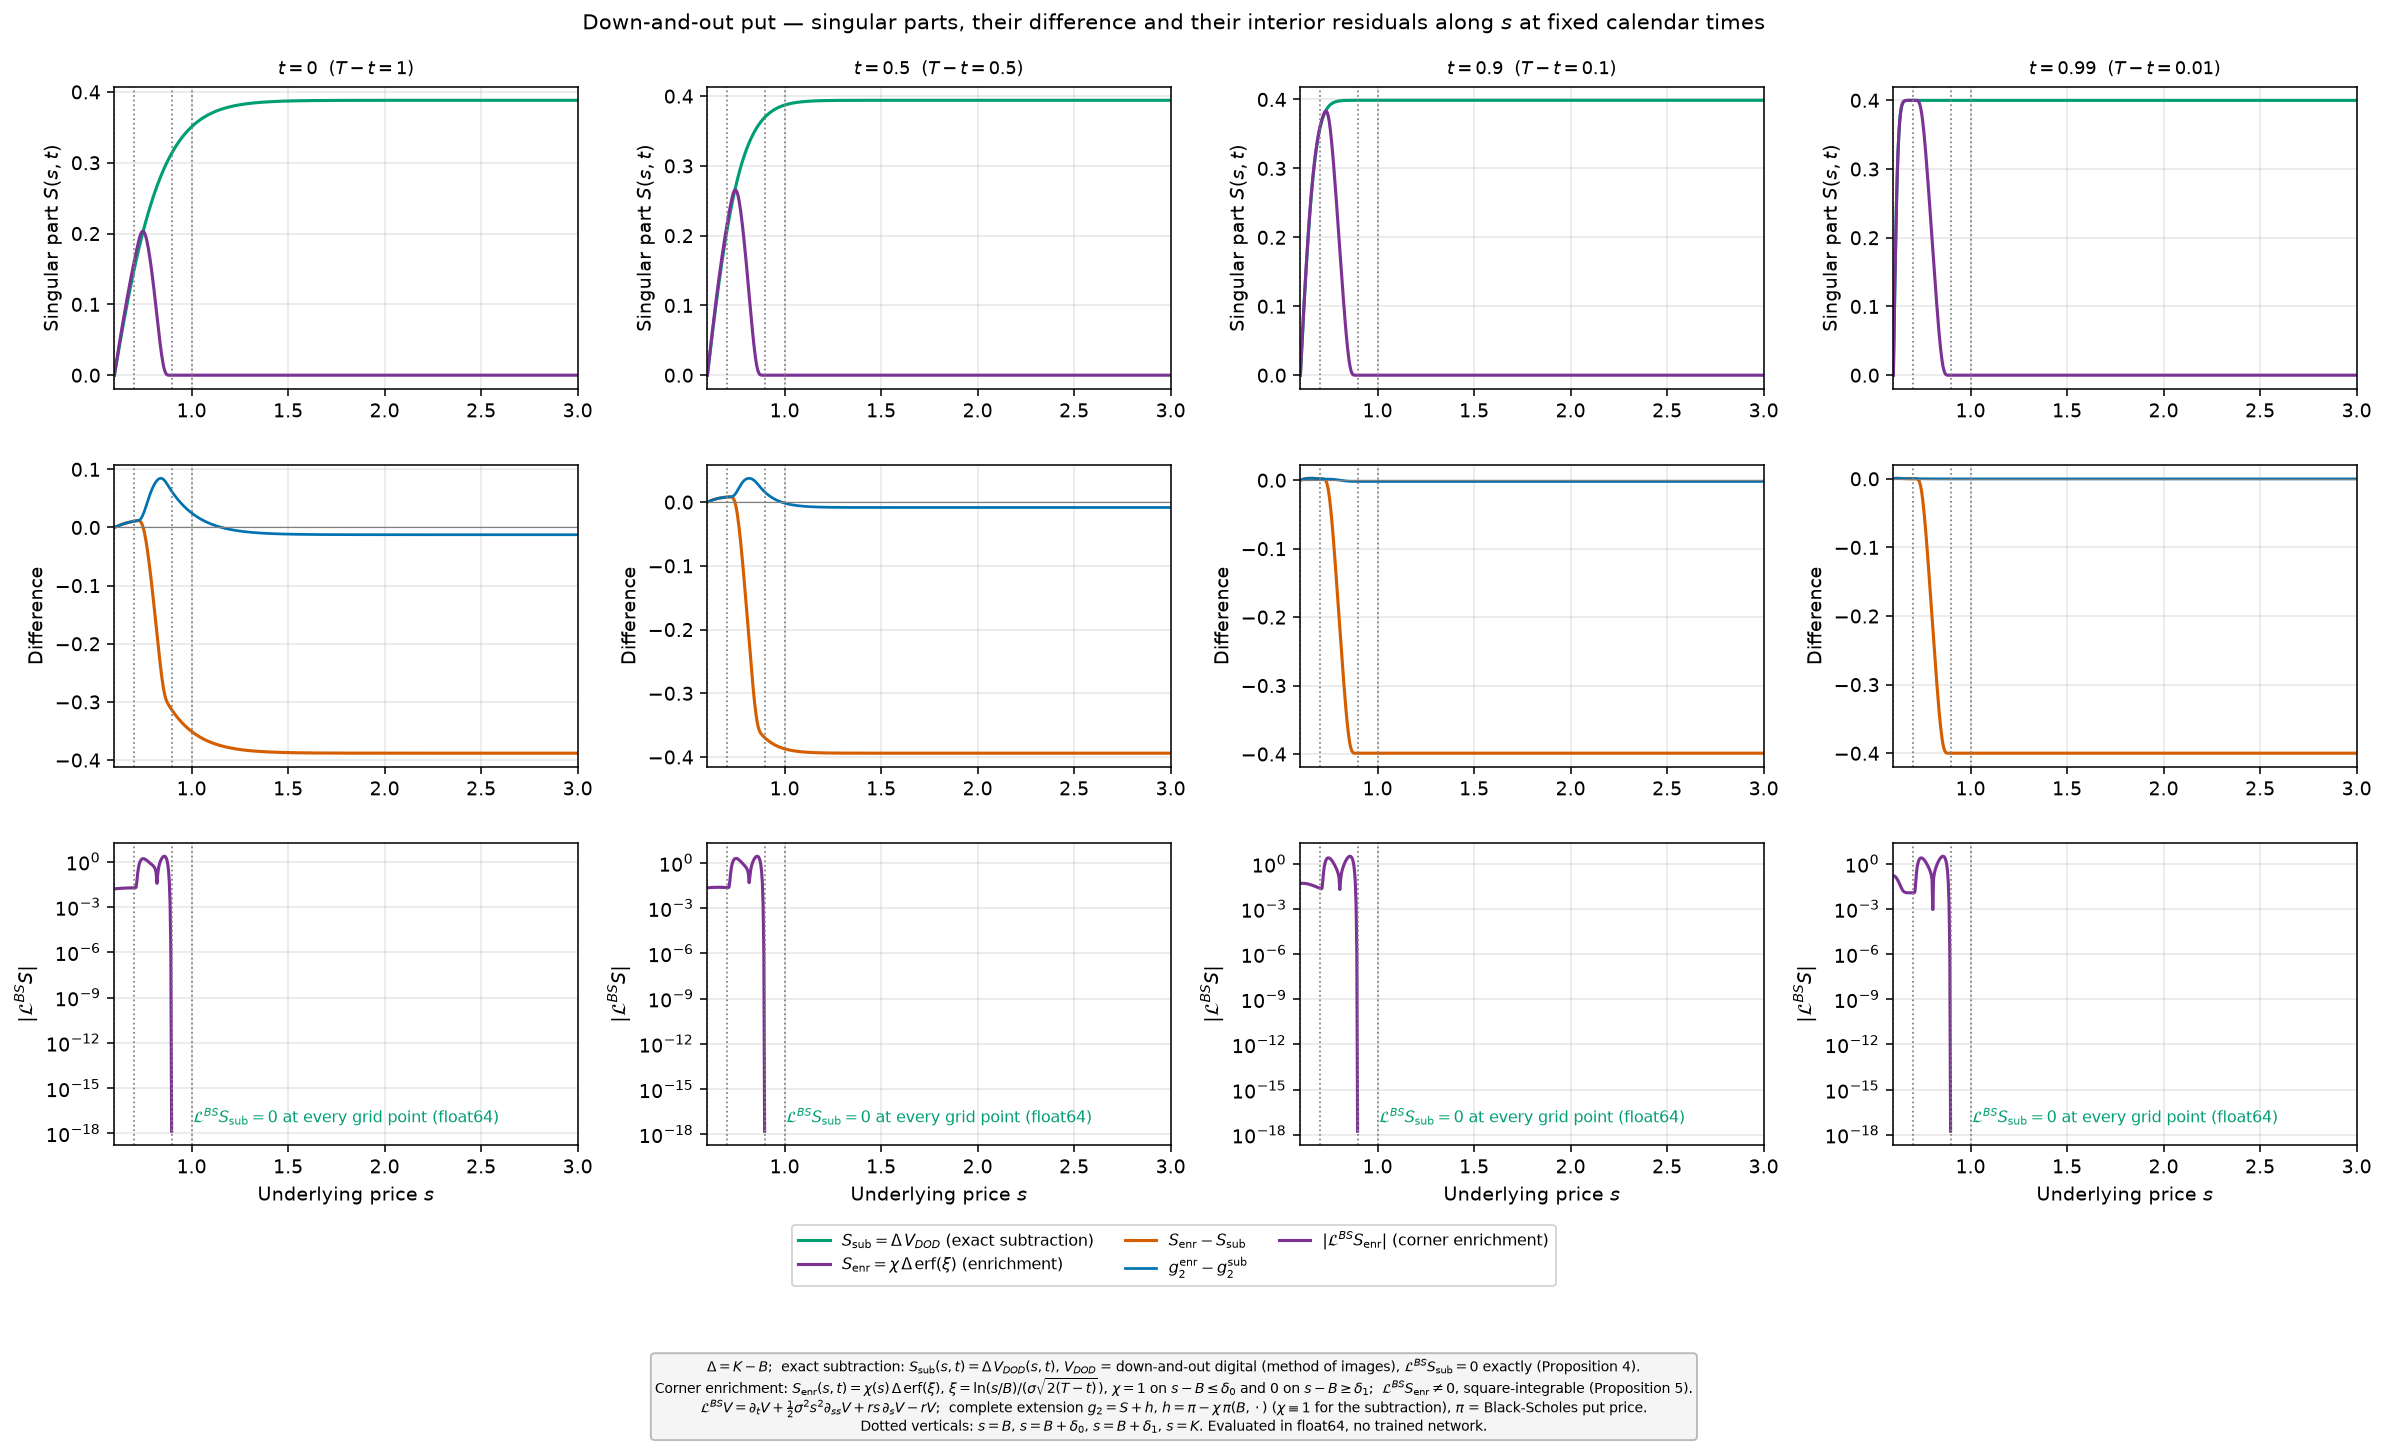
\includegraphics[width=\linewidth,height=0.8\textheight,keepaspectratio]{figures/singular_parts_slices.png}
\caption{Coupes en $s$ à $t$ fixé. Ligne du haut : les deux parties singulières ; la digitale (vert) croît de façon monotone vers $\Delta$, le profil de similarité (violet) culmine à $\Delta$ puis est ramené à zéro par le cutoff. Ligne du milieu : la différence des parties singulières (orange), qui sature à $-\Delta$, et celle des extensions complètes (bleu), qui reste sous $0.09$. Ligne du bas : $|\mathcal L^{BS}S|$ en échelle logarithmique ; celui de la soustraction est exactement nul et ne peut pas être tracé sur un axe logarithmique, ce que le panneau indique.}
\label{fig:singular-parts-slices}
\end{figure}

\end{landscape}

\section{Gamma de l'enrichissement contre Gamma de la soustraction}
La dérivée seconde en prix est la quantité la plus exposée au forçage intérieur de la section précédente, et c'est celle à réduire si l'enrichissement doit être amélioré. La figure de zoom du coin de la section précédente trace les deux traitements analytiques \emph{avec} le run de lissage, dont $\partial_{ss}\Phi_\theta$ oscille sur quatre décades dans le même panneau : à cette échelle les deux courbes analytiques sont confondues et leur écart n'est pas lisible. Les figures ci-dessous retirent le lissage et résolvent les deux traitements analytiques seuls, sur les cinq graines maîtresses. Évaluation ponctuelle en float64 à partir des modèles sauvegardés, sans réentraînement. Source : \path{data/compare_gamma_subtraction_enrichment/20260924_blackscholes_allseeds}.
\begin{table}[H]
\centering
\scriptsize
\begin{adjustbox}{max width=\textwidth}
\begin{tabular}{lcccc}
\toprule
\textbf{Bande $s-B$} & \textbf{Rôle du cutoff} & \textbf{$\|e_\Gamma\|_{L^2}$ soustraction} & \textbf{$\|e_\Gamma\|_{L^2}$ enrichissement} & \textbf{Rapport} \\
\midrule
$[0, 0.1)$ & plateau, $\chi\equiv1$ & 2.384e-02 & 8.113e-02 & 3.4 \\
$[0.1, 0.3)$ & transition, $\chi'\neq0$ & 7.270e-04 & 2.566e-02 & 35.3 \\
$[0.3, 0.4)$ & $\chi\equiv0$, avant le strike & 2.598e-04 & 4.196e-03 & 16.2 \\
$[0.4, 0.6)$ & $\chi\equiv0$, après le strike & 1.999e-04 & 1.401e-03 & 7.0 \\
\bottomrule
\end{tabular}
\end{adjustbox}
\caption{Norme $L^2$ en $s$ de l'erreur de Gamma sur chaque bande de prix, médiane sur les cinq graines puis moyenne sur le temps calendaire. Le rapport est le facteur que l'enrichissement doit gagner pour rejoindre la soustraction.}
\label{tab:gamma-bands}
\end{table}

\begin{landscape}
\begin{figure}[H]
\centering
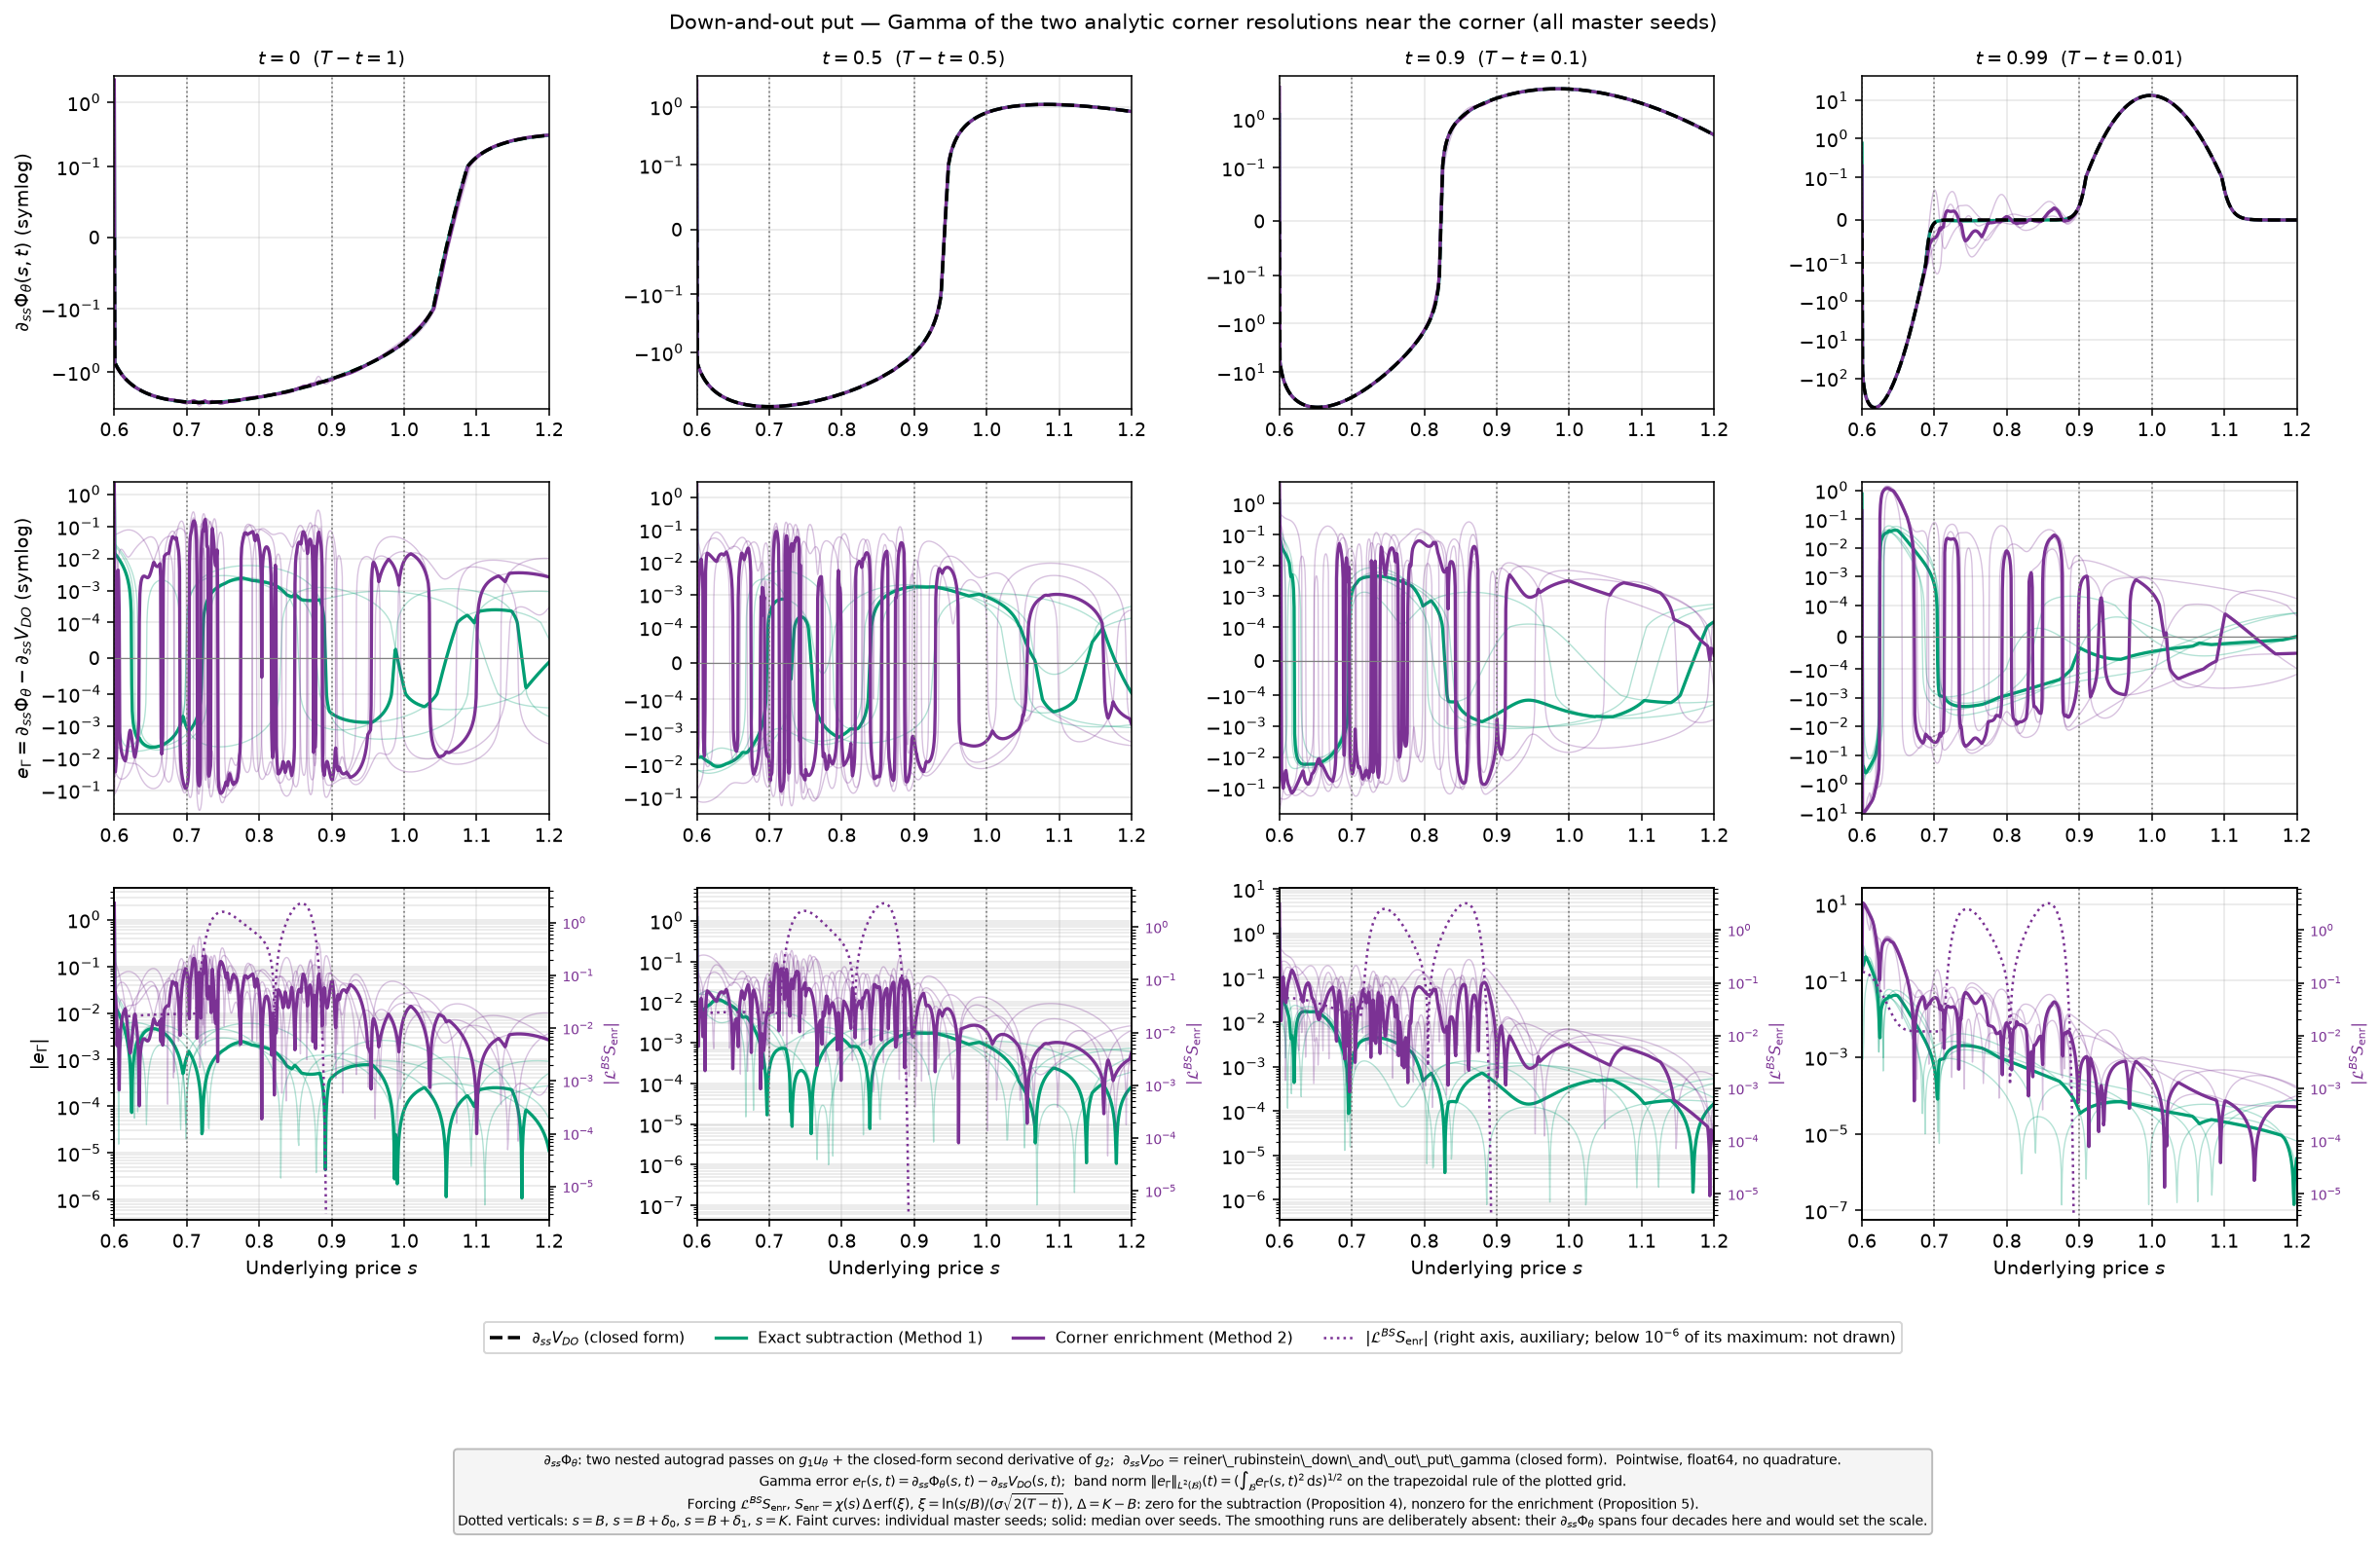
\includegraphics[width=\linewidth,height=0.8\textheight,keepaspectratio]{figures/gamma_profiles_corner.png}
\caption{Ligne du haut : $\partial_{ss}\Phi_\theta(s,t)$ des deux traitements (médiane sur les graines en trait épais, graines individuelles en trait fin) et $\partial_{ss}V_{DO}$ en tirets noirs. Ligne du milieu : l'erreur signée $e_\Gamma$, en échelle symlog. Ligne du bas : $|e_\Gamma|$ en échelle logarithmique, avec $|\mathcal L^{BS}S_{\mathrm{enr}}|$ superposé en pointillé sur l'axe de droite. La lecture : l'erreur de Gamma de l'enrichissement oscille entre la barrière et $s=B+\delta_1=0.9$, exactement le support du forçage, et rejoint celle de la soustraction au-delà.}
\label{fig:gamma-profiles}
\end{figure}

\end{landscape}

\begin{landscape}
\begin{figure}[H]
\centering
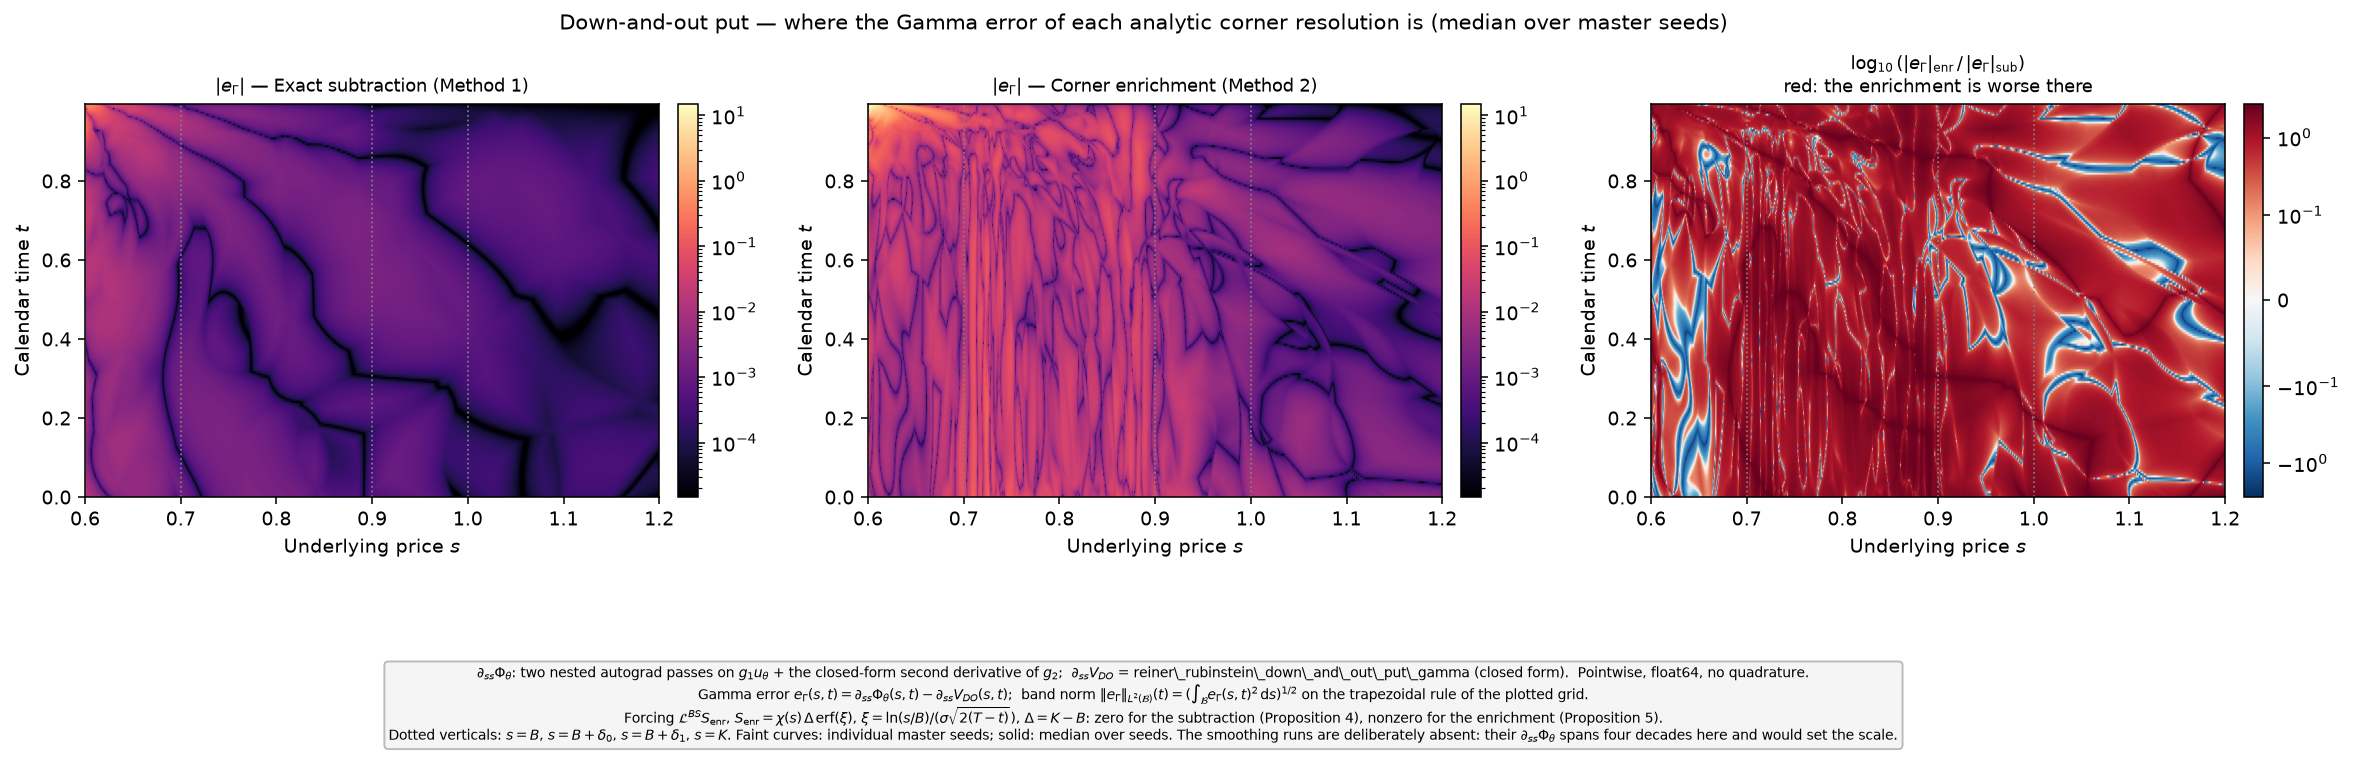
\includegraphics[width=\linewidth,height=0.8\textheight,keepaspectratio]{figures/gamma_error_heatmaps.png}
\caption{$|e_\Gamma|$ sur $(s,t)$ pour chaque traitement, échelle logarithmique commune, médiane sur les graines ; à droite leur rapport en $\log_{10}$. Le rouge domine : l'enrichissement est moins bon presque partout. Les filaments bleus sont les lignes nodales où l'erreur de l'un des deux change de signe et passe par zéro, pas des régions où l'enrichissement est meilleur. La tranche terminale $t=T$ est exclue : l'erreur y est nulle par construction.}
\label{fig:gamma-heatmaps}
\end{figure}

\end{landscape}

\begin{landscape}
\begin{figure}[H]
\centering
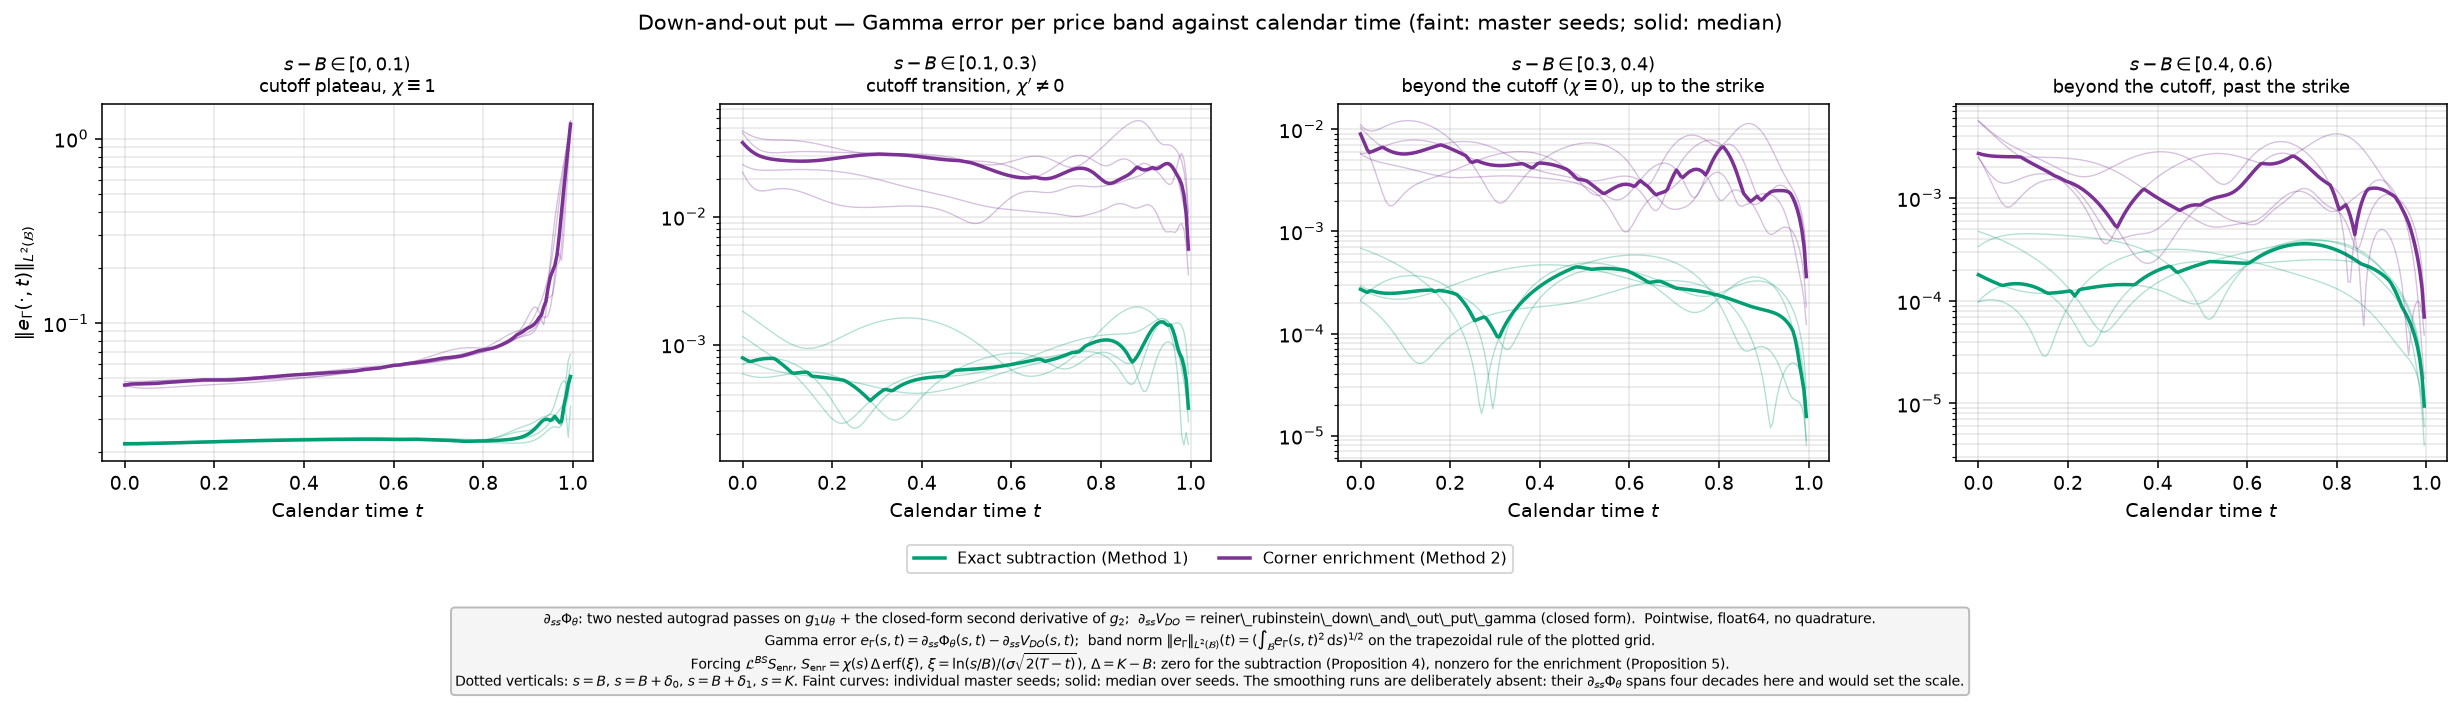
\includegraphics[width=\linewidth,height=0.8\textheight,keepaspectratio]{figures/gamma_error_by_band.png}
\caption{Norme $L^2$ en $s$ de l'erreur de Gamma sur chaque bande, en fonction du temps calendaire ; traits fins : graines individuelles. L'écart entre les deux traitements est reproductible sur les cinq graines (les faisceaux ne se croisent pas dans les deux premières bandes), donc il vient de la construction et non du bruit d'optimisation.}
\label{fig:gamma-bands}
\end{figure}

\end{landscape}

\section{Figures par run (graine 0)}
Pour chaque configuration, le run de la graine 0 : surface de prix sur la grille d'évaluation (entraîné, forme fermée, différence signée) ; coupes $V(s,t)$ à $t$ fixé en échelle symlog (linéaire sous $10^{-6}$, logarithmique au-delà) --- le prix va de $0.4$ près de la barrière à $10^{-5}$ dans le champ lointain, invisible en linéaire, et un prix entraîné qui change de signe y apparaît comme un passage sous zéro, pas comme une chute vers un plancher ; et, pour les traitements analytiques, la décomposition de l'estimateur $\Phi_\theta=S+h+g_1u_\theta$ ($S=\Delta V_{DOD}$ ou $S=\chi\Delta\,\mathrm{erf}(\xi)$, $h=\pi-\chi\,\pi(B,\cdot)$). Cette dernière montre ce que la partie en forme fermée reproduit à elle seule, ce que l'extension régulière ajoute et ce qui reste au réseau : pour la soustraction le réseau est presque nul (l'ansatz porte la solution) ; pour l'enrichissement $E$ est localisé par $\chi$ et $h$ présente un creux compensateur dans la bande de transition $[B+\delta_0,B+\delta_1]$, que le réseau doit corriger --- c'est là que se situe son surcroît d'erreur.
\subsection{Raw payoff $(K-s)^+$ [whole domain: corner in collocation]}
. Run : \path{20260923_113930_iters50000_eps0.1_seed0}.
\begin{figure}[H]
\centering
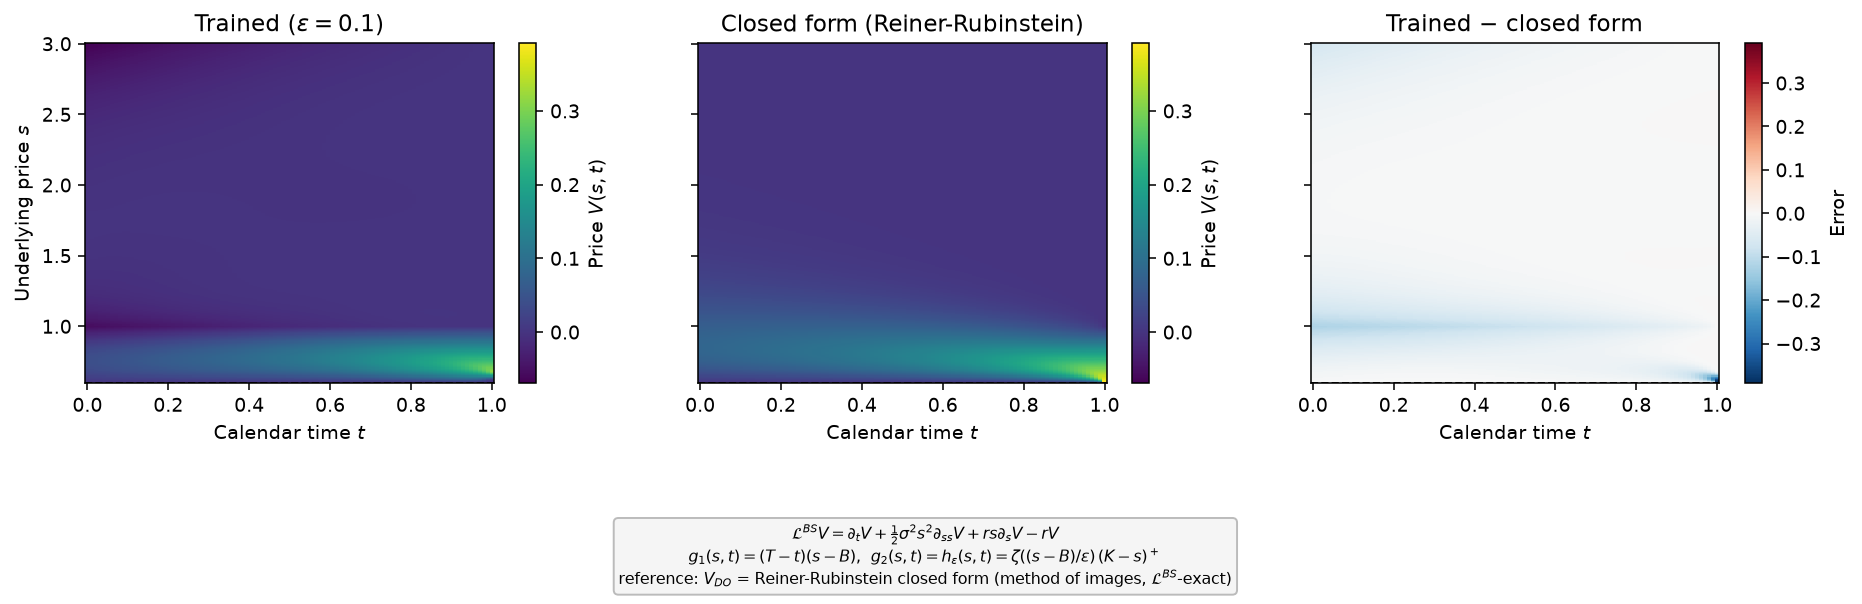
\includegraphics[width=\linewidth]{figures/raw_corner_included_seed0_price_surface_eps0.1.png}
\caption{Surface de prix : solution entraînée, forme fermée, différence. .}
\label{fig:raw_corner_included-price_surface_eps0.1}
\end{figure}

\begin{figure}[H]
\centering
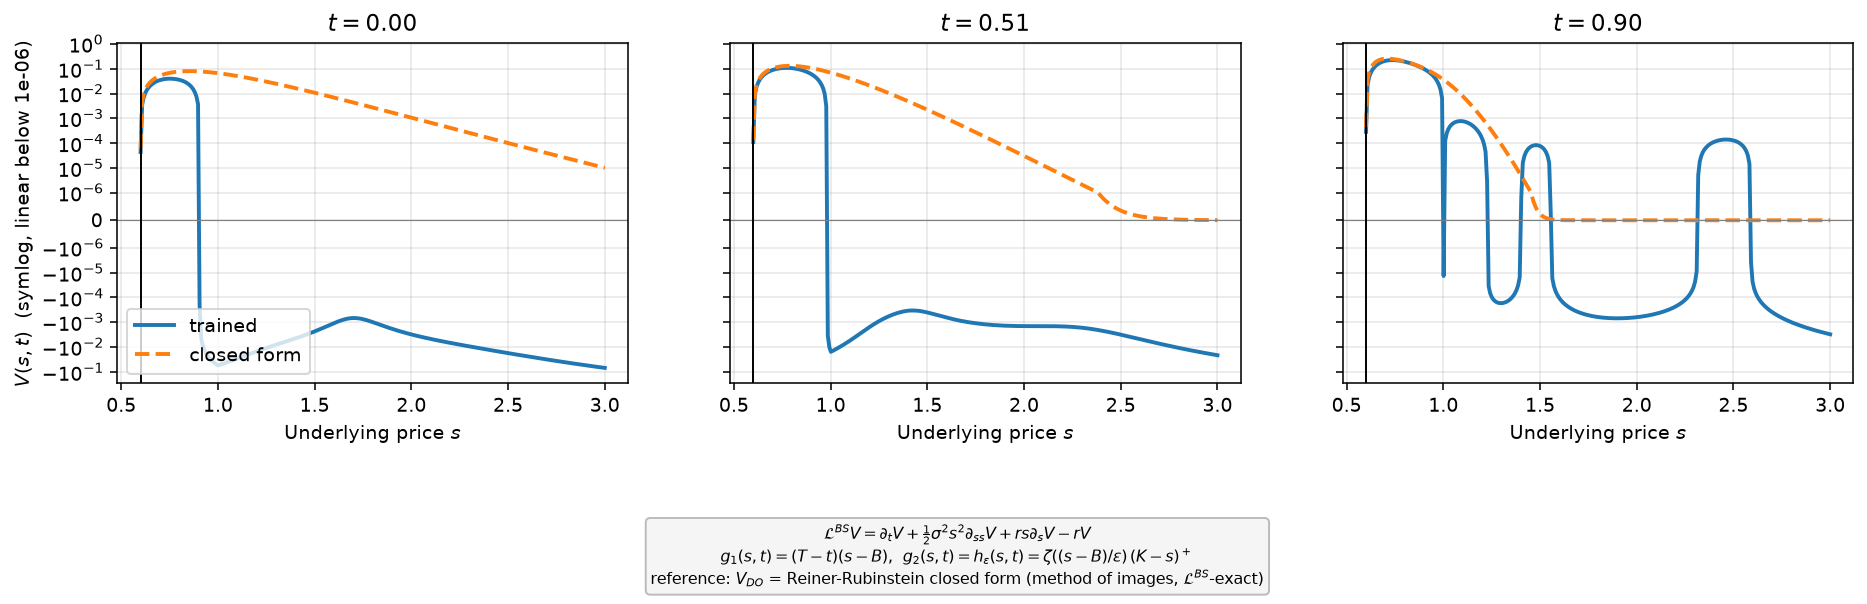
\includegraphics[width=\linewidth]{figures/raw_corner_included_seed0_log_slice_eps0.1.png}
\caption{Coupes $V(s,t)$ à $t\in\{0,0.5,0.9\}$, échelle symlog (solution entraînée en trait plein, forme fermée en tirets ; trait vertical : $s=B$). .}
\label{fig:raw_corner_included-log_slice_eps0.1}
\end{figure}

\subsection{Black-Scholes put price (ordinary autograd route) [whole domain: corner in collocation]}
. Run : \path{20260923_113717_iters50000_eps0.1_seed0_blackscholes}.
\begin{figure}[H]
\centering
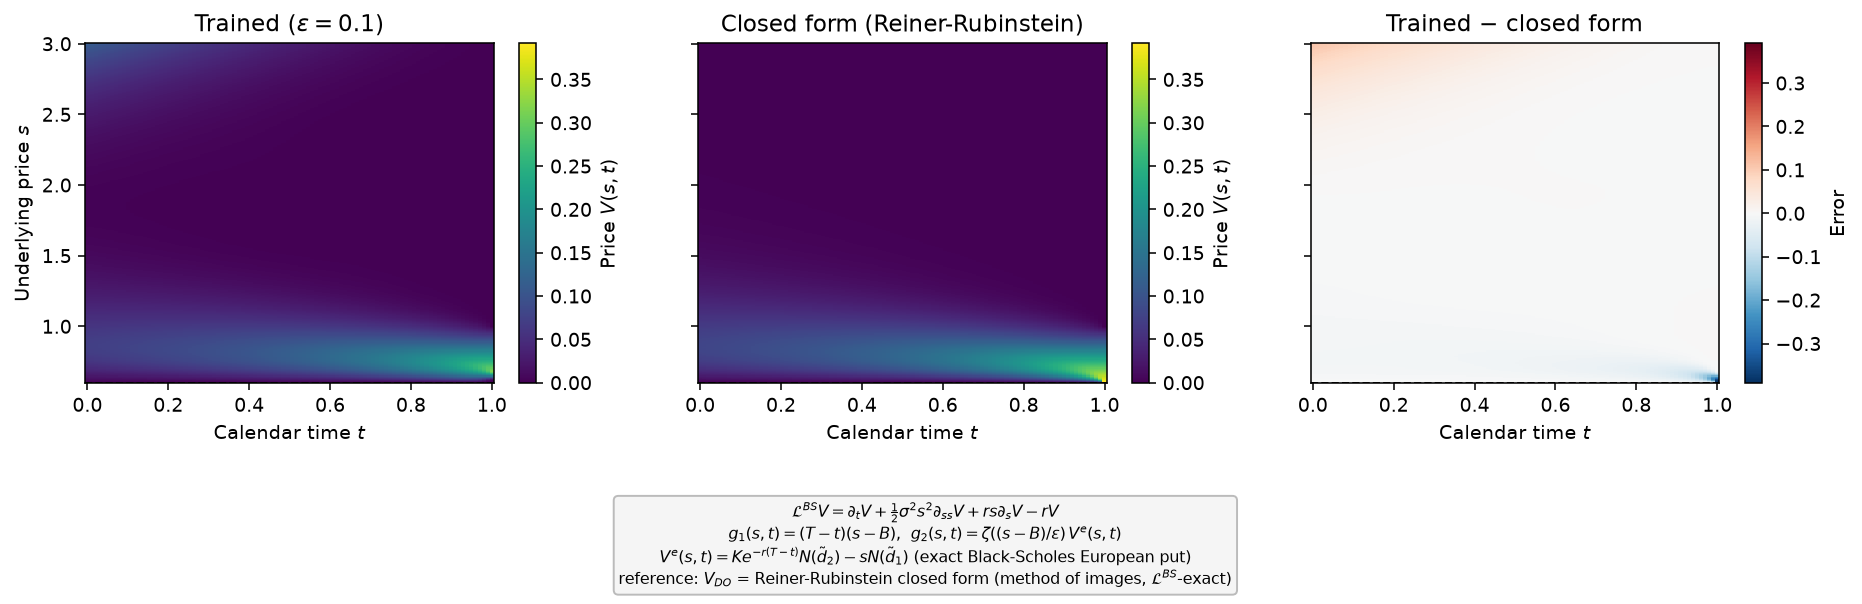
\includegraphics[width=\linewidth]{figures/blackscholes_corner_included_seed0_price_surface_eps0.1.png}
\caption{Surface de prix : solution entraînée, forme fermée, différence. .}
\label{fig:blackscholes_corner_included-price_surface_eps0.1}
\end{figure}

\begin{figure}[H]
\centering
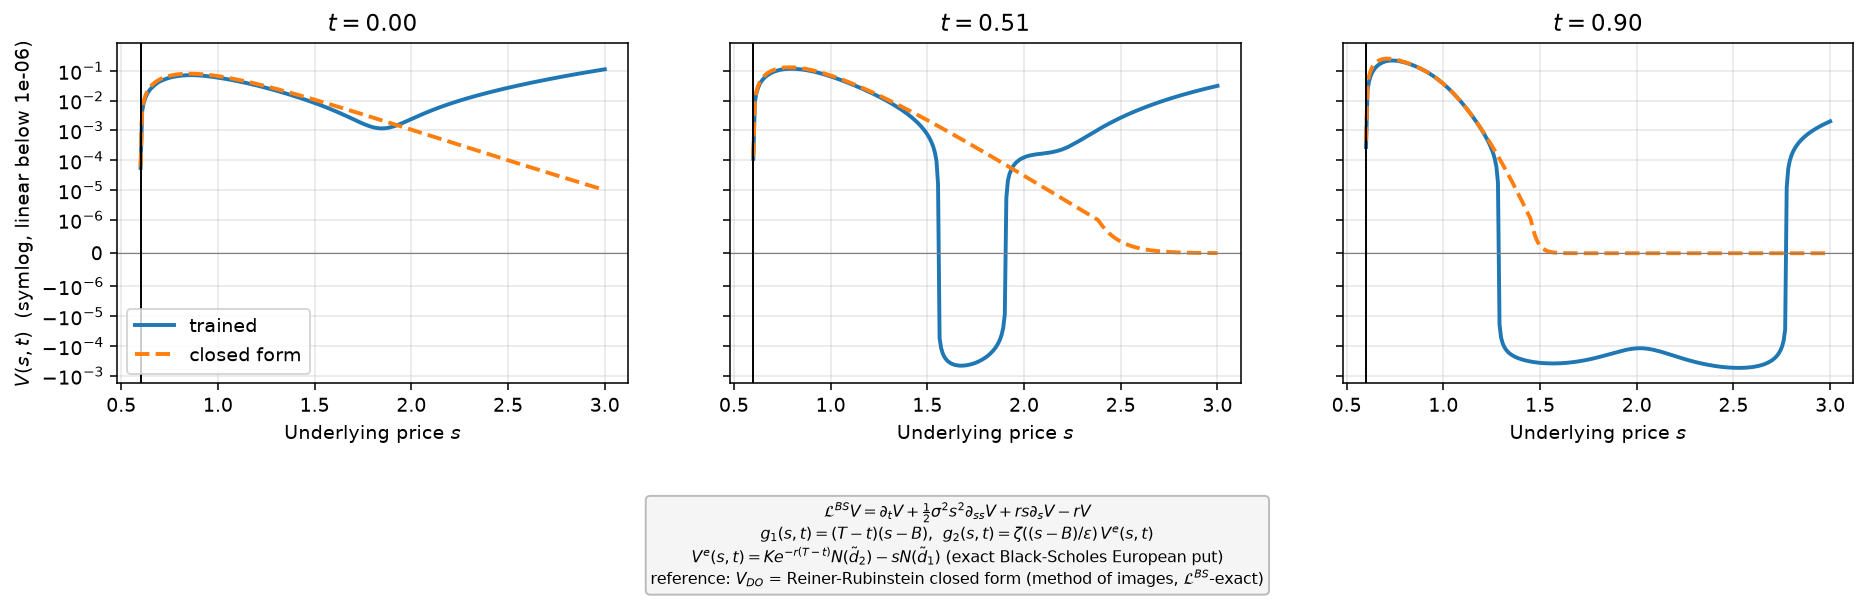
\includegraphics[width=\linewidth]{figures/blackscholes_corner_included_seed0_log_slice_eps0.1.png}
\caption{Coupes $V(s,t)$ à $t\in\{0,0.5,0.9\}$, échelle symlog (solution entraînée en trait plein, forme fermée en tirets ; trait vertical : $s=B$). .}
\label{fig:blackscholes_corner_included-log_slice_eps0.1}
\end{figure}

\subsection{Black-Scholes put price (two-term analytic-residual route) [whole domain: corner in collocation]}
. Run : \path{20260923_123231_iters50000_eps0.1_seed0_blackscholes_analyticres}.
\begin{figure}[H]
\centering
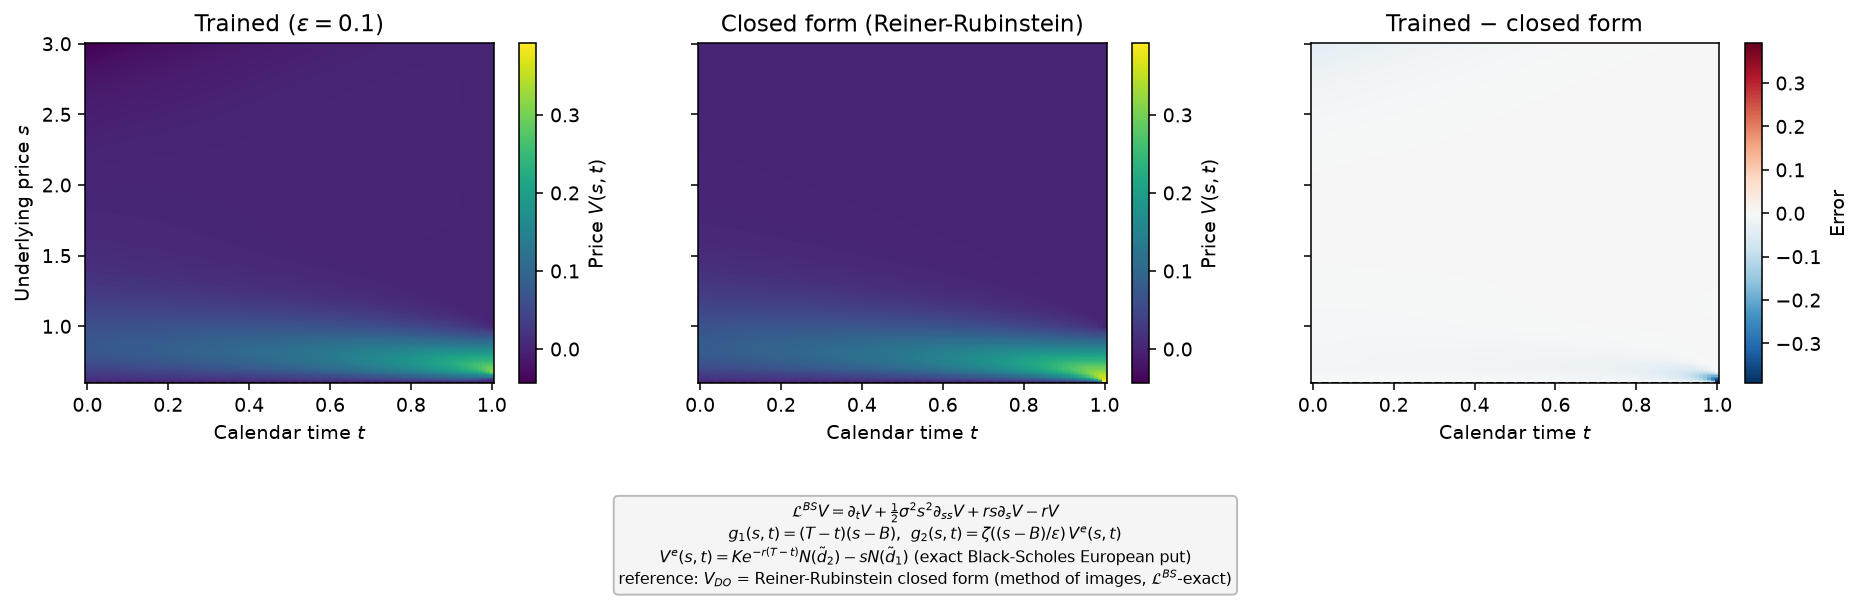
\includegraphics[width=\linewidth]{figures/blackscholes_analyticres_corner_included_seed0_price_surface_eps0.1.png}
\caption{Surface de prix : solution entraînée, forme fermée, différence. .}
\label{fig:blackscholes_analyticres_corner_included-price_surface_eps0.1}
\end{figure}

\begin{figure}[H]
\centering
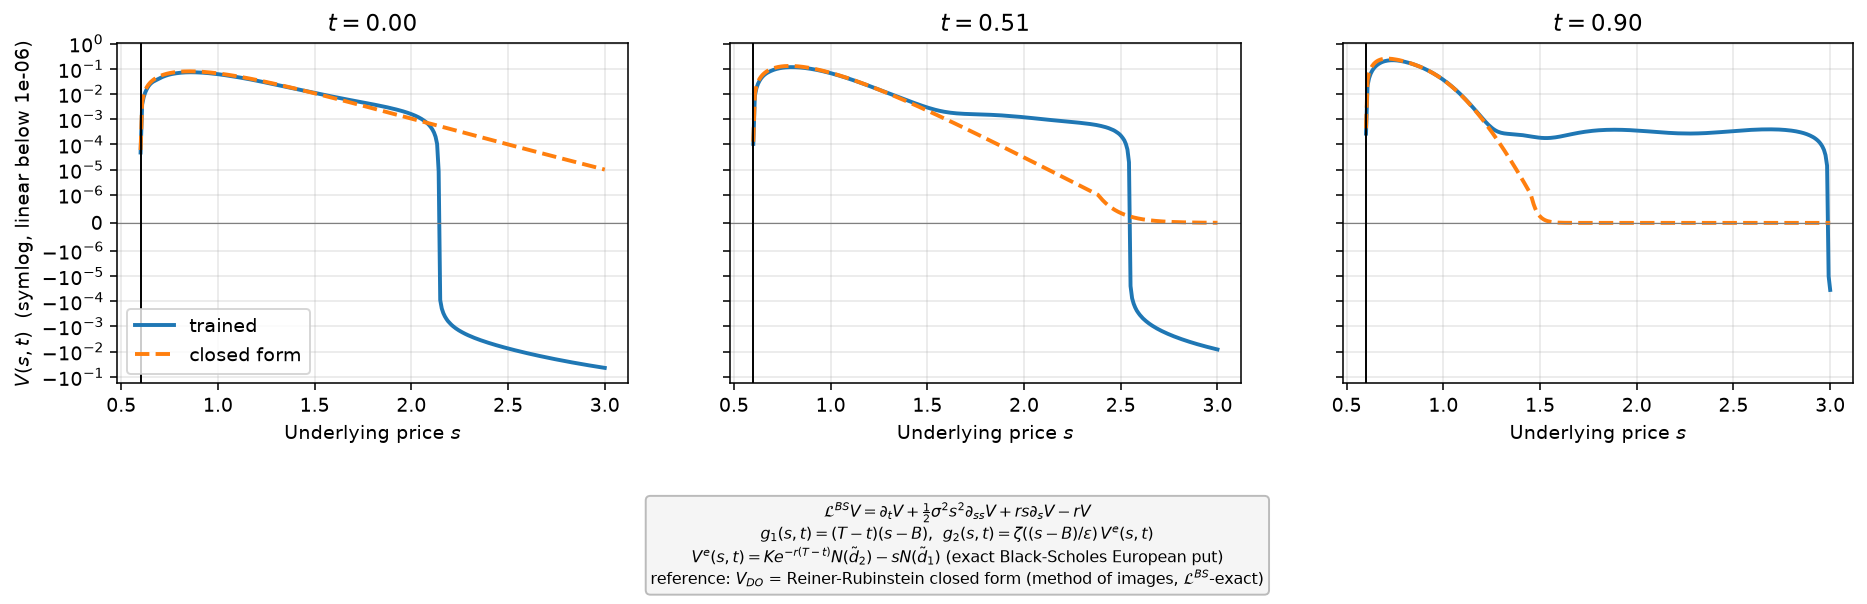
\includegraphics[width=\linewidth]{figures/blackscholes_analyticres_corner_included_seed0_log_slice_eps0.1.png}
\caption{Coupes $V(s,t)$ à $t\in\{0,0.5,0.9\}$, échelle symlog (solution entraînée en trait plein, forme fermée en tirets ; trait vertical : $s=B$). .}
\label{fig:blackscholes_analyticres_corner_included-log_slice_eps0.1}
\end{figure}

\subsection{Split-semigroup profile [whole domain: corner in collocation]}
. Run : \path{20260923_132013_iters50000_eps0.1_seed0_split_nuc0.3_closedform}.
\begin{figure}[H]
\centering
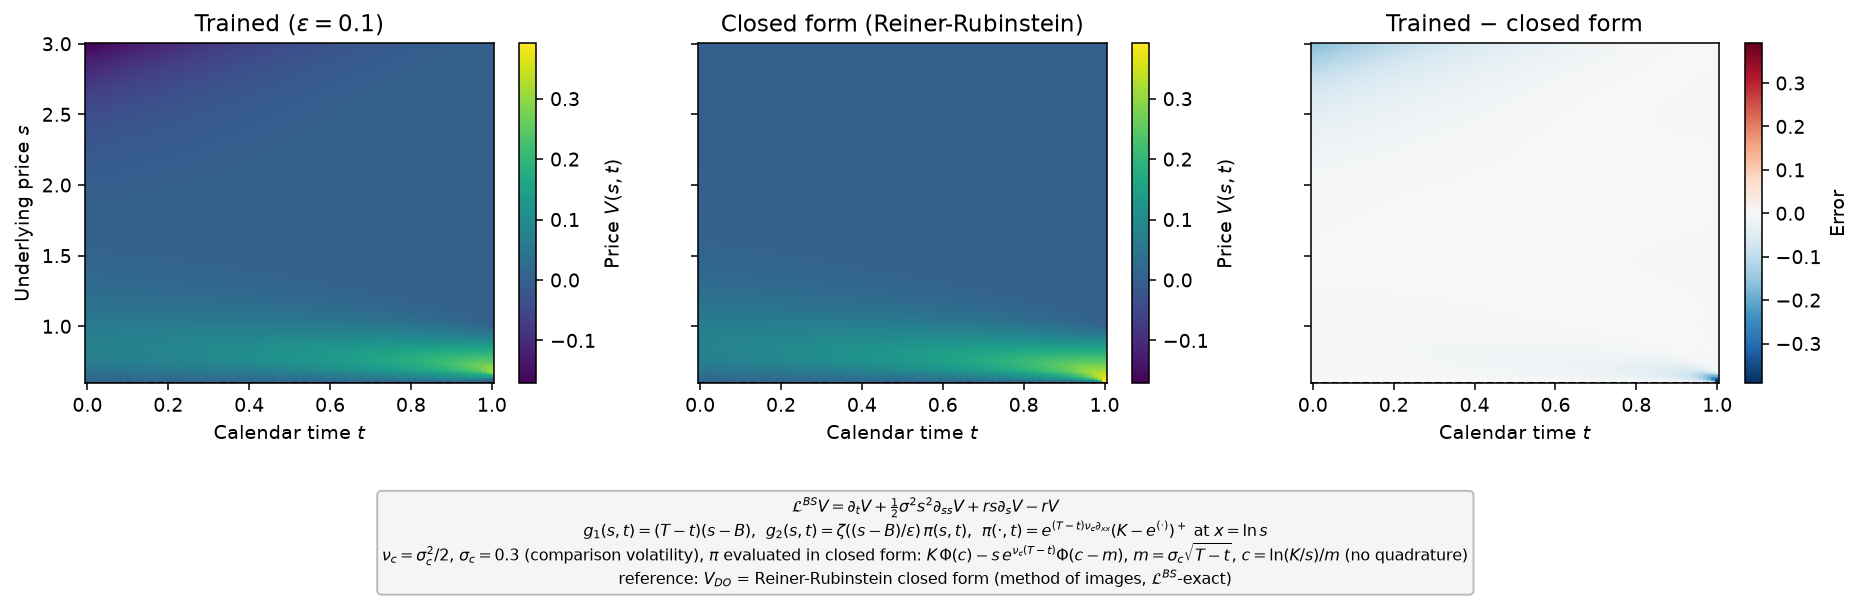
\includegraphics[width=\linewidth]{figures/split_corner_included_seed0_price_surface_eps0.1.png}
\caption{Surface de prix : solution entraînée, forme fermée, différence. .}
\label{fig:split_corner_included-price_surface_eps0.1}
\end{figure}

\begin{figure}[H]
\centering
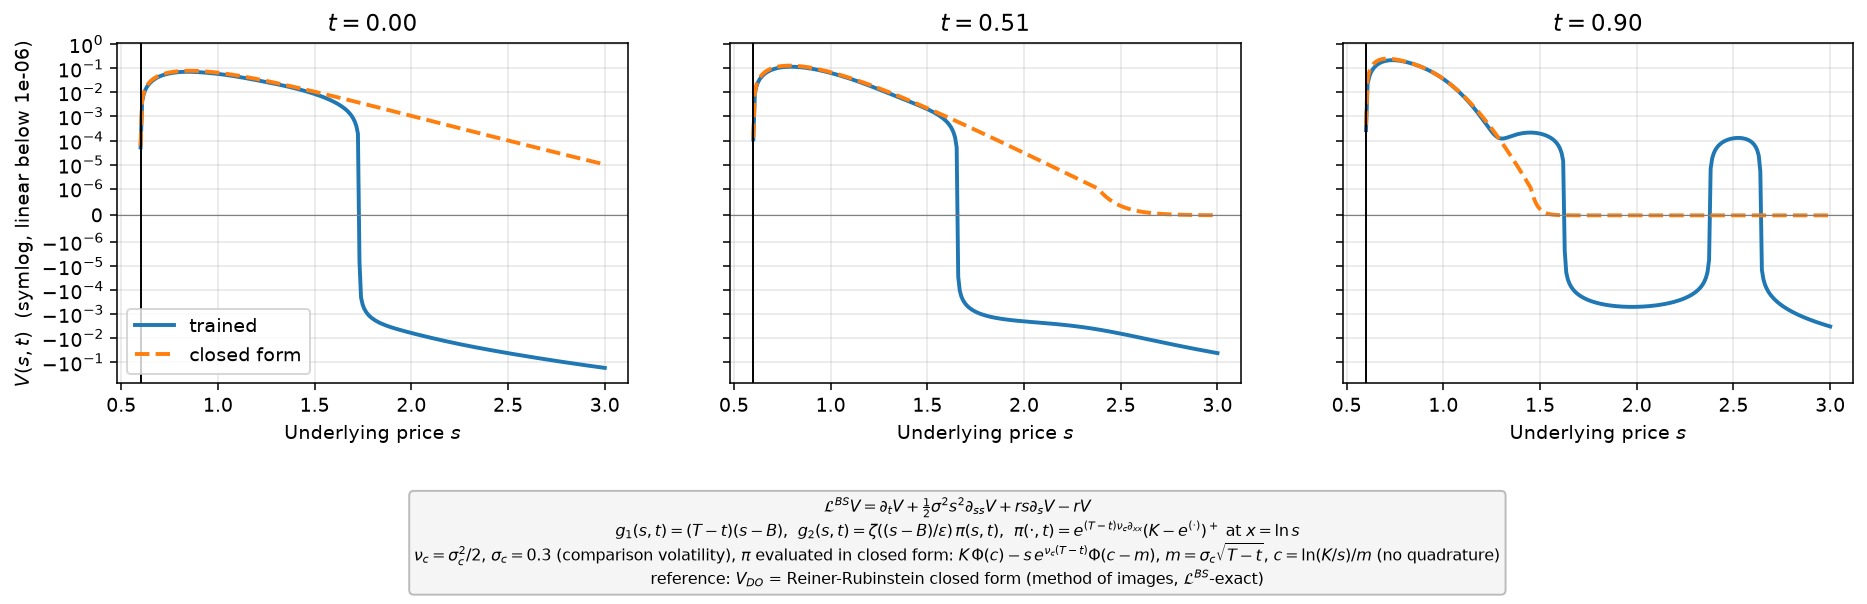
\includegraphics[width=\linewidth]{figures/split_corner_included_seed0_log_slice_eps0.1.png}
\caption{Coupes $V(s,t)$ à $t\in\{0,0.5,0.9\}$, échelle symlog (solution entraînée en trait plein, forme fermée en tirets ; trait vertical : $s=B$). .}
\label{fig:split_corner_included-log_slice_eps0.1}
\end{figure}

\subsection{Exact subtraction, raw payoff profile}
soustraction exacte ($\Delta V_{DOD}$), profil payoff brut (contrôle négatif). Run : \path{20260920_201745_iters50000_eps0_seed0_subtraction_raw}.
\begin{figure}[H]
\centering
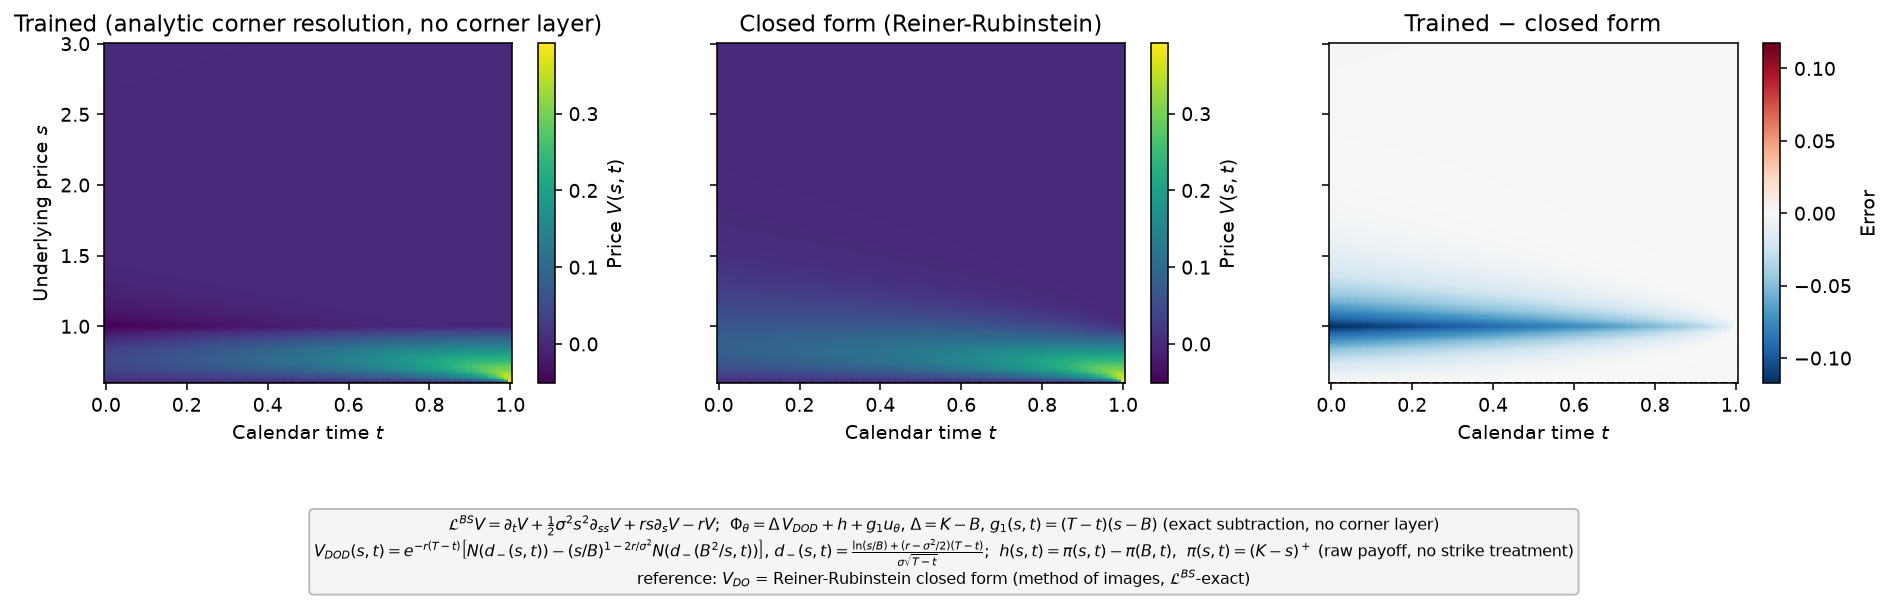
\includegraphics[width=\linewidth]{figures/subtraction_raw_seed0_price_surface_eps0.png}
\caption{Surface de prix : solution entraînée, forme fermée, différence. soustraction exacte ($\Delta V_{DOD}$), profil payoff brut (contrôle négatif).}
\label{fig:subtraction_raw-price_surface_eps0}
\end{figure}

\begin{figure}[H]
\centering

\includegraphics[width=\linewidth]{figures/subtraction_raw_seed0_log_slice_eps0.png}
\caption{Coupes $V(s,t)$ à $t\in\{0,0.5,0.9\}$, échelle symlog (solution entraînée en trait plein, forme fermée en tirets ; trait vertical : $s=B$). soustraction exacte ($\Delta V_{DOD}$), profil payoff brut (contrôle négatif).}
\label{fig:subtraction_raw-log_slice_eps0}
\end{figure}

\begin{figure}[H]
\centering

\includegraphics[width=\linewidth]{figures/subtraction_raw_seed0_subtraction_decomposition.png}
\caption{Décomposition de l'estimateur : partie singulière en forme fermée, extension régulière $h$, réseau $g_1u_\theta$, total, contre $V_{DO}$. soustraction exacte ($\Delta V_{DOD}$), profil payoff brut (contrôle négatif).}
\label{fig:subtraction_raw-subtraction_decomposition}
\end{figure}

\subsection{Exact subtraction, Black-Scholes profile}
soustraction exacte ($\Delta V_{DOD}$), profil Black--Scholes $V^e$. Run : \path{20260920_201746_iters50000_eps0_seed0_subtraction_blackscholes}.
\begin{figure}[H]
\centering
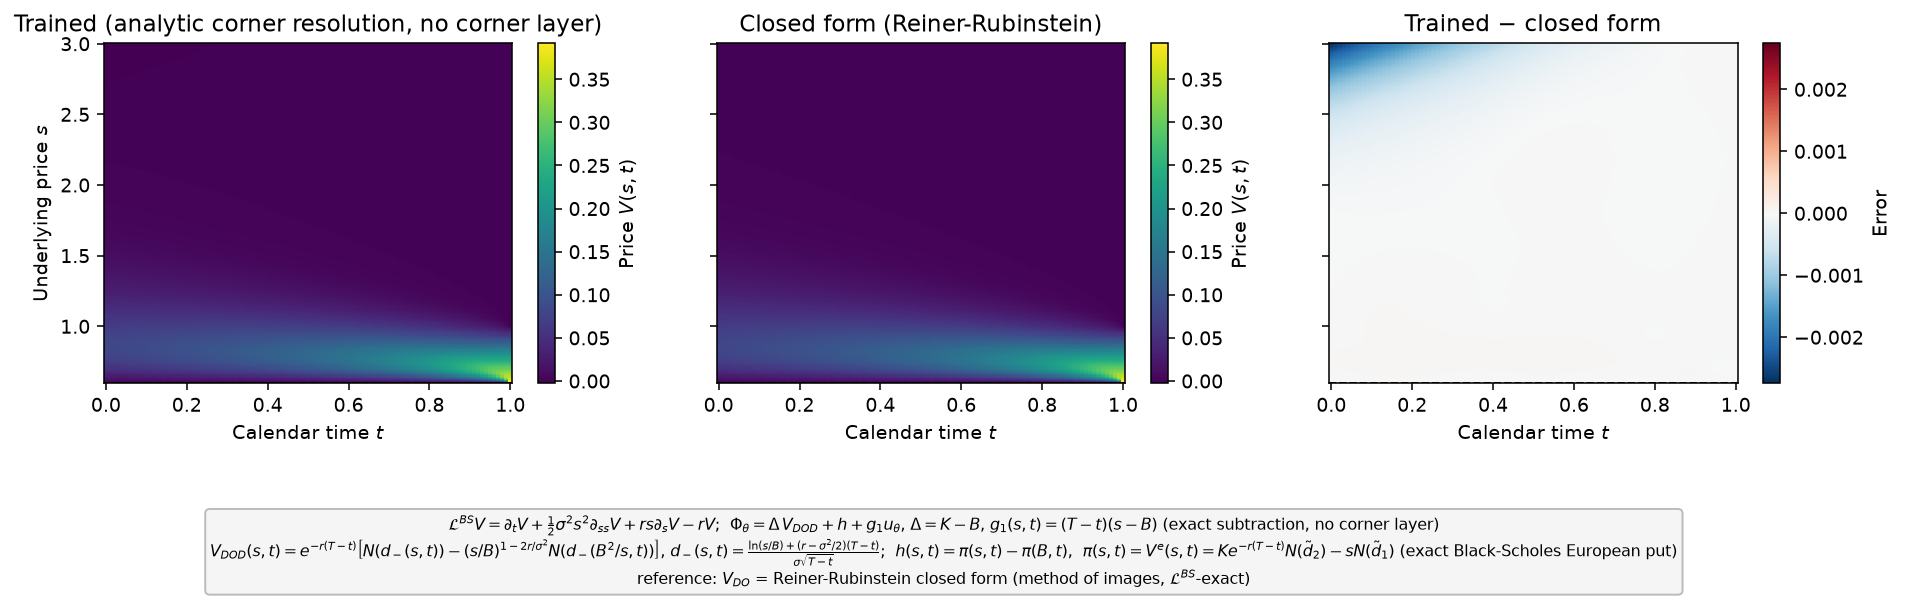
\includegraphics[width=\linewidth]{figures/subtraction_blackscholes_seed0_price_surface_eps0.png}
\caption{Surface de prix : solution entraînée, forme fermée, différence. soustraction exacte ($\Delta V_{DOD}$), profil Black--Scholes $V^e$.}
\label{fig:subtraction_blackscholes-price_surface_eps0}
\end{figure}

\begin{figure}[H]
\centering
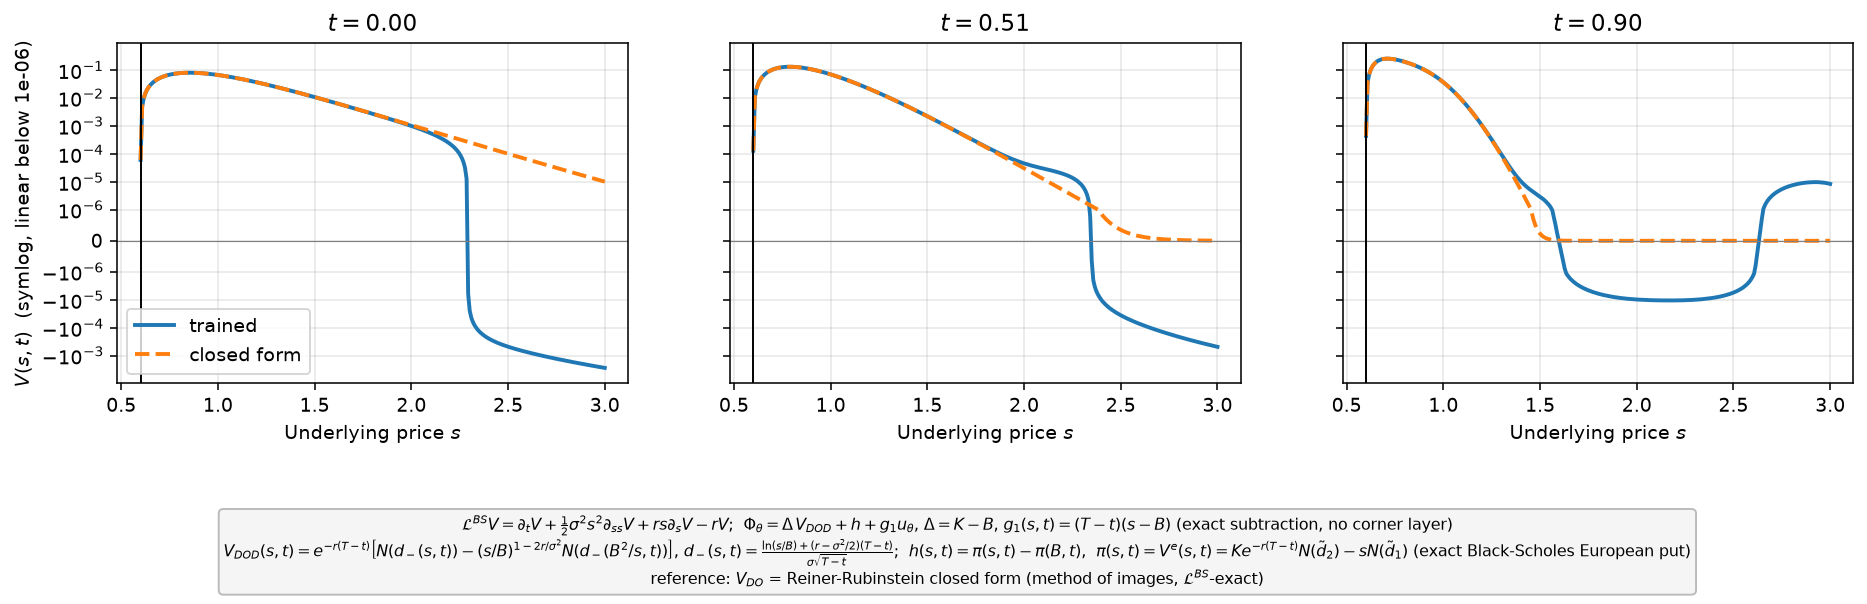
\includegraphics[width=\linewidth]{figures/subtraction_blackscholes_seed0_log_slice_eps0.png}
\caption{Coupes $V(s,t)$ à $t\in\{0,0.5,0.9\}$, échelle symlog (solution entraînée en trait plein, forme fermée en tirets ; trait vertical : $s=B$). soustraction exacte ($\Delta V_{DOD}$), profil Black--Scholes $V^e$.}
\label{fig:subtraction_blackscholes-log_slice_eps0}
\end{figure}

\begin{figure}[H]
\centering

\includegraphics[width=\linewidth]{figures/subtraction_blackscholes_seed0_subtraction_decomposition.png}
\caption{Décomposition de l'estimateur : partie singulière en forme fermée, extension régulière $h$, réseau $g_1u_\theta$, total, contre $V_{DO}$. soustraction exacte ($\Delta V_{DOD}$), profil Black--Scholes $V^e$.}
\label{fig:subtraction_blackscholes-subtraction_decomposition}
\end{figure}

\subsection{Exact subtraction, split-semigroup profile}
soustraction exacte ($\Delta V_{DOD}$), profil split-semigroupe. Run : \path{20260920_210040_iters50000_eps0_seed0_subtraction_split_nuc0.3_closedform}.
\begin{figure}[H]
\centering

\includegraphics[width=\linewidth]{figures/subtraction_split_seed0_price_surface_eps0.png}
\caption{Surface de prix : solution entraînée, forme fermée, différence. soustraction exacte ($\Delta V_{DOD}$), profil split-semigroupe.}
\label{fig:subtraction_split-price_surface_eps0}
\end{figure}

\begin{figure}[H]
\centering

\includegraphics[width=\linewidth]{figures/subtraction_split_seed0_log_slice_eps0.png}
\caption{Coupes $V(s,t)$ à $t\in\{0,0.5,0.9\}$, échelle symlog (solution entraînée en trait plein, forme fermée en tirets ; trait vertical : $s=B$). soustraction exacte ($\Delta V_{DOD}$), profil split-semigroupe.}
\label{fig:subtraction_split-log_slice_eps0}
\end{figure}

\begin{figure}[H]
\centering

\includegraphics[width=\linewidth]{figures/subtraction_split_seed0_subtraction_decomposition.png}
\caption{Décomposition de l'estimateur : partie singulière en forme fermée, extension régulière $h$, réseau $g_1u_\theta$, total, contre $V_{DO}$. soustraction exacte ($\Delta V_{DOD}$), profil split-semigroupe.}
\label{fig:subtraction_split-subtraction_decomposition}
\end{figure}

\subsection{Corner enrichment, raw payoff profile}
enrichissement du coin ($\chi\Delta\,\mathrm{erf}(\xi)$), profil payoff brut (contrôle négatif). Run : \path{20260921_003020_iters50000_eps0_seed0_enrichment_raw_d00.1_d10.3}.
\begin{figure}[H]
\centering

\includegraphics[width=\linewidth]{figures/enrichment_raw_seed0_price_surface_eps0.png}
\caption{Surface de prix : solution entraînée, forme fermée, différence. enrichissement du coin ($\chi\Delta\,\mathrm{erf}(\xi)$), profil payoff brut (contrôle négatif).}
\label{fig:enrichment_raw-price_surface_eps0}
\end{figure}

\begin{figure}[H]
\centering
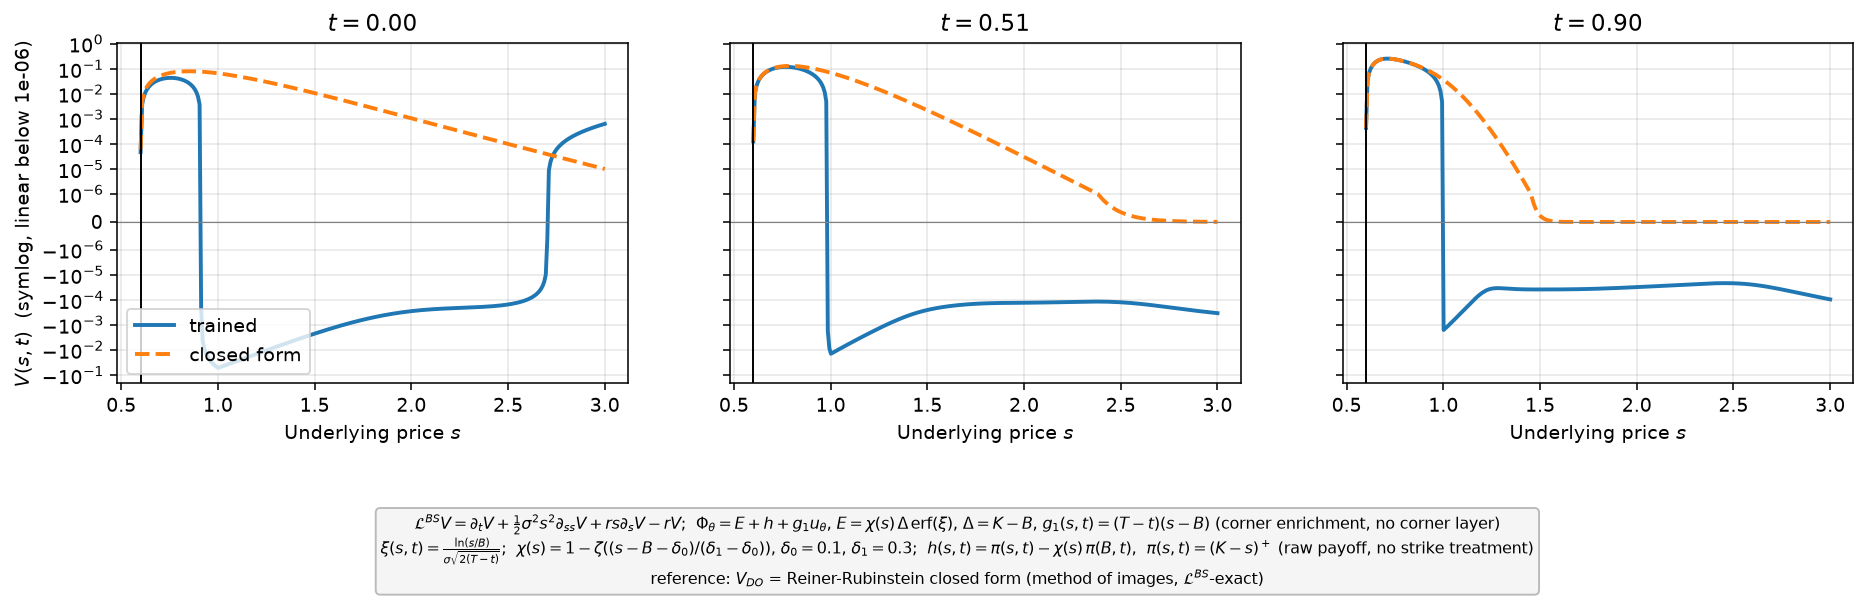
\includegraphics[width=\linewidth]{figures/enrichment_raw_seed0_log_slice_eps0.png}
\caption{Coupes $V(s,t)$ à $t\in\{0,0.5,0.9\}$, échelle symlog (solution entraînée en trait plein, forme fermée en tirets ; trait vertical : $s=B$). enrichissement du coin ($\chi\Delta\,\mathrm{erf}(\xi)$), profil payoff brut (contrôle négatif).}
\label{fig:enrichment_raw-log_slice_eps0}
\end{figure}

\begin{figure}[H]
\centering

\includegraphics[width=\linewidth]{figures/enrichment_raw_seed0_subtraction_decomposition.png}
\caption{Décomposition de l'estimateur : partie singulière en forme fermée, extension régulière $h$, réseau $g_1u_\theta$, total, contre $V_{DO}$. enrichissement du coin ($\chi\Delta\,\mathrm{erf}(\xi)$), profil payoff brut (contrôle négatif).}
\label{fig:enrichment_raw-subtraction_decomposition}
\end{figure}

\subsection{Corner enrichment, Black-Scholes profile}
enrichissement du coin ($\chi\Delta\,\mathrm{erf}(\xi)$), profil Black--Scholes $V^e$. Run : \path{20260921_003313_iters50000_eps0_seed0_enrichment_blackscholes_d00.1_d10.3}.
\begin{figure}[H]
\centering
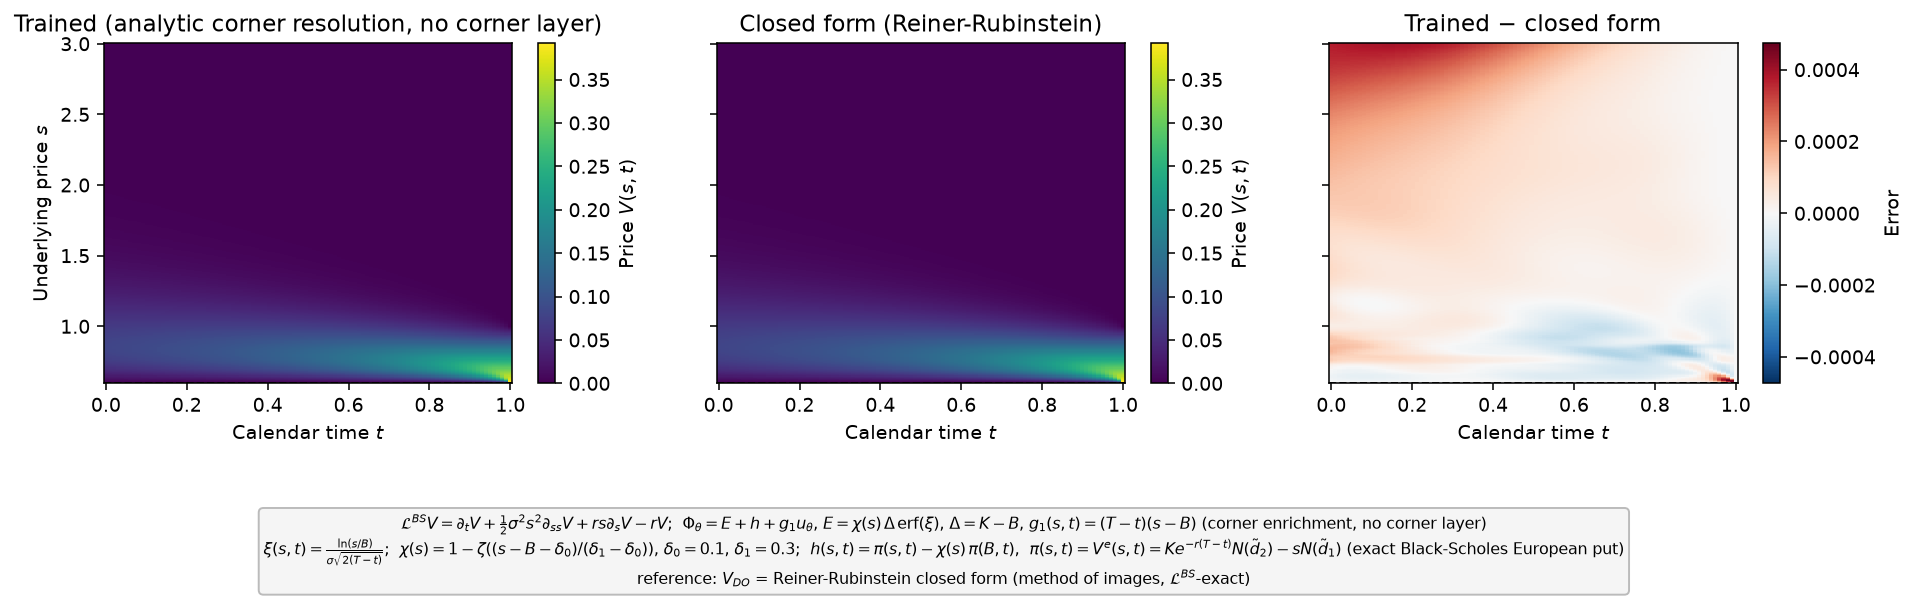
\includegraphics[width=\linewidth]{figures/enrichment_blackscholes_seed0_price_surface_eps0.png}
\caption{Surface de prix : solution entraînée, forme fermée, différence. enrichissement du coin ($\chi\Delta\,\mathrm{erf}(\xi)$), profil Black--Scholes $V^e$.}
\label{fig:enrichment_blackscholes-price_surface_eps0}
\end{figure}

\begin{figure}[H]
\centering
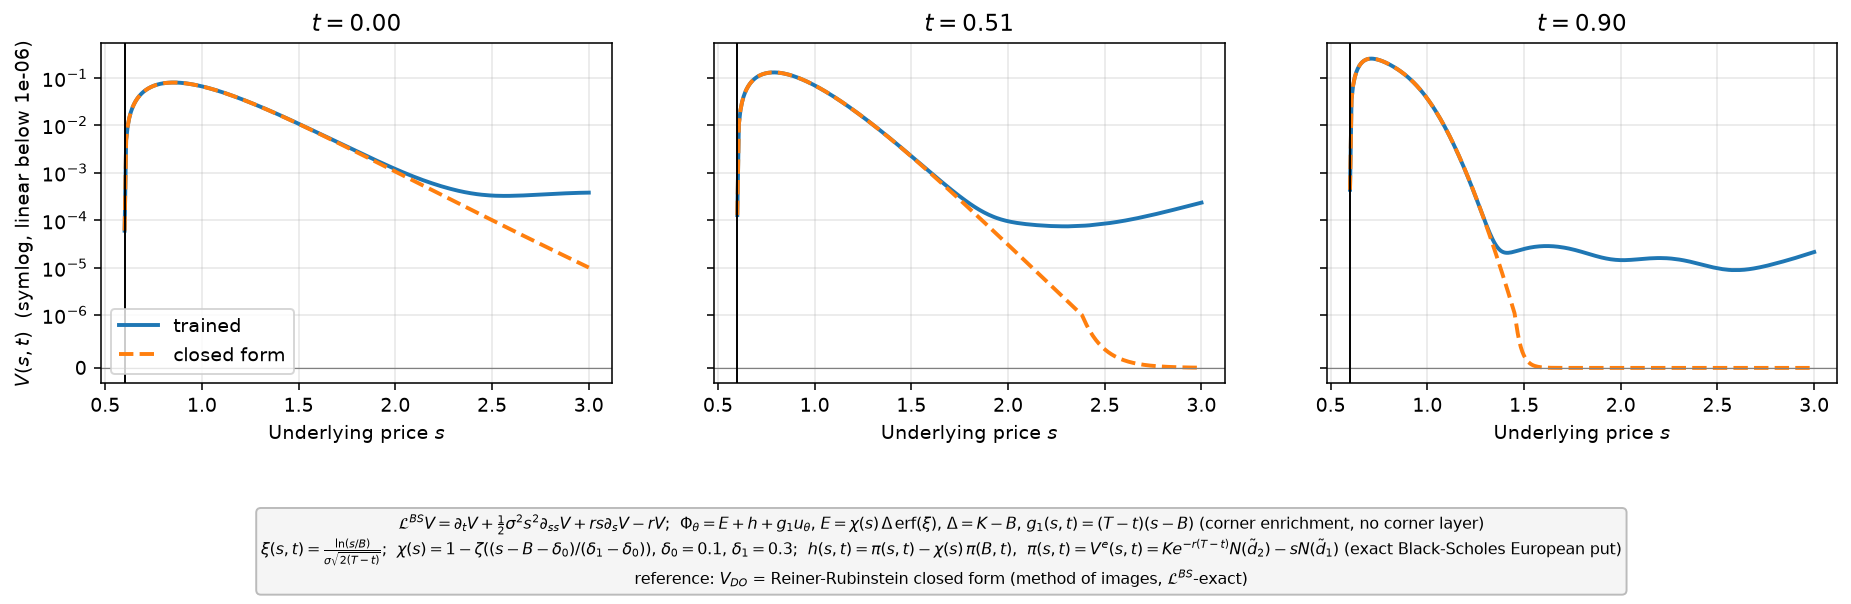
\includegraphics[width=\linewidth]{figures/enrichment_blackscholes_seed0_log_slice_eps0.png}
\caption{Coupes $V(s,t)$ à $t\in\{0,0.5,0.9\}$, échelle symlog (solution entraînée en trait plein, forme fermée en tirets ; trait vertical : $s=B$). enrichissement du coin ($\chi\Delta\,\mathrm{erf}(\xi)$), profil Black--Scholes $V^e$.}
\label{fig:enrichment_blackscholes-log_slice_eps0}
\end{figure}

\begin{figure}[H]
\centering

\includegraphics[width=\linewidth]{figures/enrichment_blackscholes_seed0_subtraction_decomposition.png}
\caption{Décomposition de l'estimateur : partie singulière en forme fermée, extension régulière $h$, réseau $g_1u_\theta$, total, contre $V_{DO}$. enrichissement du coin ($\chi\Delta\,\mathrm{erf}(\xi)$), profil Black--Scholes $V^e$.}
\label{fig:enrichment_blackscholes-subtraction_decomposition}
\end{figure}

\subsection{Corner enrichment, split-semigroup profile}
enrichissement du coin ($\chi\Delta\,\mathrm{erf}(\xi)$), profil split-semigroupe. Run : \path{20260921_011735_iters50000_eps0_seed0_enrichment_split_d00.1_d10.3_nuc0.3_closedform}.
\begin{figure}[H]
\centering

\includegraphics[width=\linewidth]{figures/enrichment_split_seed0_price_surface_eps0.png}
\caption{Surface de prix : solution entraînée, forme fermée, différence. enrichissement du coin ($\chi\Delta\,\mathrm{erf}(\xi)$), profil split-semigroupe.}
\label{fig:enrichment_split-price_surface_eps0}
\end{figure}

\begin{figure}[H]
\centering
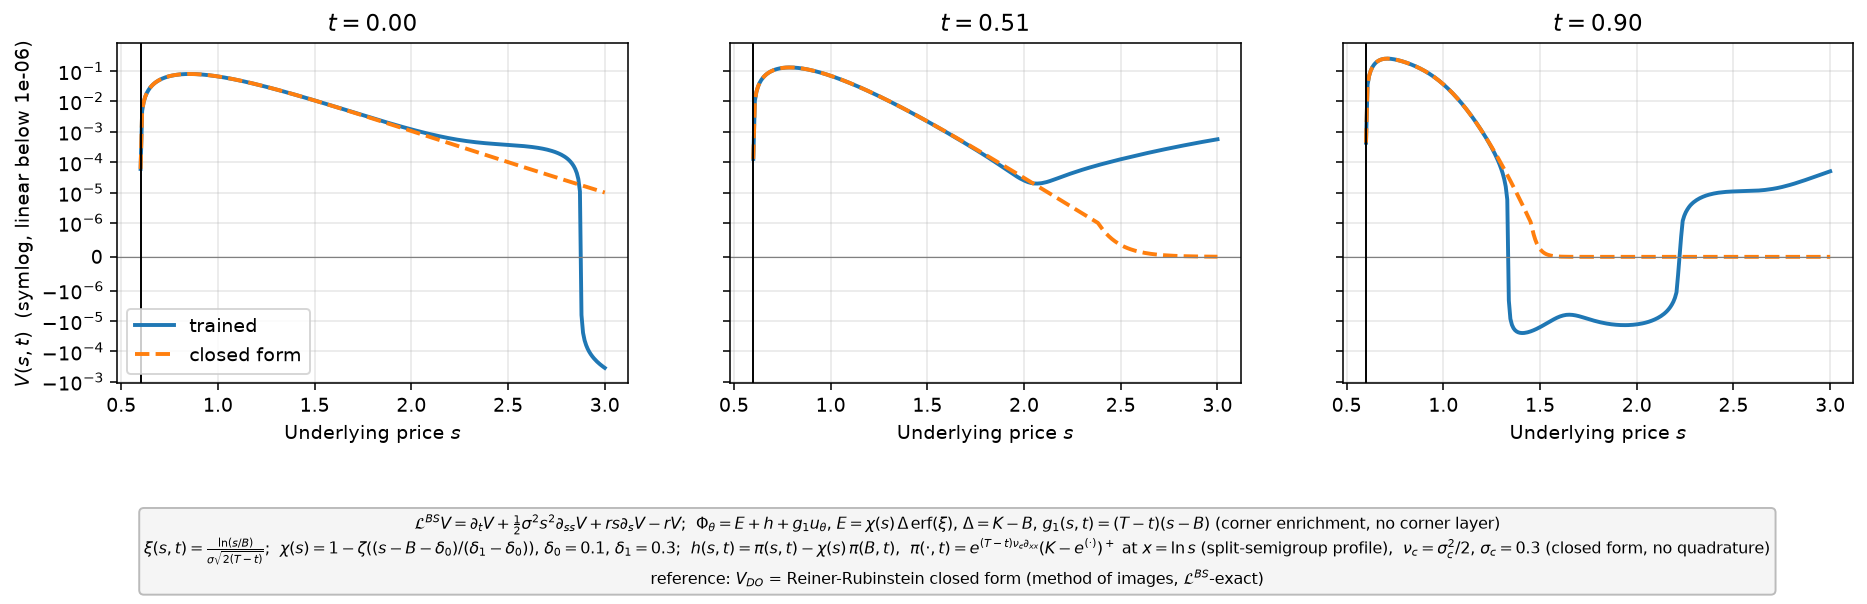
\includegraphics[width=\linewidth]{figures/enrichment_split_seed0_log_slice_eps0.png}
\caption{Coupes $V(s,t)$ à $t\in\{0,0.5,0.9\}$, échelle symlog (solution entraînée en trait plein, forme fermée en tirets ; trait vertical : $s=B$). enrichissement du coin ($\chi\Delta\,\mathrm{erf}(\xi)$), profil split-semigroupe.}
\label{fig:enrichment_split-log_slice_eps0}
\end{figure}

\begin{figure}[H]
\centering
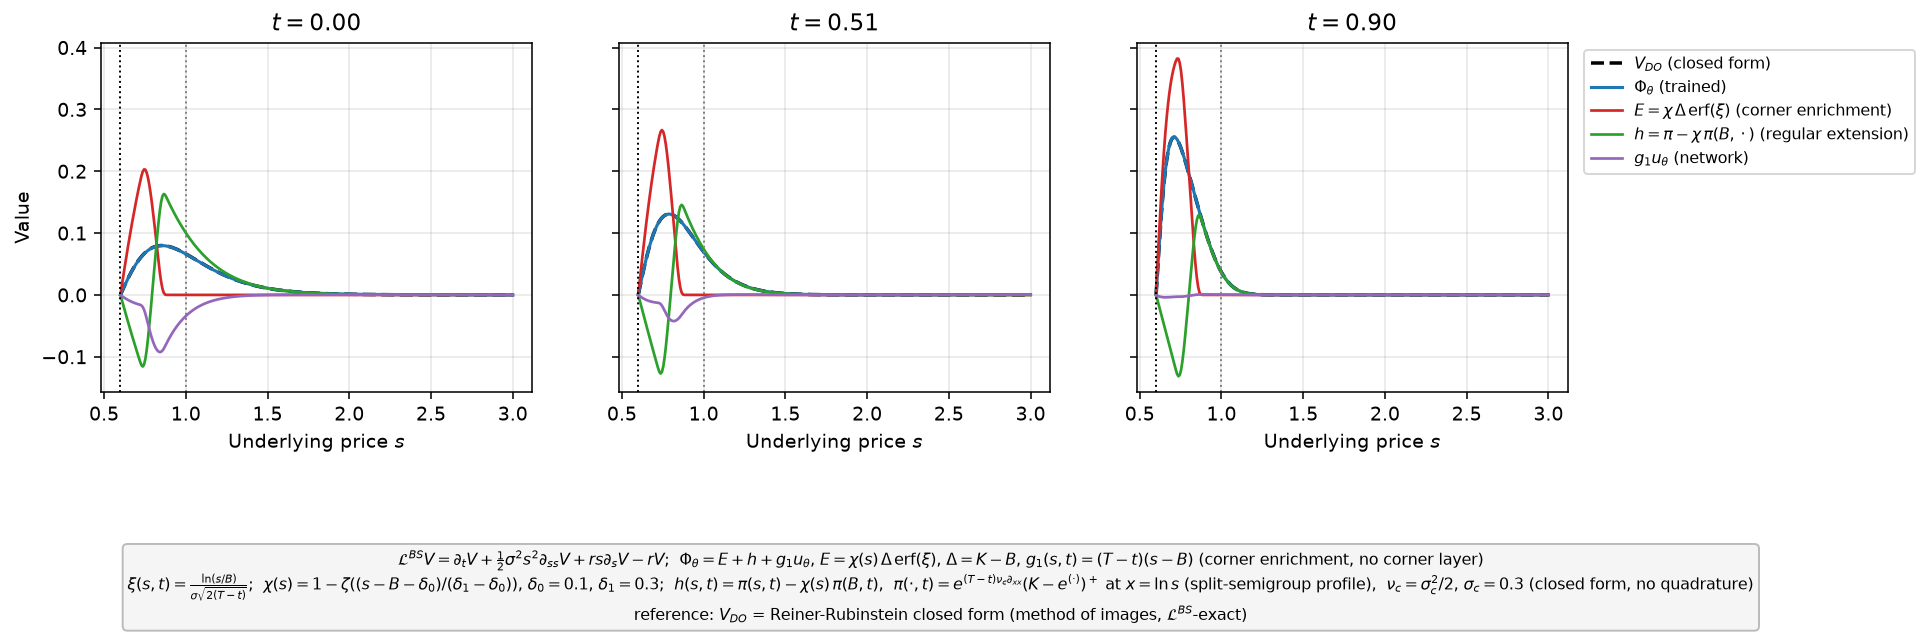
\includegraphics[width=\linewidth]{figures/enrichment_split_seed0_subtraction_decomposition.png}
\caption{Décomposition de l'estimateur : partie singulière en forme fermée, extension régulière $h$, réseau $g_1u_\theta$, total, contre $V_{DO}$. enrichissement du coin ($\chi\Delta\,\mathrm{erf}(\xi)$), profil split-semigroupe.}
\label{fig:enrichment_split-subtraction_decomposition}
\end{figure}

\end{document}
